\documentclass[a4paper,10pt]{book} %type de document et paramètres


\usepackage{lmodern} %police de caractère
\usepackage[english,french]{babel} %package de langues
\usepackage[utf8]{inputenc} %package fondamental
\usepackage[T1]{fontenc} %package fondamental

\usepackage[top=3cm, bottom=3cm, left=4cm, right=2cm]{geometry} %permet de paramétrer les marges par défaut
\usepackage{changepage} %permet de modifier localement une mise en page (marges,...) : utilisé pour la page de garde
%\usepackage{multicol} %permet de mettre plusieurs colonnes (\begin{multicols}{2} \end{multicols} jusqu'à 10 colonnes)
\usepackage[pdftex, pdfauthor={Pierre Gimalac}, pdftitle={Modèle}, pdfsubject={LaTeX}, pdfkeywords={LaTeX}, colorlinks=true, linkcolor=black]{hyperref} %permet de se déplacer dans le pdf depuis le sommaire en cliquant sur les titres, ainsi que de parametrer les meta données du PDF
%\usepackage{url} %permet de mettre des URL actifs \url{}
%\let\urlorig\url
%\renewcommand{\url}[1]{\begin{otherlanguage}{english}\urlorig{#1}\end{otherlanguage}}

\usepackage{mathtools} %maths (à developper, utile par exemple pour enlever les espaces dus aux boites $\sum_{\mathclap{1\le i\le j\le n}} X_{ij}$)
\usepackage{amssymb} %maths
\usepackage{amsthm} %maths
\usepackage{amsmath} %maths
\usepackage{mathrsfs} %maths (par exemple les lettres caligraphiées)
\usepackage{stmaryrd} %maths (par exemple les ensembles d'entiers \rrbracket \llbracket)
\usepackage{calrsfs} %maths (par exemple les notations des ensembles)
\usepackage{yhmath} % permet de noter les arcs de cercle avec \wideparen{AOB}
\usepackage{xlop} %permet d'afficher des opérations mathématiques
%\usepackage[squaren,Gray]{SIunits} %permet de noter des unités proprement
%\usepackage{esdiff} %permet d'écrire la dérivée avec la notation de Leibniz \diff{v}{t}

\usepackage{graphicx} %permet d'insérer des images proprement (ajoute des parametres)
\usepackage{wrapfig} %permet de mettre des images à coté d'un texte
%\usepackage{pdfpages} %permet d'insérer un pdf \includepdf[pages={1-2}]{truc.pdf}
\usepackage{enumitem} %permet de changer le label d'une liste \begin{itemize}[label=$\cdot$]
%\usepackage{ulem} %permet de souligner/barrer du texte
%\usepackage{soul} %permet de souligner/barrer du texte
%\usepackage{cancel} %permet de barrer du texte /cancel{text}


\usepackage{tikz} %package trooop bien permet de dessiner tout et n'importe quoi ! \begin{tikzpicture}
%\usepackage{circuitikz} %permet de dessiner des circuits logiques (entre autre) avec la syntaxe de tikz (\begin{circuitikz}) par exemple \node[american not port] pour le 'non'
%\usepackage{listings} %permet d'inserer du code dans le fichier (\lstset{language=Java} \begin{lstlisting} \end{lstlisting} )


\newcommand{\R}{\mathbb{R}}
\newcommand{\Rpe}{\mathbb{R}_{+}^{*}}
\newcommand{\N}{\mathbb{N}}
\newcommand{\Z}{\mathbb{Z}}
\newcommand{\C}{\mathbb{C}}
\newcommand{\Q}{\mathbb{Q}}
\newcommand{\K}{\mathbb{K}}
\newcommand{\Rb}{\overline{\mathbb{R}}}
%\newcommand\fra[2]{\genfrac{}{}{0pt}{1}{#1}{#2}}
\newcommand{\equi}[1]{\renewcommand{\arraystretch}{0.3}~\begin{matrix}\sim\\#1\end{matrix}~\renewcommand{\arraystretch}{1}}
\newcommand{\dl}{développement limité }
\newcommand{\evs}{espaces vectoriels }
\newcommand{\ev}{espace vectoriel }
\newcommand{\sevs}{sous-espaces vectoriels }
\newcommand{\sev}{sous-espace vectoriel }
\newcommand{\abs}[1]{\left|#1\right|}
\newcommand{\tq}{~|~}
\newcommand{\dls}{développements limités }
\newcommand{\displayAmath}{\displaystyle}
\newcommand{\lime}[4]{#1\underset{\mathclap{#2 \rightarrow #3}}{\longrightarrow} #4}
\newcommand{\supp}{\mathrm{supp}~} % support
\newcommand{\Ima}{\mathrm{Im}~} % image
\newcommand{\Inv}{\mathrm{Inv}~} % nombre d'inversion d'une permutation
\newcommand{\ord}{\mathrm{ord}~} % ordre
\newcommand{\com}{\mathrm{com}~} % comatrice

\begin{document}

\begin{titlepage}
\newgeometry{margin=2.7cm}
\thispagestyle{empty}
\begin{center}
\vspace*{6.7cm}
\Huge \textsc{Algèbre et Analyse\\ Approfondies I}\\
\vspace{1.5cm}
\Large Pierre Gimalac\\
\vspace{0.2cm}
\normalsize\textit{Avec l'aide précieuse de Xavier Durand}\\
\small \textit{Et la participation exceptionnelle du cours de Maxime Flin page \pageref{maxime}}\\
\vspace{0.5cm}
\large \textit{Licences de Mathématiques et d'Informatique}
\vfill
\end{center}
\large \textit{Septembre - Décembre 2017}
\hfill
\large Cours de Jaouad Sahbani
\restoregeometry
\end{titlepage}

\renewcommand{\contentsname}{Sommaire}
\thispagestyle{empty}
\tableofcontents
\thispagestyle{empty}

\part{Analyse}


\chapter{Comparaison locale des fonctions}
\section{Introduction}
\subsection{Rappels}
\subsubsection{Ensembles}
On appelle $\R$ le corps des nombres réels et $\Rb=\R \cup \{-\infty ; + \infty \}$ muni des règles et conventions de calcul usuelles.

\subsubsection{Voisinage}
Soit a $\in \Rb$ :
\begin{enumerate}
\item Si $a \in \R$, un voisinage de $a$ est une partie de $\R$ contenant un intervalle\\ de la forme $]a-\eta ; a+\eta[$ avec $\eta>0$.
\item Si $a =+\infty$, un voisinage de $a$ est une partie de $\R$ contenant un intervalle\\ de la forme $]A;+\infty[$ avec $A\in \R$.
\item Si $a = -\infty$, un voisinage de $a$ est une partie de $\R$ contenant un intervalle\\ de la forme $]-\infty ; A[$ avec $A\in \R$.
\end{enumerate}

\bigskip

Les voisinages de $a$ seront notés par $V$.

\subsubsection{Propriété}
On dira qu'une fonction $f$ vérifie une propriété $P(x)$ au voisinage de $a$ s'il existe un voisinage $V$ de $a$ sur lequel $f(x)$ vérifie la propriété $P(x)$.

\subsection{Position du problème}
Soient $a\in\Rb$ et deux fonctions $f,g$ définies au voisinage de a sauf peut-être au point $a$.\\
On a $\lim\limits_{x\rightarrow a}f(x)=0$ et $\lim\limits_{x\rightarrow a}g(x)=0$. On veut comparer $f(x)$ et $g(x)$ quand $x$ tend vers $a$.

\subsubsection{Exemples}
\begin{enumerate}
\item Si $f(x)=x^2$ et $g(x)=\sqrt{x}$, on a bien $\lim\limits_{x\rightarrow a}x^2=0$ et $\lim\limits_{x\rightarrow a}\sqrt{x}=0$.

Une façon d'aborder le problème est celle d'étudier, $\forall x\neq 0$, $\frac{f(x)}{g(x)}=x\sqrt{x}$ : $\lim\limits_{x\rightarrow 0}x\sqrt{x}=0$.

On a alors que $f(x)=x^2$ est négligeable (voir \ref{negligeable} page \pageref{negligeable}) devant $g(x)=\sqrt{x}$.\\

\item
Si $f(x)=\sin(x)$ et $g(x)=x$, $\frac{f(x)}{g(x)}=\frac{\sin(x)}{x}$ et $\lim\limits_{x\rightarrow 0} \frac{\sin(x)}{x}=1$ donc $f(x)=\sin(x)$ et $g(x)=x$ sont équivalentes (voir \ref{equivalente} page \pageref{equivalente}) en $0$.
\end{enumerate}

\newpage

\section{Relation de domination}
Soient $a \in \Rb$ et $f$ et $g$ deux fonctions définies au voisinage de $a$, sauf peut-être en $a$.

\subsection{Définition}
On dit que $f$ est dominée par $g$ au voisinage de $a$ s'il existe un voisinage $V$ de $a$ et une fonction $M$ définie sur $V\backslash\{a\}$ tels que $f(x)=M(x)g(x)$ avec $M$ bornée ($\exists c>0$ | $\forall x\in V\backslash \{a\}, |M(x)|\leq c$).\\

En particulier, si $g$ ne s'annule pas sur $V\backslash \{a\}$ alors $f$ dominée par $g$ signifie que $\frac{f(x)}{g(x)}$ est bornée au voisinage de $a$.

\subsection{Notation}
Dans ce cas, on notera $f=O_a(g)$ que l'on lit "$f$ est égale à grand o de $g$ au voisinage de $a$".

\subsection{Exemples}
\begin{itemize}[label=$\bullet$]
\item Si $g=1$, alors $f=O_a(g)=O_a(1)$ signifie que $f$ est bornée sur un voisinage de $a$.\\

\item Soit $f(x)=\sin(\frac{1}{x})$, $f=O_a(1)$ car $|\sin(\frac{1}{x})|\leq 1$, $\forall x\neq 0$.\\

\item Soient $f(x)=x^2 \sin(\frac{1}{x})$ et $g(x)=x^2$, $f=O_0(g)$ et $f=O_{+\infty}(g)$.\\

\item Soient $f(x)=\frac{1}{x}+x-2=\frac{1}{x}(x-1)^2$ et $g(x)=(x-1)^2$,\\
$M(x)=\frac{1}{x}$ est bornée au voisinage de 1 donc $f=O_1(g)$.

\end{itemize}

\subsection{Propriétés}
\begin{enumerate}
\item Si $f=O_a(g)$ et $g=O_a(h)$ alors $f=O_a(h)$.\\
\item Si $f_1=O_a(g)$ et $f_2=O_a(g)$ alors $(f_1+f_2)=O_a(g)$.\\
\item Si $f_1=O_a(g_1)$ et $f_2=O_a(g_2)$ alors $(f_1f_2)=O_a(g_1g_2)$.
\end{enumerate}

\subsubsection{Démonstration}
\begin{enumerate}
\item $f=O_a(g)$ et $g=O_a(h)$ $\Leftrightarrow \exists M_1,M_2$ bornées telles que $f(x)=M_1(x)g(x)=M_2(x)M_1(x)h(x)$.\\
Or $M_1M_2$ est bornée en tant que produit de fonctions bornées donc $f=O_a(h)$.\\
\item $f_1=O_a(g)$ et $f_2=O_a(g)$ $\Leftrightarrow \exists M_1,M_2$ bornées telles que $f_i(x)=M_i(x)g(x)$ $\forall i\in \{1;2\}$.\\
Alors $f_1(x)+f_2(x)=g(x)(M_1(x)+M_2(x))$ et $M_1+M_2$ est bornée donc $(f_1+f_2)=O_a(g)$.\\
\item $f_1=O_a(g_1)$ et $f_2=O_a(g_2)$ $\Leftrightarrow \exists M_1,M_2$ bornées telles que $f_i(x)=M_i(x)g_1(x)$ $\forall i\in \{1;2\}$.\\
Alors $f_1(x)f_2(x)=M_1(x)M_2(x)g_1(x)g_2(x)$ et $M_1M_2$ est bornée donc $(f_1f_2)=O_a(g_1g_2)$.
\end{enumerate}

\newpage

\section{Relation de prépondérance}\label{negligeable}
Soient $a \in \Rb$ et deux fonctions $f$ et $g$ définies sur un voisinage de $a$ (sauf peut-être au point $a$).

\subsection{Définition}
On dit que $f$ est négligeable devant $g$ au voisinage du point $a$ s'il existe un voisinage $V$ de $a$ et une fonction $\epsilon$ définie dans ce voisinage tels que $f(x)=\epsilon(x)g(x)$ $\forall x\in V\backslash \{a\}$ et $\lim\limits_{x\rightarrow a}\epsilon(x)=0$.\\

En particulier, si $g$ ne s'annule pas sur le voisinage de $a$ alors $f$ est négligeable devant $g$ au voisinage de $a$ signifie que $\lim\limits_{x\rightarrow a} \frac{f(x)}{g(x)}=0$

\subsection{Notation}
Dans ce cas on notera $f=o_a(g)$. On lira "$f$ égale à petit $o$ de $g$ au voisinage de $a$".

\subsection{Exemples}
\begin{itemize}[label=$\bullet$]
\item Supposons que $g=1$, alors $f=o_a(g)=o_a(1) \Leftrightarrow \lim\limits_{x\rightarrow a}f(x)=0$.
\item Si $f(x)=x^2\sin(\frac{1}{x})$ et $g(x)=x^2$, on a $f=o_{+\infty}(g)$.
\item Si $f(x)=\ln(x)$ et $g(x)=x$, $\lim\limits_{x\rightarrow +\infty} \frac{f(x)}{g(x)}=0$ et donc $\ln(x)=o_{+\infty}(x)$.
\end{itemize}

\subsection{Propriétés}
\begin{enumerate}
\item Si $f=o_a(g)$ et $g=O_a(h)$ alors $f=o_a(h)$.
\item Si $f_1=o_a(g)$ et $f_2=o_a(g)$ alors $f_1+f_2=o_a(g)$.
\item Si $f_1=o_a(g_1)$ et $f_2=O_a(g_2)$ alors $f_1f_2=o_a(g_1g_2)$.
\end{enumerate}

\subsubsection{Démonstrations}
\begin{enumerate}
\item $\left\{\begin{array}{rcl} f&=& o_a(g) \\ g&=& O_a(h)\end{array} \right.
\Leftrightarrow \left\{\begin{array}{rcl} f(x)=\epsilon(x)g(x)&\text{ avec }&\lim\limits_{x\rightarrow a}\epsilon(x)=0 \\ g(x)=M(x)h(x)&\text{ avec }&|M(x)|\leq C\text{, }C>0\text{, }\forall x\in V\backslash\{a\}\end{array}\right.$

Ainsi $f(x)=\epsilon(x) g(x)=\epsilon(x)M(x)h(x)$, on pose $\epsilon_1(x)=\epsilon(x)M(x)$

or $0\leq |\epsilon_1(x)|=|\epsilon(x)|\cdot |M(x)| \leq C\cdot |\epsilon(x)|$ sur un voisinage de $a$ et enfin $\lim\limits_{x\rightarrow a}\epsilon_1(x)=0$.

\bigskip

\item $\left\{\begin{array}{rcl} f_1&=& o_a(g) \\ f_2&=& o_a(g)\end{array} \right.
\Leftrightarrow \left\{\begin{array}{rcl} f_1(x)=\epsilon_1(x)g(x)&\text{ avec }&\lim\limits_{x\rightarrow a}\epsilon_1(x)=0 \\ f_2(x)=\epsilon_2(x)g(x)&\text{ avec }&\lim\limits_{x\rightarrow a}\epsilon_2(x)=0\end{array}\right.$

Alors $f_1(x)+f_2(x)=\epsilon_1(x)g(x)+\epsilon_2(x)g(x)=(\epsilon_1(x)+\epsilon_2(x))g(x)$ et $\lim\limits_{x\rightarrow a}\epsilon_1(x)+\epsilon_2(x)=0$.

\bigskip

\item $\left\{\begin{array}{rcl} f_1&=& o_a(g_1) \\ f_2&=& O_a(g_2)\end{array} \right.
\Leftrightarrow \left\{\begin{array}{rcl} f_1(x)=\epsilon_1(x)g_1(x)&\text{ avec }&\lim\limits_{x\rightarrow a}\epsilon_1(x)=0 \\ f_2(x)=M(x)g_2(x)&\text{ avec }&|M(x)|\leq C\text{, }C>0\text{, }\forall x\in V\backslash\{a\}\end{array}\right.$

Ainsi $f_1(x)f_2(x)=\epsilon_1(x)M(x)g_1(x)g_2(x)$, on pose $\epsilon(x)=\epsilon_1(x)M(x)$

or $0\leq |\epsilon(x)|=|\epsilon_1(x)|\cdot |M(x)| \leq C\cdot |\epsilon_1(x)|$ sur un voisinage de $a$ et enfin $\lim\limits_{x\rightarrow a}\epsilon(x)=0$.
\end{enumerate}

\subsection{Exemples fondamentaux}
\begin{enumerate}
\item Les puissances en 0 : $\forall m,n\in \Rpe {}^2$, $n>m$, $\frac{x^n}{x^m}=x^{n-m}$ et $\lim\limits_{x\rightarrow 0} x^{n-m}=0$ donc $x^n=o_0(x^m)$.

\item Les puissances à l'infini : $\forall m,n\in \Rpe {}^2$, $n>m$, $\frac{x^m}{x^n}=x^{m-n}$ et $\lim\limits_{x\rightarrow +\infty} x^{m-n}=0$\\donc $x^m=o_{+\infty}(x^n)$.

\smallskip

\item $\forall \alpha>0$, $x^\alpha=o_{+\infty}(e^x)$ car $\lim\limits_{x\rightarrow+\infty}\frac{x^\alpha}{e^x}=0$.

\item $\forall \alpha, \beta\in \Rpe{}^2$, $(\ln(x))^\alpha=o_{+\infty}(x^\beta)$.
\end{enumerate}

\newpage

\section{Équivalence des fonctions}\label{equivalente}
Soient $a \in \Rb$ et $f$ et $g$ deux fonctions définies au voisinage de $a$ (sauf peut être au point $a$).

\subsection{Définition}
On dit que $f$ est équivalente à $g$ au voisinage de $a$ si $f-g=o_a(g)$.

\subsection{Notation}
Si $f$ est équivalente à $g$ au point $a$, on note $f\equi{a}g$.

\subsection{Observation}
Si sur un voisinage $V$ de $a$ on a $f(x)-g(x)=\epsilon(x)g(x)$ et $\lim\limits_{x\rightarrow a}\epsilon(x)=0$ alors $f(x)=(1+\epsilon(x))g(x)$.\\
Autrement dit $f\equi{a}g$ signifie qu'il existe au voisinage $V$ de $a$ une fonction $\epsilon(x)$ telle que\\
$\forall x\in V\backslash\{a\}$, $f(x)=(1+\epsilon(x))g(x)$ et $\lim\limits_{x\rightarrow a}\epsilon(x)=0$.\\

Si $g$ ne s'annule pas sur un voisinage de $a$ alors $f\equi{a}g \Leftrightarrow \lim\limits_{x\rightarrow a}\frac{f(x)}{g(x)}=1$.

\subsection{Exemples}
\begin{enumerate}
\item $\sin(x) \equi{0} x$ car $\lim\limits_{x\rightarrow 0} \frac{\sin(x)}{x}=1$.

\item $\sin(\frac{1}{x})\equi{+\infty}\frac{1}{x}$ car $\displaystyle\lim\limits_{x\rightarrow +\infty} \frac{\sin(\frac{1}{x})}{\frac{1}{x}}=\lim\limits_{x\rightarrow 0}\frac{\sin(x)}{x}=1$.
\end{enumerate}

\subsection{Propriétés}
\begin{enumerate}
\item Symétrie : si $f \equi{a} g$ alors $g \equi{a} f$.
\item Transitivité : si $f \equi{a} g$ et $g \equi{a} h$ alors $f \equi{a} h$.
\item Réflexivité : $f \equi{a} f$.
\end{enumerate}
\smallskip
Ainsi $\sim$ est une relation d'équivalence.

\subsubsection{Démonstrations}
\begin{enumerate}
\item Supposons que $f \equi{a} g$ alors $\exists h$ une fonction définie sur un voisinage de $a$ telle que\\
$f(x)=h(x)g(x)$ et $\lim\limits_{x\rightarrow a}h(x)=1$.\\

Par définition de la limite, pour $\epsilon=\frac{1}{2}$, $\exists \eta>0$ tel que $|x-a|<\eta \Rightarrow |h(x)-1|<\frac{1}{2}$.\\

Ainsi $a-\eta<x<a+\eta \Rightarrow \frac{1}{2}\leq h(x)\leq \frac{3}{2}$ et sur $]a-\eta ; a+\eta[$, $h$ ne s'annule pas.\\

D'où $\forall x\in ]a-\eta ; a+\eta[$, $g(x)=\frac{1}{h(x)}f(x)$ et $\lim\limits_{x\rightarrow a}\frac{1}{h(x)}=1$ donc $g \equi{a} f$.

\bigskip

\item Si l'on a $f \equi{a} g$ et $g \equi{a} h$ alors $\exists h_1,h_2$ telles que $f=h_1g$, $g=h_2h$ et $\lim\limits_{x\rightarrow a}h_1(x)=\lim\limits_{x\rightarrow a}h_2(x)=1$.

Ainsi $f(x)=h_1(x)g(x)=h_1(x)h_2(x)h(x)=h_3(x)h(x)$ avec $h_3=h_1h_2$ et $\lim\limits_{x\rightarrow a}h_3(x)=1$.

\bigskip

\item En prenant $\epsilon$ la fonction définie par $\epsilon(x)=1$, on a trivialement que $f(x)=\epsilon(x)f(x)$ et $\lim\limits_{x\rightarrow a}\epsilon(x)=1$ d'où enfin $f \equi{a} f$.
\end{enumerate}

\newpage

\subsection{Propositions}
\begin{enumerate}
\item Soit $l\in \R$, si $f \equi{a} g$ et si $\lim\limits_{x\rightarrow a}g(x)=l$ alors $\lim\limits_{x\rightarrow a}f(x)=l$.
\item Soient $l\in \R^*$ et $f$ telle que $\lim\limits_{x\rightarrow a}f(x)=l$, alors $f\equi{a}l$.
\end{enumerate}

\subsubsection{Démonstration}
\begin{enumerate}
\item Si $f \equi{a} g$ alors sur un voisinage de $a$, $\exists h$ telle que $f(x)=h(x)g(x)$ et $\lim\limits_{ x\rightarrow a}h(x)=1$.\\
Ainsi $\lim\limits_{x\rightarrow a}f(x)=1\cdot l=l$.
\item $\displaystyle\lim\limits_{x\rightarrow a}\frac{f(x)}{l}=\frac{l}{l}=1$ donc $f\equi{a}l$.
\end{enumerate}

\subsubsection{Exemples}
\begin{enumerate}
\item $\cos(x) \equi{0} 1$.
\item $e^x \equi{0} 1$.
\item $\cosh(x) \equi{0} 1$.
\end{enumerate}

\subsection{Théorème}
Soient $a \in \R$, $f$ une fonction définie sur un voisinage de $a$ et $f$ dérivable au point $a$.\\
Si $f'(a)\neq 0$ alors $f(x)-f(a) \equi{a} (x-a)f'(a)$.

\subsubsection{Démonstration}
$f$ est dérivable au point $a$ donc on a $\displaystyle\lim\limits_{x\rightarrow a} \frac{f(x)-f(a)}{x-a}-f'(a)=0$.\\
Soit $\displaystyle\epsilon(x)=\frac{f(x)-f(a)}{x-a}-f'(a)$ pour $x\neq a$, on a $\epsilon(x)(x-a)=f(x)-f(a)-(x-a)f'(a)$.\\

Enfin $\displaystyle f(x)-f(a)=(x-a)f'(a)\left[1+\frac{\epsilon(x)}{f'(a)}\right]=(x-a)f'(a)(1+\epsilon'(x))$ et $\lim\limits_{x\rightarrow a}\epsilon'(x)=0$.

\subsubsection{Exemples}
\begin{enumerate}
\item $\sin(x) \equi{0} x$.
\item $\ln(1+x) \equi{0} x$.
\item $\displaystyle\sqrt{1+x}-1 \equi{0} \frac{1}{2}x$.
\item $(1+x)^\alpha-1 \equi{0}\alpha x$.
\end{enumerate}\bigskip

\subsection*{Caractérisation de la relation de prépondérance}\label{prop1}
Soient $a \in \R$ et $f$ et $g$ deux fonctions définies au voisinage de $a$, alors $f=o_a(g)$ si et seulement si
$\forall \epsilon>0$, $\exists \eta>0 ~|~ 0<|x-a|<\eta\Rightarrow |f(x)|\leq \epsilon|g(x)|$.

\subsubsection*{Démonstration}
Si $f=o_a(g)$, on appelle $h$ la fonction définie au voisinage de $a$ par $h(x)=\frac{f(x)}{g(x)}$ si $g(x)\neq 0$ et $0$ sinon. $f(x)=h(x)g(x)=o_a(g)$ donc $\lim\limits_{x\rightarrow a}h(x)=0$ et $\forall \epsilon>0$, $\exists \eta>0 \tq 0<\abs{x-a}<\eta \Rightarrow \abs{h(x)}\leq\epsilon$.\\
Enfin, on a $\forall \epsilon>0$, $\exists \eta>0 ~|~ 0<|x-a|<\eta\Rightarrow |f(x)|\leq \epsilon|g(x)|$.\\

Si $\forall \epsilon>0$, $\exists \eta>0 ~|~ 0<|x-a|<\eta\Rightarrow |f(x)|\leq \epsilon|g(x)|$, on appelle $h$ la fonction définie au voisinage de $a$ par $h(x)=\frac{f(x)}{g(x)}$ si $g(x)\neq 0$ et $0$ sinon.

Si $g(x)=0$, $f(x)=0$ donc $f(x)=h(x)g(x)$ et $\forall \epsilon>0$, $\exists \eta>0 ~|~ 0<|x-a|<\eta\Rightarrow |h(x)|\leq \epsilon$, d'où en faisant tendre $\epsilon$ vers 0, $\lim\limits_{x\rightarrow a}h(x)=0$ et enfin $f=o_a(g)$.


\newpage

\section{Équivalence et opérations algébriques}
\subsection{Compatibilité avec le produit}
Si $f_1 \equi{a} g_1$ et $f_2 \equi{a} g_2$ alors $f_1f_2 \equi{a} g_1g_2$.

\subsubsection{Démonstration}
$f_1 \equi{a} g_1 \Rightarrow f_1=h_1(x)g_1(x)$ et $\lim\limits_{x\rightarrow a}h_1(x)=1$ ~;~
$f_2 \equi{a} g_2 \Rightarrow f_2=h_2(x)g_2(x)$ et $\lim\limits_{x\rightarrow a}h_2(x)=1$.

Ainsi $f_1f_2=(h_1h_2)(g_1g_2)$ avec $\lim\limits_{x\rightarrow a}h_1h_2=1$ par produit.

\subsubsection{Exemple}
$1-\cos(x)=2\sin^2(\frac{x}{2}) \equi{0} 2\cdot \frac{x}{2}\cdot \frac{x}{2}=\frac{x^2}{2}$.

\subsection{Compatibilité avec la division}
Si $f \equi{a} g$ et $g$ ne s'annule pas sur un voisinage de $a$ alors $\displaystyle\frac{1}{f} \equi{a} \frac{1}{g}$.

\subsubsection{Démonstration}
$f \equi{a} g \Rightarrow f(x)=h(x)g(x)$ où $\lim\limits_{x\rightarrow a}h(x)=1$. Comme $g$ ne s'annule pas sur un voisinage de $a$ on en déduit que $f$ ne s'annule pas sur un voisinage (pouvant être différent du premier) de $a$.\\

Enfin, $\frac{1}{f(x)}=\frac{1}{h(x)}\cdot \frac{1}{g(x)}$ avec $\lim\limits_{x\rightarrow a}\frac{1}{h(x)}=1$ par quotient.

\subsubsection{Exemple}
$\tan(x)=\frac{\sin(x)}{\cos(x)} \equi{0} \frac{x}{1}=x$.

\subsection{Compatibilité avec l'addition}
La relation d'équivalence au point $a$ n'est pas compatible avec l'addition.\\
Si $f_1 \equi{a} g_1$ et $f_2 \equi{a} g_2$, on n'a pas nécessairement que $f_1+f_2\equi{a} g_1+g_2$.\\

Cependant, si $f_1 \equi{a} g_1$, $f_2 \equi{a} g_2$ et $g_2=o_a(g_1)$ alors $f_1+f_2 \equi{a} g_1$.

\subsubsection{Démonstration}
On a $f_1=h_1g_1$ où $\lim\limits_{x\rightarrow a}h_1=1$ et $f_2=h_2g_2$ où $\lim\limits_{x\rightarrow a}h_2=1$.\\
De plus $g_2=\epsilon(x)g_1(x)$ et $\lim\limits_{x\rightarrow a}\epsilon(x)=0$. Ainsi $f_1+f_2=h_1g_1+h_2\epsilon g_2(x)=g(x)(h_1+\epsilon h_2)$.

\subsection{Théorème}
Si $f_1 \equi{a} g_1$, $f_2 \equi{a}g_2$ et $g_1,g_2$ ont le même signe sur un voisinage de $a$, alors $f_1+f_2 \equi{a} g_1+g_2$.

\subsubsection{Démonstration}
Par hypothèse, $f_1=(1+\epsilon_1(x))g_1(x)$, $f_2=(1+\epsilon_2(x))g_2(x)$ et $\lim\limits_{x\rightarrow a}\epsilon_1(x)=\lim\limits_{x\rightarrow a}\epsilon_2(x)=0$.\\

Soit $\epsilon=\left\{\begin{array}{clr}
0 &\text{ si }g_1(x)+g_2(x)=0 \\
\epsilon_1(x)\frac{g_1(x)}{g_1(x)+g_2(x)}+\epsilon_2(x)\frac{g_2(x)}{g_1(x)+g_2(x)} &\text{ sinon}
\end{array}\right.$\\

\smallskip

On a $|\frac{g_1(x)}{g_1(x)+g_2(x)}|\leq 1$ et $|\frac{g_2(x)}{g_1(x)+g_2(x)}|\leq 1$ donc $\lim\limits_{x\rightarrow a}\epsilon(x)=0$.\\

Enfin, $f_1+f_2=g_1+g_2+\epsilon_1g_1+\epsilon_2g_2=(1+\epsilon)(g_1+g_2)$ au voisinage de $a$.\\

\newpage

\section{Composition à droite (ou changement de variable)}
\subsection{Propriété}
Soient $a,b\in \Rb^2$, $u$ une fonction définie au voisinage de $a$ et $f,g$ deux fonctions définies au voisinage de $b=\lim\limits_{x\rightarrow a}u(x)$.

\begin{enumerate}
\item Si $f \equi{b} g$ alors $f \circ u \equi{a} g\circ u$.
\item Si $f=o_b(g)$ alors $f\circ u=o_a(g\circ u)$.
\item Si $f=O_b(g)$ alors $f\circ u = O_a(g\circ u)$.
\end{enumerate}

\subsubsection{Démonstration}
\begin{enumerate}
\item $\lim\limits_{x\rightarrow a}u(x)=b$ et $f \equi{b} g$
donc sur un voisinage $V_1$ de $b$, $f(x)=(1+\epsilon(x))f(x)$ et $\lim\limits_{x\rightarrow b}\epsilon(x)=0$.\\

$\lim\limits_{x\rightarrow a}u(x)=b$ donc il existe un voisinage $V_2$ de $a$ tel que $\forall x\in V_2$, $u(x)\in V_1$.\\

En effet, dans le cas où $a,b\in \R$ :

~~$\forall \alpha>0$, $\exists \beta>0$ tel que $|x-a|<\beta \Rightarrow |u(x)-b|<\alpha$

~~donc $a-\beta<x<a+\beta\Rightarrow b-\alpha<u(x)<b+\alpha$

~~et $x\in V_2=]a-\beta ; a+\beta[ ~\Rightarrow  u(x)\in V_1=]b-\alpha ;b+\alpha[$.\\

Ainsi $\forall x\in V_2$, $f(u(x))=(1+\epsilon(u(x)))g(u(x))$ et $\lim\limits_{x\rightarrow a}\epsilon(u(x))=0$.\\

\item $f=o_b(g)=\epsilon(x)g(x)$, avec $\lim\limits_{x\rightarrow b}\epsilon(x)=0$, alors $f\circ u(x)=\epsilon(u(x))(g\circ u)(x)$.\\
Or $\lim\limits_{x\rightarrow a}u(x)=b$ donc par composition $\lim\limits_{x\rightarrow b}\epsilon(u(x))=0$ et $f\circ u=o_a(g\circ u)$.\\

\item $f=O_b(g)$ donc $\exists M$ une fonction et $c>0 \tq \forall x\in V(b)\backslash \{b\}$, $f(x)=M(x)g(x)$ et $\abs{M(x)}\leq c$.\\
On sait que $\lim\limits_{x\rightarrow a}u(x)=b$ donc $\forall V(b)$, $\exists V(a) \tq \forall x\in V(a)\backslash\{a\}$, $u(x)\in V(b)\backslash\{b\}$,\\d'où $\exists V(a) \tq \forall x\in V(a)\backslash\{a\}$, $M(u(x))\in V(b)\backslash\{b\}$ et $\abs{M(u(x))}\leq c$, donc $f\circ u=O_a(g\circ u)$.
\end{enumerate}

\subsubsection{Exemples}
\begin{enumerate}
\item $\sin(\sqrt{|x|}) \equi{0} \sqrt{|x|}$ et $\sin(3x^3) \equi{0} 3x^3$.
\item $\ln(1+\frac{1}{x^2}) \equi{+\infty}\frac{1}{x^2}$.
\end{enumerate}

\subsection{Remarque}
Il n'y a pas de résultat similaire pour la composition à gauche :\\
$x^2+x \equi{+\infty} x^2$ et pourtant on n'a pas $e^{x+x^2} \equi{+\infty} e^{x^2}$.

\newpage

\section{Intégration}
Soient $a\in\R$ et $f$ une fonction dérivable au point $a$.

\subsection{Propriétés}
\begin{enumerate}
\item Si $f'=o_a((x-a)^n)$, alors $f(x)-f(a)=o_a((x-a)^{n+1})$
\item Si $f'\equi{a}(x-a)^n$ alors $f(x)-f(a)\equi{a}\frac{(x-a)^{n+1}}{n+1}$
\end{enumerate}

\subsubsection{Démonstration}
\begin{enumerate}
\item Supposons que $f'=o_a((x-a)^n)$.\\
D'après la proposition \ref{prop1} (page \pageref{prop1}), $\forall \epsilon>0$, $\exists \eta>0 \tq \forall x\in ]a-\eta ;a+\eta[$, $f'(x)\leq \epsilon|(x-a)^n|$.\\
Ainsi d'après le théorème fondamental de l'analyse, $\displaystyle\abs{f(x)-f(a)}=\abs{\int_{a}^{x}f'(t)dt}\leq \int_{a}^{x}\abs{f'(t)}dt$\\
\hspace*{12.15cm}$\displaystyle\leq \epsilon\int_{a}^{x}\abs{t-a}^ndt$

Si $x\geq a$ : $\displaystyle\epsilon\int_{a}^{x}\abs{t-a}^ndt=\epsilon \int_{a}^{x}(t-a)^ndt=\epsilon_1\frac{(x-a)^{n+1}}{n+1}\leq \epsilon_1\abs{x-a}^{n+1}$.

De même si $x\leq a$, d'où $f(x)-f(a)=o_a((x-a)^{n+1})$.\\

\item $f'\equi{a}(x-a)^n$ signifie que $f'(x)-(x-a)^n=o_a((x-a)^n)$ d'après la première propriété.\\

$\displaystyle f(x)-f(a)-\frac{(x-a)^{n+1}}{n+1}=o_a((x-a)^{n+1})$
qui est une autre façon d'écrire le résultat souhaité.
\end{enumerate}

\subsubsection{Exemples}
\begin{enumerate}
\item $\sin(x)\equi{0} x\Rightarrow 1-\cos(x)\equi{0}\frac{x^2}{2}$.
\item $e^x\equi{0}1 \Rightarrow e^x-1\equi{0}x$.
\item $1-\cos(x)\equi{0}\frac{x^2}{2}\Rightarrow x-\sin(x)\equi{0}\frac{x^3}{6}$.
\end{enumerate}

\section{Généralisation}
\subsection{Équivalent en un coté d'un point}
On peut parler des équivalents à droite d'un point $a\in \R$.\\

Par exemple, $f\equi{a_+}g\Leftrightarrow \left\{\begin{array}{rcl}f(x)=(1+\epsilon(x))g(x) & \forall x\in ]a; a+\eta[ \\ \lim\limits_{x\rightarrow a_+}\epsilon(x)=0\end{array}\right.$\\\\

$f=o_{a+}(g)\Leftrightarrow\exists \eta>0 \tq f(x)=\epsilon(x)g(x) ~\forall x\in ]a; a+\eta[$ et $\lim\limits_{x\rightarrow a+}\epsilon(x)=0$.

De même pour la gauche où il suffit de remplacer $a_+$ par $a_-$ et $]a;a+\eta[$ par $]a-\eta; a[$.

\subsubsection{Exemple}
Soient $f(x)=xe^{-\frac{1}{x}}$ et $g(x)=x$.\\
Comme $\lim\limits_{x\rightarrow0+}e^{-\frac{1}{x}}=0$, on conclue que $f=o_{a+}(g)$.\\
De même, $g(x)=xe^{-\frac{1}{x}}\cdot e^{\frac{1}{x}}=f(x)e^{\frac{1}{x}}$ et donc $g=o_{0-}(f)$ car $\lim\limits_{x\rightarrow 0^-}e^{\frac{1}{x}}=0$.

\newpage

\section{Rappels sur les formules de Taylor}
Dans tout cette section $I$ est un intervalle qui contient au moins deux points, $a\in I$ et\\$f$ est une fonction sur $I$ à valeurs réelles.

\subsection{Formule de Taylor avec reste intégral}
Si $f\in C^{n+1}$, $n\geq 0$, alors $\forall x\in I$,
$\displaystyle f(x)=\sum\limits_{k=0}^{n}\frac{(x-a)^k}{k!}f^{(k)}(a)+\int_{a}^{x}f^{(n+1)}(t)\frac{(x-t)^n}{n!}dt$.

\subsubsection{Démonstration}
On procède par récurrence sur $n$ :\\

Si $n=0$, $\displaystyle f(x)=f(a)+\int_{a}^{x}f'(t)dt$. Il s'agit du théorème fondamental de l'analyse.\\

Supposons que la formule est démontrée à l'ordre $n$ et que $f$ est $C^{n+2}$.\\
Alors d'après l'hypothèse de récurrence, $\displaystyle f(x)= \sum\limits_{k=0}^{n}\frac{(x-a)^k}{k!}f^{(k)}(a) +\int_{a}^{x}f^{(n+1)}(t)\frac{(x-t)^n}{n!}dt$.

$$\begin{array}{rcl}\displaystyle \int_{a}^{x}f^{(n+1)}(t)\frac{(x-t)^n}{n!}dt&=& \displaystyle-\left[f^{(n+1)}(t)\frac{(x-t)^{n+1}}{(n+1)!}\right]_a^x +\int_{a}^{x}f^{(n+2)}(t)\frac{(x-t)^{n+1}}{(n+1)!}dt\\\\
&=&\displaystyle f^{(n+1)}(t)\frac{(x-a)^{n+1}}{(n+1)!}+\int_{a}^{x}f^{(n+2)}(t)\frac{(x-t)^{n+1}}{(n+1)!}dt\end{array}$$

Ainsi $\displaystyle f(x)=\sum_{k=0}^{n+1}\frac{(x-a)^k}{k!}f^{(k)}(a)+\int_{a}^{x}f^{(n+2)}(t)\frac{(x-t)^{n+1}}{(n+1)!}dt$.

\subsection{Formule de Taylor-Lagrange}
Soit $f : [a;b] \rightarrow \R$ une fonction de classe $\mathcal{C}^{(n)}$ telle que $f^{(n+1)}$ existe sur $]a;b[$.\smallskip

Alors $\exists c\in ]a;b[$ tel que $\displaystyle f(b)=\sum\limits_{k=0}^n \left[\frac{(b-a)^k}{k!}f^{(k)}(a)\right]+\frac{(b-a)^{n+1}}{(n+1)!}f^{(n+1)}(c)$.

\subsubsection{Démonstration}
Par récurrence sur $n$, pour $n=0$, il s'agit de la formule des accroissements finis.\\

On prend un $n$ quelconque supérieur ou égal à 1 et on note\\$\displaystyle g(x)=f(b)-\sum\limits_{k=0}^n \left[\frac{(b-x)^k}{k!}f^{(k)}(x)\right]-A\frac{(b-x)^{n+1}}{(n+1)!}$ où $A$ est une constante telle que $g(a)=0$.\\

On a donc $\displaystyle f(b)=\sum\limits_{k=0}^n \left[\frac{(b-a)^k}{k!}f^{(k)}(a)\right]+A\frac{(b-a)^{n+1}}{(n+1)!}$.\\\\
$g(b)=0$ donc on peut appliquer le théorème de Rolle qui donne l'existence de $c \in ]a;b[\tq g'(c)=0$.\\\\
Or $\displaystyle g'(x)=\sum\limits_{k=1}^n \left[\frac{(b-x)^{k-1}}{(k-1)!}f^{(k)}(x)\right]-\sum\limits_{k=0}^n \left[\frac{(b-x)^k}{k!}f^{(k+1)}(x)\right]+A\frac{(b-x)^{n}}{n!}=\frac{(b-x)^{n}}{n!}\left[A-f^{(n+1)}(x)\right]$.\\\\

D'où $g'(c)=0$ implique $A=f^{(n+1)}(c)$ et $\displaystyle f(b)=\sum\limits_{k=0}^n \left[\frac{(b-a)^{k}}{k!}f^{(k)}(a)\right]+f^{(n+1)}(c)\frac{(b-a)^{n+1}}{(n+1)!}$.

\newpage

\subsection{Formule de Taylor-Young}
Soit $n\geq 1$, si $f$ est $n$ fois dérivable en $a$, alors $\displaystyle f(x)=\sum\limits_{k=0}^n\frac{f^{(k)}(a)}{k!}(x-a)^k+o_a((x-a)^n)$.

\subsubsection{Démonstration}
On procède par récurrence sur $n$ :\\\\\\
Pour $n=1$, la formule devient $f(x)=f(a)+(x-a)f'(a)+o_a(x-a)$.\\\\

Supposons par récurrence que la formule est démontrée à l'ordre $n\in\N^*$.\\

Supposons que $f$ est $n+1$ fois dérivable au point $a$, donc $f'$ est $n$ fois dérivable au point $a$ et on peut lui appliquer l'hypothèse de récurrence :
$\displaystyle f'(x)=\sum\limits_{k=0}^n\frac{f^{(k+1)}(a)}{k!}(x-a)^k+o_a((x-a)^n)$.

La règle d'intégration pour $o_a$ donne $\displaystyle f(x)-f(a)=\sum\limits_{k=0}^n\frac{f^{(k+1)}(a)}{(k+1)!}(x-a)^{k+1} +o_a((x-a)^{n+1})$ et donc  $\displayAmath f(x)=f(a)+\sum_{k=1}^{n+1}\frac{f^{(k)}(a)}{k!}(x-a)^{k}+o_a((x-a)^{n+1})=\sum_{k=0}^{n+1}\frac{f^{(k)}(a)}{k!}(x-a)^{k}+o_a((x-a)^{n+1})$.

\subsection{Exemples}
\begin{enumerate}
\item Soient $f(x)=e^x$ et $a=0$, $\forall n\geq 0$, $\displaystyle e^x=\sum_{k=0}^{n}\frac{x^k}{k!}+o(x^n)$.\\

\item Soient $f(x)=\cos(x)$ et $a=0$, $\cos(x)=1-\frac{1}{2}x^2+\frac{1}{4!}x^4+o(x^5)$.\\
De même, $\sin(x)=x-\frac{x^3}{3!}+\frac{x^5}{5!}+o(x^6)$.
\end{enumerate}






\chapter{Développements limités}
Soient $I$ un intervalle contenant au moins deux points, $x_0\in I$ et $f$ une fonction définie sur $I$ sauf peut-être en $x_0$.

\section{Généralités}
\subsection{Définition}
On dit que $f$ admet un \dl à l'ordre $n$, $n\geq 0$, au point $x_0$, s'il existe des coefficients $a_i$ ($i\in \llbracket 0;n\rrbracket$) tels que $\displaystyle f(x)=\sum\limits_{k=0}^{n}\left[a_k(x-x_0)^k\right]+o_{x_0}((x-x_0)^n)$.\\

La partie polynomiale de ce \dl s'appelle sa partie régulière.

\subsection{Remarques}
\begin{enumerate}
\item Si un tel développement existe alors $\lim\limits_{x\rightarrow x_0}f(x)=a_0$.\\
Cela signifie que $f$ admet un prolongement par continuité en $x_0$, noté $f$,\\
c'est-à-dire en posant $f(x_0)=a_0$.

\item Si $x_0=0$ alors le développement limité en $0$ à l'ordre $n$ devient $\displaystyle f(x)=\sum\limits_{k=0}^{n}\left[a_kx^k\right]+o_0(x^n)$.

\item Ainsi on voit qu'une fonction $f$ admet un développement limité à l'ordre $n$ en $x_0$\\ si $g(u)=f(x_0+u)$ admet un développement limité à l'ordre $n$ en 0.\\
Plus explicitement, cela signifie que $\displaystyle g(u)=\sum\limits_{k=0}^{n}[a_ku^k]+o_0(u^n)$.
\end{enumerate}

\subsection{Développement limité en l'infini}
Supposons que f est définie au voisinage de l'infini.\\

On dit que f admet un développement limité à l'ordre n en $+\infty$ si la fonction $g(x)=f(\frac{1}{x})$ admet un \dl à l'ordre $n$ en 0 : $$\forall i\in \llbracket0;n\rrbracket\text{, }\exists a_i \tq f(x)=\sum\limits_{k=0}^{n}[a_k\frac{1}{x^k}]+o_{+\infty}(\frac{1}{x^n})$$

\subsection{Observation}
A partir de maintenant, on va restreindre, sans perte de généralité, notre analyse à 0.

\section{Unicité et conséquences}
\subsection{Proposition}
Si $f$ admet un \dl à l'ordre $n\geq 0$ en 0, celui-ci est unique.

\subsubsection{Démonstration}
Supposons que $f$ a deux \dls à l'ordre n en 0 :
$$ f(x)=\sum\limits_{k=0}^{n}[a_kx^k]+o_0(x^n)=\sum\limits_{k=0}^{n}[b_kx^k]+o_0(x^n)$$

On étudie la différence des deux \dls : $$f(x)-f(x)= \sum\limits_{k=0}^{n}[a_kx^k]+o_0(x^n)-\sum\limits_{k=0}^{n}[b_kx^k]+o_0(x^n)=\sum\limits_{k=0}^{n}[c_kx^k]+o_0(x^n)=0$$

Supposons que les $(c_i)_{i\in\llbracket 0; n\rrbracket}$ ne sont pas tous nuls. Soit $p$ l'entier tel que $c_p$ est le premier coefficient non nul, alors  $\displaystyle0=\sum\limits_{k=p}^{n}[c_kx^k]+o_0(x^n) =\sum\limits_{k=p}^{n}[c_kx^{k-p}]+o_0(x^{n-p})$.

Quand $x$ tend vers 0, on obtient $c_p=0$ donc par l'absurde, on a $\forall i\in \N$, $c_i=0$ et $a_i=b_i$.

\subsection{Corollaire}
Si $f$ admet un \dl à l'ordre $n$ en 0 tel que $f(x)=\sum\limits_{k=0}^{n}[a_kx^{k}]+o_0(x^{n})$\\
alors $f$ admet un \dl à l'ordre $p$ pour tout $p$ inférieur ou égal à $n$.\\
De plus le \dl à l'ordre $p$ en 0, est donné par $\displaystyle f(x)=\sum\limits_{k=p}^{p}[a_kx^{k}]+o_0(x^p)$.

\subsubsection{Démonstration}
$\displaystyle f(x)=\sum\limits_{k=0}^{p}[a_kx^{k}]+\sum\limits_{k=p+1}^{n}[a_kx^{k}]+o_0(x^{n})$
or $\displayAmath\lim\limits_{x\rightarrow 0}\sum\limits_{k=p+1}^{n}[a_kx^{k}]+o_0(x^{n})=0$ donc\\
$\displaystyle f(x)=\sum_{k=0}^{p}[a_kx^{k}]+o_0(x^{p})$ et l'unicité termine la démonstration.

\subsection{Parité}
Supposons que $f$ est définie sur un intervalle symétrique centré en 0 et que $f$ admet un \dl à l'ordre $n$ en 0 tel que $\displaystyle f(x)=\sum\limits_{k=0}^{n}[a_kx^{k}]+o_0(x^{n})$. Alors nous avons :
\begin{enumerate}
\item Si $f$ est paire, alors $\forall k\in \N$, $a_{2k+1}=0$ (les coefficients d'indice impair sont nuls).
\item Si $f$ est impaire, alors $\forall k\in \N$, $a_{2k}=0$ (les coefficients d'indice pair sont nuls).
\end{enumerate}

\subsubsection{Démonstration}
\begin{enumerate}
\item $\displaystyle f(x)=\sum\limits_{k=0}^{n}[a_kx^{k}]+o_0(x^{n})=f(-x)=\sum\limits_{k=0}^{p}[(-1)^ka_kx^{k}]+o_0(x^{n})$\\
Par unicité du \dl, on a $a_i=(-1)^ia_i$ et les coefficients impairs sont nuls.\\

\item $\displaystyle f(x)=\sum\limits_{k=0}^{n}[a_kx^{k}]+o_0(x^{n})=-f(-x)=\sum\limits_{k=0}^{p}[(-1)^{k+1}a_kx^{k}]+o_0(x^{n})$\\
Par unicité du \dl, on a $a_i=(-1)^{i+1}a_i$ et les coefficients pairs sont nuls.
\end{enumerate}

\newpage

\section{Formule de Taylor-Young}
\subsection{Développement limité}
Supposons que $f$ est de classe $C^n$ sur un intervalle $I$ contenant 0.\\
Alors la formule de Taylor-Young donne que $\displaystyle f(x)=\sum\limits_{k=0}^{n}[\frac{f^{(k)}(x)}{k!}x^k]+o_0(x^{n})$ donc que $f$ admet un \dl à l'ordre $n$ en 0 avec les coefficients $a_i=\frac{f^{(k)}(x)}{k!}$, $\forall i\in \llbracket 0; n\rrbracket$.

\subsubsection{Exemples}
On peut montrer les développements limités à l'ordre n en 0 suivants :

\begin{enumerate}
\item $e^x=1+x+\frac{x^2}{2!}+\cdots+\frac{x^n}{n!}+o_0(x^n)$.

\item $\sinh(x)=\frac{x}{1!}+\frac{x^3}{3!}+\cdots+\frac{x^{2n+1}}{(2n+1)!}+o_0(x^{2n+1})$ (on peut prendre $o_0(x^{2n+2})$).

\item $\cosh(x)=1+\frac{x^2}{2!}+\frac{x^4}{4!}+\cdots+\frac{x^{2n}}{(2n)!}+o_0(x^{2n})$ (on peut prendre $o_0(x^{2n+1})$).
\end{enumerate}

\subsection{Observations fondamentales}
\begin{enumerate}
\item Si $f$ admet un \dl à l'ordre $n$ en 0, alors $f$ admet un prolongement par continuité en 0 et $a_0=f(0)$.\\

\item Si f admet un \dl à l'ordre $n\geq 1$ en 0 et que $f$ est continue, alors $f$ est dérivable en 0 et $a_1=f'(0)$ car $f(x)=a_0+a_1x+o_0(x)=f(0)+a_1x+o(x)$\\(\dl à l'ordre 1 en 0 de $f$) et $f'(0)=\lim\limits_{x\rightarrow 0}\frac{f(x)-f(0)}{x}=a_1$.\\

\item Ceci ne se généralise pas aux ordre $n\geq 2$ : une fonction $f$ peut admettre un \dl à l'ordre $n\geq 2$ sans être 2 fois dérivable en 0.
\end{enumerate}

\subsubsection{Contre-exemple}
Soit $f(x)=\left\{\begin{array}{cc}
x^3\cos(\frac{1}{x})&\text{ en } x\neq 0 \\
0&\text{ en }x=0
\end{array}\right.$\\

$f(x)=x^2\cdot [x\cos(\frac{1}{x})]$ et $\lim\limits_{x\rightarrow 0}x\cos(\frac{1}{x})=0$ donc $f(x)=o(x^2)$. $f$ est continue en 0, $f(0)=0$,\\$f$ est dérivable en 0 et $f'(0)=0$ mais $f$ n'est pas deux fois dérivable en 0.\\

En effet, $f'(x)=\left\{\begin{array}{cc}
3x^2\cos(\frac{1}{x})-x\sin(\frac{1}{x})&\text{ en }x\neq 0\\ 0&\text{ en }x=0
\end{array}\right.$\\\\
Ainsi $\forall x\neq 0$, $\frac{f'(x)-f'(0)}{x}=3x\cos(\frac{1}{x})-\sin(\frac{1}{x})$ d'où $f'$ n'est pas dérivable en 0.

\subsubsection{Exemple}
Soit $f$ la fonction définie par $f(x)=\left\{\begin{array}{cc}
x\ln(x)&\text{ en }x\neq 0\\
0&\text{ en }x=0
\end{array}\right.$

$f$ est continue en 0 et a un \dl à l'ordre 0 en 0 mais $f$ n'admet pas de \dl à l'ordre $n\geq 1$ en 0.

\newpage

\section{Méthodes de calculs de développements limités}
\subsection{Addition}
Supposons que $f$ et $g$ ont les développements limités à l'ordre $n$ en 0 suivants :\\
$\displaystyle f(x)=\sum\limits_{k=0}^{n}[a_kx^{k}]+o_0(x^{n})$ et
$\displaystyle g(x)=\sum\limits_{k=0}^{n}[b_kx^{k}]+o_0(x^{n})$ alors $f+g$ admet le \dl à l'ordre n en 0 suivant :
$\displaystyle (f+g)(x)=\sum\limits_{k=0}^{n}[(a_k+b_k)x^{k}]+o_0(x^{n})$.

\subsection{Produit}
Supposons que $f$ et $g$ ont les développements limités à l'ordre $n$ en 0 suivants :\\
$\displaystyle f(x)=T_n(f)+o_0(x^{n})=\sum\limits_{k=0}^{n}[a_kx^{k}]+o_0(x^{n})$ et
$\displaystyle g(x)=T_n(g)+o_0(x^{n})=\sum\limits_{k=0}^{n}[b_kx^{k}]+o_0(x^{n})$\\
alors $fg$ admet le \dl à l'ordre n en 0 suivant :\\
$(fg)(x)=T_n(f\cdot g)+o_0(x^n)$ où $T_n(fg)$ est obtenu en calculant $T_n(f)\cdot T_n(g)$ et en ne gardant que les termes de degré inférieur ou égal à $n$.

Ainsi $\displaystyle T_n(fg)=\sum\limits_{k=0}^{n}[c_kx^{k}]+o_0(x^{n})$ où $\displaystyle c_k=\sum_{i=0}^{k}a_ib_{k-i}$.

\subsubsection{Démonstration}
$f(x)g(x)=(T_n(f)+o(x))(T_n(g)+o(x^n))=T_n(f)T_n(g)+o(x^n)=T_n(f\cdot g)+o(x^n)$.\\

Plus explicitement, $c_0=a_0b_0$, $c_1=a_0b_1+a_1b_0$,..., $c_n=a_0b_n+...+b_0a_n$.

\subsubsection{Exemple}
Soit $f(x)=\sin^2(x)$, $\sin(x)=x-\frac{x^3}{6}+\frac{x^5}{5!}+o_0(x^6)$ donc\\
$\sin^2(x)=(x-\frac{x^3}{6}+\frac{x^5}{120})(x-\frac{x^3}{6}+\frac{x^5}{120})+o(x^6)=x^2-\frac{x^4}{3}+\frac{2}{45}x^6+o(x^6)$.\\

De plus, $\cos^2(x)=1-\sin^2(x)=1-x^2+\frac{x^4}{3}-\frac{2}{45}x^6+o(x^6)$.

\subsection{Composée}
Supposons que $f,g$ admettent des \dls à l'ordre $n$ en 0 et que $f(0)=0$ :\\
$f(x)=a_1x+x_2x^2+...+a_nx^n+o(x^n)$ et $g(x)=b_0+b_1x+...+b_nx^n+o(x^n)$.\\

Alors si $g\circ f$ admet un \dl à l'ordre $n$ en 0 et \\
$g\circ f(x)=c_0+c_1x+...+c_nx^n+o(x^n)$ où $T_n(g\circ f)=c_0+c_1x+...+c_nx^n$ s'obtient en calculant $T_n(g)\circ(T_n(f))$ et en ne gardant que les termes avec un puissance inférieure ou égale à $n$.

\subsubsection{Démonstration}
$g(f(x))=(T_n(g))\circ(f(x))+o(u^n)=(T_n(g))\circ(T_n(f)+o(x^n))+o(x^n)=(T_n(g))\circ(T_n(f))+o(x^n)$.

\subsubsection{Exemples}
\begin{enumerate}
\item Soit $f(x)=\frac{1}{1+x^2}$, on a $\frac{1}{1+u}=1-u+u^2-u^3+...+(-1)^nu^n+o(x^n)$ avec $u=x^2$ :\\ $\frac{1}{1+x^2}=1-x^2+x^4-x^6+...(-1)^nx^{2n}+o(x^{2n})$.

\item On cherche le \dl à l'ordre 4 en 0 de $f(x)=e^{\cos(x)}=e\cdot e^{\cos(x)-1}$ :\\
On a $\cos(x)-1=-\frac{x^2}{2}+\frac{x^4}{24}+o(x^4)$ et $e^u=1+u+\frac{u^2}{2}+\frac{u^3}{6}+\frac{u^4}{24}+o(x^n)$.\\
Ainsi $e^{\cos(x)-1}=1-\frac{x^2}{2}+\frac{1}{6}x^4+o(x^4)$ et $e^{\cos(x)}=e-\frac{e}{2}x^2+\frac{e}{6}x^4+o(x^4)$.
\end{enumerate}

\newpage

\subsection{Quotient}
Supposons que $f$ et $g$ ont les \dls en 0 à l'ordre $n$ suivants :\\
$f(x)=a_0+a_1x+...+a_nx^n+o(x^n)$ et $g(x)=b_0+b_1x+...+b_nx^n+o(x^n)$.\\

Si $g$ ne s'annule pas en 0, alors $\frac{f}{g}$ admet un \dl à l'ordre n en 0.

\subsubsection{Démonstration}
En effet, $\frac{f}{g}(x)=f(x)\cdot \frac{1}{g(x)}$.\\

On veut donc montrer que $\frac{1}{g}$ admet un \dl à l'ordre $n$ en 0.\\

On observe que $g(x)=g(0)-(g(0)-g(x))=g(0)\left[1-\frac{g(0)-g(x)}{g(0)}\right]$.\\
Ainsi $\frac{1}{g(x)}=\frac{1}{g(0)}\cdot \frac{1}{1-u(x)}$, où $u(x)=\frac{g(0)-g(x)}{g(0)}$.\\

La fonction $y\mapsto \frac{1}{1-y}$ admet un \dl à l'ordre $n$, la fonction\\$x\mapsto u(x)=\frac{g(0)-g(x)}{g(0)}$ admet un \dl à l'ordre $n$ en 0.\\
Enfin par la composée, la fonction $x\mapsto \frac{1}{1-u(x)}$ admet un \dl à l'ordre $n$ en 0.

\subsubsection{Exemple}
On cherche le \dl à l'ordre 7 en 0 de la fonction $x\mapsto \frac{1}{\cos(x)}$.\\
Cette fonction est de classe $C^\infty$ au voisinage de 0 donc elle admet un \dl à l'ordre $n \geq 0$ en 0.\\

On a $\frac{1}{\cos(x)}=\frac{1}{1-(1-\cos(x))}$ ; posons $u(x)=1-\cos(x)=\frac{x^2}{2}-\frac{x^4}{24}+\frac{x^6}{720}+o(x^7)$.\\
Or $\frac{1}{1-u}=1+u+u^2+...+u^7+o(u^7)$.\\

Comme $1-\cos(x)=x^2(\frac{1}{2}-\frac{x^2}{24}+\frac{x^4}{720}+o(x^5))$, on peut arrêter les calculs à la puissance 3.\\
On a $u^2(x)=(\frac{x^2}{2}-\frac{x^4}{24}+\frac{x^6}{720})^2+o(x^7)=\frac{x^4}{4}-\frac{1}{24}x^6+o(x^7)$ et $u^3(x)=\frac{x^6}{8}+o(x^7)$.\\

D'où $\frac{1}{\cos(x)}=1+\frac{x^2}{2}+\frac{5}{24}x^4+\frac{61}{720}x^6+o(x^7)$.\\\\

On veut en déduire le \dl à l'ordre 5 en 0 de $\tan(x)=\frac{\sin(x)}{\cos(x)}$:\\

$\tan(x)=\sin(x)\frac{1}{\cos(x)}=(x-\frac{x^3}{6}+\frac{x^5}{120}+o(x^5))(1+\frac{x^2}{2}+\frac{5}{24}x^4+o(x^5))
=x+\frac{1}{3}x^3+\frac{2}{15}x^5+o(x^5)$.

\newpage

\section{Intégration}
\subsection{Intégration}
Soit $f$ une fonction définie sur un voisinage de 0, et $F$ une primitive de $f$.\\
Si $f$ admet un \dl à l'ordre n en 0 alors $F$ admet un \dl en 0 à l'ordre $n+1$ ; et si $\displaystyle f(x)=\sum_{k=0}^na_kx^k+o(x^n)$ alors $\displaystyle F(x)=F(0)+\sum_{k=1}^{n+1}\left[\frac{a_{k-1}}{k}x^k\right]+o(x^{n+1})$.\\

Autrement dit, on a intégré le \dl de $f$ terme à terme.

\subsubsection{Exemple}
Soient $F(x)=\arctan(x), \arctan(0)=0$ et $f(x)=\frac{1}{1+x^2}=1-x^2+x^4+...+(-1)^nx^{2n}+o(x^{2n})$.\\
Ainsi $F(x)=x-\frac{x^3}{3}+\frac{x^5}{5}+... +(-1)^n\frac{x^{2n+1}}{2n+1}+o(x^{2n+1})$.

\subsection{Dérivation}
Soit $f$ une fonction dérivable sur un voisinage de 0 et admettant un \dl à l'ordre $n$ en 0 :
$f(x)=a_0+a_1x+...+a_nx^n+o(x^n)$.\\

Si $f'$ admet un \dl à l'ordre $n-1$ en 0 alors ce \dl s'obtient en dérivant terme à terme le \dl de $f$ : $f'(x)=a_1+2a_2x+...+na_nx^{n-1}+o(x^{n-1})$.

\subsubsection{Remarque}
Le fait que f admette un \dl à l'ordre $n$ en 0 ne permet pas de dire que $f'$ admet un \dl à l'ordre $n-1$ en 0.

\subsubsection{Contre-exemple}
Soit la fonction f définie par $f(x)=\left\{\begin{array}{ccl}
x^3\sin(\frac{1}{x}) &\text{ si }& x\neq 0 \\
0 &\text{ si }& x=0
\end{array}\right.$.\\

$f$ admet un \dl en 0 à l'ordre 2, $f$ est dérivable en 0 et $f'(0)=0$.\\

Or $f'(x)=\left\{\begin{array}{rcl}
-x\cos(\frac{1}{x})+3x^2\sin(\frac{1}{x})) &\text{ si }& x\neq 0\\ 0 &\text{ si }& x=0
\end{array}\right.$ n'est pas dérivable en 0 donc\\
n'a pas de \dl à l'ordre 1 en 0.

\section{Développement à droite et à gauche}
\subsection{Définition}
Une fonction $f$ admet un \dl à l'ordre $n$ à droite d'un point $x_0$ (resp. à gauche) quand l'expression de $f$ à droite (resp. à gauche) de $x_0$ admet un \dl.

$f$ admet un \dl à l'ordre $n$ en $x_0$ si ses \dls à gauche et à droite de $x_0$ sont égaux.

\subsubsection{Exemple}
La fonction $f(x)=\frac{1}{1+\abs{x}}$ admet un \dl à l'ordre n à droite de 0\\ ($f(x)=\frac{1}{1+x}=1-x+x^2+...+(-1)^nx^n+o(x^n)$) et à gauche de 0\\
($f(x)=\frac{1}{1-x}=1+x+x^2+...+x^n+o(x^n)$) mais pas en 0.\\

La fonction $g(x)=\frac{1}{1+\abs{x}^3}$ admet un \dl à droite de 0 à l'ordre 3\\($g(x)=\frac{1}{1+x^3}=1-x^3+o(x^3)$) et à gauche ($g(x)=\frac{1}{1-x^3}=1+x^3+o(x^3)$) donc $g$ n'a pas de \dl à l'ordre 3 en 0 mais $g$ a des \dls en 0 aux ordres 1 et 2.

\newpage

\section{Applications}
\subsection{Application aux calculs des limites}
Supposons que $f,g$ ont les \dl à l'ordre n suivants :\\
$f(x)=a_px^p+...+a_nx^n+o(x^n)$ et $g(x)=b_qx^q+...+b_nx^n+o(x^n)$ où $a_p$ est le 1er coefficient non nul du \dl de f et $b_q$ le premier coefficient non nul de celui de g.\\

On a alors $\displaystyle \frac{f(x)}{g(x)}=\frac{a_px^p+...+a_nx^n+o(x^n)}{b_qx^q+...+b_nx^n+o(x^n)}$.\\

\begin{enumerate}
\item Si $p=q$, alors $\lim\limits_{x\rightarrow 0}\frac{f(x)}{g(x)}=\frac{a_p}{b_q}$.
\item Si p>q, $\lim\limits_{x\rightarrow 0}\frac{f(x)}{g(x)}=0$
\item Si p<q, $\lim\limits_{x\rightarrow 0}\frac{f(x)}{g(x)}=\infty$ (le signe de l'infini dépend de $a_p$ et $b_q$).
\end{enumerate}

\subsubsection{Cas particulier}
p=q=1 donne la règle de l'Hôpital.

\subsubsection{Exemples}
\begin{enumerate}
\item On cherche $\lim\limits_{x\rightarrow 0}\frac{e^{x^2}-\cos(x)}{x^2}$.\\
$e^{x^2}=1+x^2+o(x^2)$ et $\cos(x)=1-\frac{x^2}{2}+o(x^2)$.\\
Ainsi $e^{x^2}-\cos(x)=\frac{3}{2}x^2+o(x^2)$ et donc $\lim\limits_{x\rightarrow 0}\frac{e^{x^2}-\cos(x)}{x^2}= \frac{3}{2}$.\\

\item On cherche $\lim\limits_{x\rightarrow 0}\frac{1}{\sin^2(x)}-\frac{1}{x^2}-\frac{1}{x}=\lim\limits_{x\rightarrow 0}\frac{x^2-(1+x)\sin^2(x)}{x^2\sin(x)}$.\\

$(1+x)\sin^2(x)=(1+x)(x^2-\frac{1}{3}x^4)+o(x^4)=x^2+x^3-\frac{1}{3}x^4+o(x^4)$,\\  $x^2-(1+x)\sin^2(x)=-x^3+\frac{1}{3}x^4+o(x^4)$ et $x^2\sin^2(x)=x^4+o(x^4)$.\\

Alors $\lim\limits_{x\rightarrow 0}\frac{1}{\sin^2(x)}-\frac{1}{x^2}-\frac{1}{x}=\infty$.
\end{enumerate}

\subsubsection{Exemple important}
Soit $f:\R\rightarrow \R$ la fonction définie par $f(x)=e^{-\frac{1}{x}}$ si $x>0$ et 0 si $x\leq 0$.\\

$f$ est continue sur $\R$ et dérivable sur $\R$ ; $f'(x)=\frac{1}{x^2}e^{-\frac{1}{x}}$ si $x>0$ et 0 sinon.\\

Par récurrence on peut montrer que $f$ est de classe $C^\infty$ et que, $\forall k\in \N$, $f^{(k)}(0)=0$.\\
Or $f$ admet un \dl à l'ordre $n$ pour tout $n\geq 0$ en 0, et on a $f(x)=o(x^n)$.\\

Mais la fonction $f$ est visiblement non nulle.

\newpage

\subsection{Application à l'étude locale des courbes}
Soient I un intervalle ouvert, $x_0 \in I$ et $f:I\rightarrow \R$ une fonction continue en $x_0$.\\
$f$ admet un \dl à l'ordre 1 en $x_0$ si et seulement si $f$ est dérivable en $x_0$.\\

Dans ce cas, le \dl à l'ordre 1 en $x_0$ est $f(x)=f(x_0)+(x-x_0)f'(x_0)+o(x-x_0)$.\\

Ainsi la courbe $C_f$ de $f$ admet une tangente au point $M_0=(x_0,f(x_0))$ d'équation\\
$y=f(x_0)+(x-x_0)f'(x_0)$.
Il s'agit de la droite passant par $M_0$ et de pente $f'(x_0)$.\\

\begin{tikzpicture}[scale=1.5]
\draw[domain=-1/2:4*pi/5, samples=300] plot(\x,{\x*sin(\x r)});
\draw (-1,0) -- (pi,0);
\draw (0,-1/4) -- (0,2);
\draw[dotted] (3*pi/5,0) -- (3*pi/5,1.7927) -- (0,1.7927);
\draw[domain=1/3:4*pi/5,samples=100] plot(\x,{(\x-3*pi/5)*(sin(3*pi/5 r)+3*pi*cos(3*pi/5 r)/5)+3*pi*sin(3*pi/5 r)/5});
\node at (3*pi/5,-0.15) {$x_0$};
\node at (-0.3,1.7927) {$f(x_0)$};
\end{tikzpicture}

\subsubsection{Positions relatives de la courbe et de sa tangente}
On utilise les \dls pour connaître la position relative de la tangente par rapport à la courbe. Soit  $f(x)=a_0+a_1(x-x_0)+...+a_n(x-x_0)^n+o((x-x_0)^n)$.\\
On appelle $a_p$ le premier coefficient où $p\geq 2$ et $a_p$ non nul.\\
$\Delta(x)=f(x)-\left[f(x_0)-(x-x_0)f'(x_0)\right]=a_p(x-x_0)^p+...+a_n(x-x_0)^n+o((x-x_0)^n)$.\\

D'où $\Delta(x)=a_p(x-x_0)^p+(x-x_0)^p\epsilon(x)=a_p(x-x_0)^p\left[1+\frac{\epsilon(x)}{a_p}\right]$ avec $\lim\limits_{x\rightarrow x_0}\epsilon(x)=0$ et\\
$1+\frac{\epsilon(x)}{a_p}\geq \frac{1}{2}$ si $x$ est suffisamment proche de $x_0$.\\

Le signe de $\Delta$ est dicté par $a_p(x-x_0)^p$.

\subsection{Branches infinies}
On a :
\begin{itemize}
\item $\lim\limits_{x\rightarrow x_0}f(x)=+\infty \Rightarrow$ la droite d'équation $x=x_0$ est une asymptote verticale à $C_f$.

\item $\lim\limits_{x\rightarrow \pm \infty}f(x)=l\Rightarrow$ la droite d'équation $y=l$ est une asymptote horizontale à $C_f$ en $\pm\infty$

\item $\lim\limits_{x\rightarrow \pm\infty}f(x)=\pm\infty\Rightarrow$ $C_f$ admet une branche infinie à l'infini.

\item $\lim\limits_{x\rightarrow \infty}\frac{f(x)}{x}=\infty\Rightarrow$ $C_f$ admet une branche parabolique dans la direction $O_y$

\item $\lim\limits_{x\rightarrow \infty}\frac{f(x)}{x}=a\in \R$ et $\lim\limits_{x\rightarrow \infty} f(x)-ax=\infty$ $\Rightarrow$ $C_f$ admet une branche parabolique\\
dans la direction $y=ax$.

\item $\lim\limits_{x\rightarrow \infty}\frac{f(x)}{x}=a\in \R$ et $\lim\limits_{x\rightarrow \infty} f(x)-ax=b\in \R\Rightarrow$ la droite $y=ax+b$ est une asymptote oblique à $C_f$ en l'infini
\end{itemize}




\chapter{Intégrales Impropres}
\section*{Introduction}
Pour définir $\displaystyle \int_a^bf(t)dt$, on a présupposé que $[a,b]$ est un intervalle fermé borné et que f est bornée (f continue ou continue par morceaux sur $[a,b]$).\\

On veut ici généraliser cette notion de sorte que l'on puisse traiter des fonctions définies sur des intervalles non bornés comme $[a,+\infty[$ ou $ ]-\infty,a]$ ou des fonctions non bornées sur des intervalles bornés.

\section{La convergence}
Soit $f$ une fonction continue sur un intervalle $[a,b[$ avec $a\in\R$, $a<b$ et $b\in\R$ ou $b=+\infty$.

\subsection{Convergence et divergence}
On dit que l'intégrale impropre $\displaystyle \int_{a}^{b}f(t)dt$ est convergente si et seulement si $\displaystyle\lim\limits_{x\rightarrow b}\int_a^xf(t)dt$ existe dans $\R$. Dans ce cas on pose $\displaystyle\int_a^bf(t)dt:=\lim\limits_{x\rightarrow b}\int_a^xf(t)dt$.\\

Si l'intégrale impropre $\displayAmath\int_a^bf(t)dt$ ne converge pas alors on dit qu'elle est divergente.

\subsubsection{Observation}
$\forall x\in [a,b[$, $\displayAmath\int_a^xf(t)dt$ existe car $f$ est continue sur $[a,x]$.

\subsubsection{Remarque}
Soient $a\in\R\cup\{-\infty\}$ et $b\in]a;+\infty[\cup\{+\infty\}$, alors si $f$ est continue sur $]a,b[$, l'intégrale impropre $\displayAmath\int_a^bf(t)dt$ converge si pour un $c\in ]a,b[$ les intégrales impropres $\displayAmath\int_a^cf(t)dt$ et $\displayAmath\int_c^bf(t)dt$ convergent.
Dans ce cas, $\displayAmath\int_a^bf(t)dt=\displayAmath\int_a^cf(t)dt+\displayAmath\int_c^bf(t)dt$.

\subsubsection{Remarque}
On sait que $F(x)=\int_{a}^{x}f(t)dt$ est une primitive de $f$ (théorème fondamental de l'analyse).\\
Alors on peut reformuler la définition de convergence :
l'intégrale impropre $\int_{a}^{b} f(t)dt$ converge si et seulement si la primitive $F$ de $f$ admet une limite quand $x$ tend vers $b$.

\subsection{Exemples}
\begin{enumerate}
\item Étudier la convergence de l'intégrale impropre $\displayAmath \int_1^{+\infty}e^{-t}dt$.\\
La fonction $t\mapsto e^{-t}$ est continue. Soit $x\in[1,+\infty]$, $I(x)=\displayAmath\int_{1}^{x}e^{-t}dt=[-e^{-t}]_1^x=e^{-x}+e^{-1}$.\\
De plus, $\lim\limits_{\mathclap{x\rightarrow +\infty}}I(x)=e^{-1}$ d'où l'intégrale impropre $\displayAmath \int_1^{\mathclap{~~~~~+\infty}}e^{-t}dt$ est convergente et $\displayAmath \int_1^{\mathclap{~~~~~+\infty}} e^{-t}dt=e^{-1}$.

\smallskip

\item Étudier l'intégrale généralisée $\displayAmath \int_1^{+\infty}\frac{dt}{t}$.\\
La fonction $t\mapsto \frac{1}{x}$ est continue sur $[1;+\infty[$. On pose $I(x)=\displayAmath\int_1^x\frac{dt}{t}=[\ln(t)]_1^x=\ln(x)$ $\forall x\in [1;+\infty]$, or $\lim\limits_{x\rightarrow +\infty}I(x)=+\infty$, donc l'intégrale impropre $\displayAmath\int_1^{+\infty}\frac{dt}{t}$ ne converge pas.

\smallskip

\item Étudier l’intégrale impropre $\displayAmath\int_0^1\frac{dt}{\sqrt{t}}$.\\
La fonction $t\mapsto \frac{1}{\sqrt{t}}$ est continue sur $]0,1]$.
On pose $I(x)=\displayAmath\int_x^1\frac{dt}{\sqrt{t}}=[2\sqrt{t}]_x^1=2-2\sqrt{x}$ $\forall x\in ]0,1]$, or $\lim\limits_{x\rightarrow 0}I(x)=2$ donc $\displayAmath\int_0^1\frac{dt}{\sqrt{t}}=2$.

\smallskip

\item Étudier l'intégrale impropre $\displayAmath\int_0^1\frac{dt}{t}$.\\
La fonction $t\mapsto \frac{1}{t}$ est continue sur $]0,1]$. Soit $x\in ]0,1]$, $I(x)=\displayAmath\int_x^1\frac{dt}{t}=[\ln(t)]_1^x=-\ln(x)$ donc l'intégrale impropre $\displayAmath\int_0^1\frac{dt}{t}$ diverge.

\smallskip

\item Étudier l'intégrale impropre $\displayAmath\int_{-\infty}^{+\infty}\frac{dt}{1+t^2}$.\\
La fonction $t\mapsto \frac{1}{1+t^2}$ est continue sur $]-\infty,+\infty[$.
On étudie l'intégrale sur $\R_+$ et sur $\R_-$.

\smallskip
On étudie l'intégrale impropre $\displayAmath\int_0^{+\infty}\frac{dt}{1+t^2}$ : on a $\displayAmath\int_0^x\frac{dt}{1+t^2}=[\arctan(x)]_0^x=\arctan(x)$ $\forall x\geq 0$ et $\lim\limits_{x\rightarrow +\infty}\arctan(x)=\frac{\pi}{2}$.

\smallskip
On étudie l'intégrale impropre $\displayAmath\int_{-\infty}^0\frac{dt}{1+t^2}$ : on a $\displayAmath\int_x^0\frac{dt}{1+t^2}=[\arctan(x)]_x^0=-\arctan(x)$ $\forall x\leq 0$ et $\lim\limits_{x\rightarrow -\infty}-\arctan(x)=\frac{\pi}{2}$.

\smallskip
Enfin, $\displayAmath\int_{-\infty}^{+\infty}\frac{dt}{1+t^2}=\frac{\pi}{2}+\frac{\pi}{2}=\pi$.

\smallskip

\item Étudier l'intégrale impropre $\displayAmath\int_{-1}^{1}\frac{dt}{t^2}$.\\
La fonction $t\mapsto \frac{1}{t^2}$ est continue par intervalle sur $[-1,1]\backslash\{0\}$. On étudie $\displayAmath\int_{-1}^{0}\frac{dt}{t^2}$ et $\displayAmath\int_0^1\frac{dt}{t^2}$.

$\displayAmath\int_{x}^{1}\frac{dt}{t^2}=[-\frac{1}{t}]_x^1=-1+\frac{1}{x}$ qui tend vers $+\infty$ en $0^+$ et  $\displayAmath\int_0^1\frac{dt}{t^2}$ est divergente.

\item Étudier la convergence de l'intégrale impropre $\displayAmath\int_{0}^{+\infty}\cos(t)dt$.\\
La fonction cosinus est continue sur $[0,+\infty[$ et sa primitive est la fonction sinus, qui n'a pas de limite à l'infini donc l'intégrale impropre est divergente.

\end{enumerate}

\newpage

\section{Méthodes de calculs}
\subsection{Linéarité}
Si les intégrales impropres $\displayAmath\int_a^b f(t)dt$ et $\displayAmath\int_a^bg(t)dt$ sont convergentes, alors $\forall \lambda,\mu\in \R^2$, l'intégrale impropre $\displayAmath\int_a^b(\lambda f(t)+\mu g(t))dt$ est convergente et $\displayAmath\int_a^b(\lambda f(t)+\mu g(t))dt=\lambda\int_a^bf(t)dt+\mu\int_a^bg(t)dt$.

\subsubsection{Démonstration}
Soit $x\in [a,b[$, on a
$\displayAmath\int_{a}^{x}(\lambda f(t)+\mu g(t))dt=\lambda \int_{a}^{x}f(t)dt+\mu \int_{a}^{x}g(t)dt$.

Comme
$\displayAmath\lim\limits_{x\rightarrow b}\int_{a}^{x}f(t)dt=\int_{a}^{b}f(t)dt$ et
$\displayAmath\lim\limits_{x\rightarrow b}\int_{a}^{x}g(t)dt=\int_{a}^{b}g(t)dt$, on en déduit le résultat.

\subsection{Intégration par parties}
Soit $u,v : [a,b[\rightarrow\R$ de classe $C^1$, alors $\displayAmath\int_a^bu'(t)v(t)dt=\lim\limits_{x\rightarrow b}u(x)v(x)-u(a)v(a)-\int_a^bu(t)v'(t)dt$
où les convergences de $\displayAmath\lim\limits_{x\rightarrow b}u(x)v(x)$ et de $\displayAmath\int_a^bu(t)v'(t)dt$ impliquent la convergence de $\displayAmath\int_a^bu'(t)v(t)dt$.

\subsubsection{Démonstration}
Soit $x\in [a,b[$, on a $\displayAmath\int_a^xu'(t)v(t)dt=[uv]_a^x-\int_{a}^{x}u(t)v'(t)dt= u(x)v(x)-u(a)v(a)-\int_a^xu(t)v'(t)dt$.

\subsubsection{Exemple}
Étudier l'intégrale impropre $\displayAmath\int_1^{+\infty} \frac{\ln(x)}{x^2}dx$.\\
La fonction $x\mapsto \frac{\ln(x)}{x^2}$ est continue sur $[1,+\infty[$.\\

Soit $A>1$, $\displayAmath\int_1^A\frac{\ln(x)}{x^2}dx=[-\frac{\ln(x)}{x}]_1^A+\int_1^A\frac{dx}{x^2}= \frac{-\ln(A)}{A}+[-\frac{1}{x}]_1^A=-\frac{\ln(A)}{A}-\frac{1}{A}+1$.\\
D'où $\displayAmath\lim\limits_{A\rightarrow +\infty}\int_1^A\frac{\ln(x)}{x^2}dx=1$ et l'intégrale impropre $\displayAmath\int_{1}^{+\infty}\frac{\ln(x)}{x^2}dx$ est convergente et vaut 1.

\subsection{Changement de variable}
Soit $f:[a,b[\rightarrow \R$ continue, $u:[\alpha,\beta[\rightarrow [a,b[$ de classe $C^1$ telle que $u(\alpha)=a$ et $\lim\limits_{x\rightarrow \beta}u(x)=b$.\\

L'intégrale impropre $\displayAmath\int_a^bf(x)dx$ est de même nature que $\displayAmath\int_{\alpha}^{\beta}f(u(t))u'(t)dt$ et elles ont la même valeur quand elles convergent.

\subsubsection{Exemple}
Étudier l'intégrale impropre $\displayAmath\int_0^{+\infty}\frac{e^x}{1+e^{2x}}dx$.\\
La fonction $x\mapsto \frac{e^x}{1+e^{2x}}$ est continue sur $[0,+\infty[$.\\
Soit $A>0$, $\displayAmath\int_{0}^{A}\frac{e^x}{1+e^{2x}}dx= \int_{e^0}^{e^A}\frac{du}{1+u^2}=[\arctan(u)]_1^{e^A}=\arctan(e^A)-\frac{\pi}{4}$.

Ainsi $\displayAmath\lim\limits_{A\rightarrow+\infty}\int_0^A\frac{e^x}{1+e^{2x}}dx=\frac{\pi}{4}$, $\displayAmath\int_0^{+\infty}\frac{e^x}{1+e^{2x}}dx$ est convergente et sa valeur est $\frac{\pi}{4}$.

\newpage

\subsection{Exemples fondamentaux}
\begin{enumerate}
\item Les intégrales de Riemann en $+\infty$ :
$\displayAmath\int_1^{+\infty}\frac{dx}{x^\alpha}$ convergente $\Leftrightarrow \alpha>1$.\\

La fonction $x\mapsto\frac{1}{x^\alpha}$ est continue sur $[1;+\infty[$.\\\smallskip

De plus, $\forall A\geq 1$, $\displayAmath\int_{1}^{A}\frac{dx}{x^\alpha}=\left\{\begin{array}{ccl}
\displayAmath \left[\frac{x^{-\alpha+1}}{-\alpha+1}\right]_1^A&\text{ si }\alpha\neq 1\\\\
\left[ \ln (x) \right]_1^A&\text{ si }\alpha=1
\end{array}\right.=\left\{\begin{array}{rll}
\displayAmath\frac{A^{-\alpha+1}-1}{-\alpha+1}&\text{ si }\alpha\neq 1 \underset{A\rightarrow +\infty}{\rightarrow}
\left\{\begin{array}{c}
\frac{1}{\alpha-1}\text{ si }\alpha>1\\
\infty \text{ sinon }
\end{array}\right.\\
\ln(A) &\text{ si }\alpha=1 \underset{A\rightarrow +\infty}{\rightarrow}+\infty
\end{array}\right.$\\\\

Ainsi $\displayAmath\int_1^{+\infty} \frac{dx}{x^{\alpha}}$ converge si et seulement si $\alpha>1$.\\\\

\item Intégrales de Riemann en 0 :
$\displayAmath\int_0^1\frac{dx}{x^\alpha}$ converge $\Leftrightarrow \alpha<1$.\\

En effet, $\forall \epsilon \in ]0;1]$, $\displayAmath\int_\epsilon^1\frac{dx}{x^\alpha}=\left\{\begin{array}{rcl}
\displayAmath\frac{1-\epsilon^{-\alpha+1}}{-\alpha+1} &\text{ si }\alpha\neq 1\\\\
-\ln(\epsilon) &\text{ si }\alpha=1
\end{array}\right.$\\

Ainsi $\displayAmath\int_0^1\frac{dx}{x^\alpha}=\infty$ si $\alpha\geq 1$ et $\frac{1}{1-\alpha}$ sinon.\\\\

\item $\displayAmath\int_0^{+\infty}e^{-t}dt$ est convergente.\\\\

\item $\displayAmath\int_{-\infty}^{+\infty}\frac{dt}{1+t^2}$ est convergente.
\end{enumerate}

\section{Théorème de comparaison}
Il y a des fonctions dont on ne connaît pas une primitive explicite : par exemple $t\mapsto e^{-t^2}$.\\

Pour ces fonctions la définition de la convergence et les méthodes expliquées jusqu'ici deviennent difficiles à appliquer.

\subsubsection{Proposition}\label{propIntegrImpropre}
Soit $f:[a;b[\rightarrow \R$ continue et positive, l'intégrale impropre $\displayAmath\int_{a}^{b}f(t)dt$ converge si et seulement si la fonction $\displayAmath F:x\mapsto\int_a^xf(t)dt$ est bornée ($\displayAmath\exists M>0$ tel que $\displayAmath\abs{\int_{a}^{x}f(t)dt}\leq M$ $\forall x\in [a;b[$).

\subsubsection{Démonstration}
La fonction $\displayAmath F(x)=\int_a^xf(t)dt$ est croissante sur $[a,b[$, donc $F$ admet une limite quand $x$ tend vers $b$ si et seulement si $F$ est majorée.

\newpage

\subsection{Théorème de comparaison pour des fonctions positives}
Soit $f,g:[a,b[\rightarrow \R$ deux fonctions continues positives, si $0\leq f(x)\leq g(x)$ ~$\forall x\in[a,b[$, alors :

\begin{enumerate}
\item Si l'intégrale impropre $\displayAmath \int_a^bg(t)dt$ converge alors l'intégrale impropre $\displayAmath \int_a^bf(t)dt$ converge.

\item Si l'intégrale impropre $\displayAmath \int_a^bf(t)dt$ diverge, alors l'intégrale impropre $\displayAmath \int_a^bg(t)dt$ diverge.

\end{enumerate}

\subsubsection{Démonstration}
\begin{enumerate}
\item Soit $x\in [a,b[$, $\displayAmath 0\leq \int_a^xf(t)dt\leq \int_a^xg(t)dt$.\\
Si $\displayAmath \int_a^bg(t)dt$ converge, $\exists M>0\tq\forall x\in [a,b[$, $\displayAmath 0\leq \int_a^xf(t)dt\leq \int_a^xg(t)dt\leq M$ d'après la proposition \ref{propIntegrImpropre}. En particulier, $\displayAmath 0\leq \int_a^xf(t)dt\leq M$ ~~ $\forall x\in [a,b[$.\\
Encore une fois la proposition nous permet de conclure que $\displayAmath \int_a^bf(t)dt$ converge.

\item De même, si $\displayAmath \int_a^b f(t)dt$ diverge alors $\displayAmath \lim\limits_{x\rightarrow b}\int_a^xf(t)dt=+\infty$ et la propriété 1 permet de conclure que $\displayAmath\lim\limits_{x\rightarrow b}\int_a^xg(t)dt=+\infty$.
\end{enumerate}

\subsubsection{Exemple}
\begin{enumerate}
\item Montrons que l'intégrale impropre de la fonction dite de Gauss définie par $\displayAmath \int_0^{+\infty}e^{-t^2}dt$ converge.\\
$t\mapsto e^{-t^2}$ est continue sur $[0,+\infty[$ donc $\displayAmath \int_0^{\mathclap{~~~~~+\infty}}~e^{-t^2}dt$ est de même nature que $\displayAmath \int_1^{\mathclap{~~~~~+\infty}}~e^{-t^2}dt$.\\\\
De plus, $\forall t\geq 1$, $t^2\geq t$ donc $0\leq e^{-t^2}\leq e^{-t}$ or l'intégrale impropre $\displayAmath \int_1^{+\infty}e^{-t}dt$ converge.\\\\
Le théorème de comparaison permet de conclure que l'intégrale impropre $\displayAmath \int_{1}^{\mathclap{~~~~~+\infty}}~~e^{-t^2}dt$ converge.

\item
Étudier la convergence de l'intégrale impropre $\displayAmath \int_1^{+\infty}\frac{dx}{x+\sin^2(x)}$.\\

La fonction $x\mapsto \frac{1}{x+\sin^2(x)}$ est continue et positive sur $[1,+\infty[$.\\
$\displayAmath\frac{1}{x+\sin^2(x)}\geq \frac{1}{x+1}\geq 0 ~\forall x\in [1,+\infty[$, or l'intégrale impropre $\displayAmath \int_1^{+\infty}\frac{dx}{x+1}$ est divergente.\\

En effet, $\forall A\geq 1$, $\displayAmath \int_1^A\frac{dx}{x+1}=\ln(A+1)\underset{A\rightarrow +\infty}{\rightarrow} +\infty$.

Donc le théorème implique que $\displayAmath \int_1^{+\infty}\frac{dx}{x+\sin^2(x)}$ diverge.
\end{enumerate}

\subsubsection{Remarque}
Les théorèmes de comparaison ne permettent pas de calculer la valeur de l'intégrale de la fonction de Gauss, mais on peut montrer que $\displayAmath \int_0^{+\infty}e^{-t^2}dt=\frac{\sqrt{\pi}}{2}$.

\newpage

\subsection{Théorème de comparaison avec les limites}
Soient $f,g : [a,b[ \rightarrow \R$ deux fonctions continues et strictement positives sur $[a,b[$.

\begin{enumerate}
\item Si $f\equi{b}g$ alors les intégrales impropres $\displayAmath \int_a^bf(t)dt$ et $\displayAmath \int_a^b g(t)dt$ sont de même nature.

\item Si $f=o_b(g)$ et si l'intégrale impropre $\displayAmath \int_a^bg(t)dt$ converge alors $\displayAmath \int_a^bf(t)dt$ converge.

\item Si $\lim\limits_{x\rightarrow b}\frac{f(x)}{g(x)}=+\infty$ et si $\displayAmath \int_a^bg(t)dt$ diverge alors $\displayAmath \int_a^bf(t)dt$ diverge.
\end{enumerate}

\subsubsection{Démonstration}
On fait la démonstration pour $b=+\infty$.
\begin{enumerate}
\item Supposons que $f\equi{+\infty} g$, alors $\lim\limits_{x\rightarrow+\infty}\frac{f(x)}{g(x)}=1$ donc $\forall \epsilon>0$, $\exists A>a\tq \forall x\geq A, \abs{\frac{f(x)}{g(x)}-1}\leq \epsilon$.\\

En particulier, si $\epsilon=\frac{1}{2}$, alors il existe $A>0$ tel que $\forall x\geq A$, $-\frac{1}{2}\leq \frac{f(x)}{g(x)}-1\leq \frac{1}{2}$ et\\
donc $\frac{1}{2}\leq \frac{f(x)}{g(x)}\leq \frac{3}{2}$ d'où $\forall x\geq A$, $\frac{1}{2}g(x)\leq f(x)\leq \frac{3}{2}g(x)$.\\

Le théorème de comparaison précédent permet de conclure.\\ \smallskip

\item Supposons que $f=o_b(g)$ alors $\lim\limits_{x\rightarrow b}\frac{f(x)}{g(x)}=0$
donc $\forall \epsilon>0$, $\exists A \geq 0 \tq 0\leq\frac{f(x)}{g(x)}\leq \epsilon$, $\forall x\geq A$.\\

Pour $\epsilon=\frac{1}{2}$ , $\exists A\geq a \tq 0\leq \frac{f(x)}{g(x)}\leq \frac{1}{2}$, $\forall x\geq A$
et $0\leq f(x)\leq \frac{1}{2}g(x)$, $\forall x\geq A$.\\

Là aussi on voit que si $\displayAmath \int_A^{+\infty}g(t)dt$ converge alors $\displayAmath \int_A^{+\infty}f(t)dt$ converge.\\ \smallskip

\item Si $\lim\limits_{x\rightarrow +\infty}\frac{f(x)}{g(x)}=+\infty$ alors $\forall M>0$, $\exists A\geq a \tq \frac{f(x)}{g(x)}\geq M\geq 0$, $\forall x\geq A$ donc $f(x)\geq Mg(x)\geq 0$.\\

Donc si $\displayAmath \int_A^{+\infty}g(t)dt$ diverge alors $\displayAmath \int_A^{+\infty} f(t)dt$ diverge.
\end{enumerate}

\subsubsection{Exemples}
Étudier l'intégrale impropre $\displayAmath\int_{1}^{\mathclap{~~~~~+\infty}}x \ln(\cos(\frac{1}{x^2}))dx$.\\

La fonction $x\mapsto x \ln(\cos(\frac{1}{x^2}))$ est continue sur $[1,+\infty[$.\\

Cherchons un DL à cette fonction en $+\infty$ :\\
$\cos(\frac{1}{x^2})=1-\frac{1}{2x^4}+o(\frac{1}{x^4})$ donc $\ln(\cos(\frac{1}{x^2}))=\ln(1+(\cos(\frac{1}{x^2})-1))=-\frac{1}{2x^4}+o(\frac{1}{x^4})$.\\

Ainsi $x\ln(\cos(\frac{1}{x^3}))=-\frac{1}{2x^3}+o(\frac{1}{x^3})$ et $x\ln(\cos(\frac{1}{x^2}))\equi{+\infty}-\frac{1}{2x^3}$.\\

Les deux fonctions sont strictement négatives au voisinage de l'infini.\\

$\displayAmath \int_{1}^{+\infty}\frac{dx}{x^3}$ est convergente en tant qu'intégrale de Riemann avec $3>1$,\\
donc $\displayAmath \int_{1}^{+\infty}x \ln(\cos(\frac{1}{x^2}))dx$ est convergente.

\newpage

\subsection{Cas particuliers}
En l'infini : soit $f:[a;+\infty[\rightarrow \R$ continue positive,
\begin{enumerate}
\item Si $f\equi{+\infty}\frac{1}{x^\alpha}$ alors $\displayAmath\int_a^{+\infty}f(t)dt$ converge si et seulement si $\alpha>1$.

\item Soit $\alpha>1$, $\lim\limits_{x\rightarrow +\infty}x^\alpha f(x)=l\in\R$ alors $\displaystyle\int_a^{+\infty}f(t)dt$ converge.

\item Soit $\alpha\leq 1$, $\lim\limits_{x\rightarrow +\infty}x^\alpha f(x)=l\in\Rpe\cup\{+\infty\}$ alors $\displayAmath \int_a^{+\infty}f(t)dt$ diverge.
\end{enumerate}

\bigskip

De même en 0 : soit $f:]0;a]\rightarrow \R$ continue positive,
\begin{enumerate}
\item si $f(x)\equi{0}\frac{1}{x^\alpha}$ alors $\displayAmath\int_0^af(t)dt$ converge si et seulement si $\alpha<1$.

\item Soit $\alpha<1$, si $\lim\limits_{x\rightarrow 0}x^\alpha f(x)=l\in\R$ alors $\displayAmath\int_0^af(t)dt$ converge.

\item Soit $\alpha\geq1$, si $\lim\limits_{x\rightarrow 0}x^\alpha f(x)=l\in\Rpe\cup\{+\infty\}$ alors $\displayAmath\int_0^af(t)dt$ diverge.
\end{enumerate}

\subsubsection{Exemple}
\begin{enumerate}
\item
Étudier la convergence de l'intégrale $\displayAmath I=\int_0^{\frac{\pi}{2}} \frac{dx}{\sqrt{\cos(x)}}$.

La fonction $x\mapsto \frac{1}{\sqrt{\cos(x)}}$ est continue sur $[0;\frac{\pi}{2}[$.\\
Posons $y=\frac{\pi}{2}-x$, alors $dy=-dx$,
$x=0 \Rightarrow y=\frac{\pi}{2}$ et
$x=\frac{\pi}{2} \Rightarrow y=0$.\\

Ainsi $I$ est de même nature que $\displayAmath J=\int_0^{\frac{\pi}{2}}\frac{dx}{\sqrt{\sin(x)}}$ et quand elles convergent $I=J$.\\

La fonction $\frac{1}{\sqrt{\sin(x)}}$ est continue et positive sur $]0;\frac{\pi}{2}]$.

De plus, $\sqrt{\sin(x)}\equi{0}\sqrt{x}$ de sorte que $\frac{1}{\sqrt{\sin(x)}}\equi{0}\frac{1}{\sqrt{x}}$.\\

$\displayAmath\int_0^1\frac{dx}{\sqrt{x}}$ est convergente (car $\frac{1}{2}<1$) donc $J$ est convergente et $I$ aussi.\\

\item Étudier la convergence des intégrales de Bertrand définies pour $\alpha,\beta\in\R^2$ par $\displayAmath\int_2^{+\infty} \frac{dx}{x^\alpha\ln^\beta(x)}$.\\

Si $\alpha>1$, soit $\alpha'\in~]1;\alpha[$, alors $\frac{x^{\alpha'}}{x^\alpha\ln^\beta(x)}=x^{\alpha'-\alpha}\ln^{-\beta}(x) \underset{~~\mathclap{x\rightarrow +\infty}~~}{\rightarrow}0$ donc $\displayAmath\int_1^{+\infty}\frac{dx}{x^\alpha\ln^{\beta}(x)}$ converge.\\

Si $\alpha < 1$, soit $\alpha'\in~]\alpha,1[$, alors
$\frac{x^{\alpha'}}{x^\alpha\ln^\beta(x)} =x^{\alpha'-\alpha}\ln^{-\beta}(x)\underset{\mathclap{x\rightarrow+\infty}}{\rightarrow}\infty$ donc $\displayAmath\int_{2}^{+\infty}\frac{dx}{x^\alpha\ln^\beta(x)}$ diverge.\\

Si $\alpha = 1$ et $\beta\neq 1$, soit $A>2$, on a
$\displayAmath\int_{2}^{A}\frac{dx}{x\ln^\beta(x)}=\left[\frac{\ln^{1-\beta}(x)}{-\beta +1}\right]_2^A=\frac{\ln^{1-\beta}(A)-\ln^{-\beta +1}(2)}{1-\beta}$.
Donc $\displayAmath \lim\limits_{A\rightarrow +\infty}\int_2^A\frac{dx}{x\ln^\beta(x)}=\left\{ \begin{array}{cl}
\infty &\text{ si } \beta<1\\
\displayAmath -\frac{\ln^{-\beta +1}(2)}{-\beta+1} & \text{ si }\beta>1
\end{array}\right.$\\\\

Si $\alpha=1$ et $\beta=1$, $\displayAmath\int_2^A\frac{dx}{x\ln(x)}=[\ln(\ln(x))]_2^A \underset{A\rightarrow +\infty}{\rightarrow}+\infty$.\\\smallskip

Ainsi $\displayAmath\int_2^{+\infty} \frac{dx}{x^\alpha\ln^\beta(x)}=\left\{\begin{array}{rrl}
	\text{converge si }&\alpha>1 \\
	\text{converge si }&\alpha=1&\text{ et }\beta>1\\
	\text{diverge si }&\alpha=1&\text{ et }\beta\leq 1\\
	\text{diverge si }&\alpha<1\\
\end{array}\right.$
\end{enumerate}

\newpage

\section{Convergence absolue}
\subsection{Définition}
Soit $f:[a;b[\rightarrow \R$ continue, on dit que l'intégrale impropre $\displayAmath\int_a^bf(t)dt$ converge absolument si l'intégrale impropre $\displayAmath\int_a^b\abs{f(t)}dt$ converge.

\subsection{Théorème}
Si $\displayAmath\int_a^bf(t)dt$ converge absolument alors elle converge.

\subsubsection{Démonstration}
Pour tout $x \in[a;b[$, on écrit $f(x)=\abs{f(x)}+(f(x)-\abs{f(x)})=\abs{f(x)}-(\abs{f(x)}-f(x))$.\\

Supposons que $\displayAmath\int_a^bf(t)dt$ converge absolument, c'est-à-dire $\displayAmath\int_a^b\abs{f(t)}dt$ converge.\\

On a $\forall x\in[a,b[$, $0\leq \abs{f(x)}-f(x)\leq 2\abs{f(x)}$.
Le théorème de comparaison pour les fonctions positives donne que $\displayAmath\int_a^b(\abs{f(x)}-f(x))dx$ est convergente et donc $\displayAmath\int_a^bf(t)dt$ est convergente.

\subsubsection{Exemple}
Étudier $\displayAmath\int_1^{+\infty}\frac{\sin(t)}{t^2}dt$.\\\\
La fonction $t\mapsto \frac{\sin(t)}{t^2}$ est continue sur $[1,+\infty[$, et $\forall t\geq 1$, $0\leq \frac{\abs{\sin(t)}}{t^2}\leq \frac{1}{t^2}$.
Or $\displayAmath\int_1^{+\infty}\frac{dt}{t^2}$ converge donc $\displayAmath\int_0^{+\infty}\frac{\abs{\sin(t)}}{t^2}dt$ est convergente.
Autrement dit, $\displayAmath\int_1^{+\infty}\frac{\sin(t)}{t^2}dt$ converge absolument.

\subsection{Semi-convergence}
On dit que l'intégrale impropre $\displayAmath\int_a^bf(t)dt$ est semi-convergente si $\displayAmath\int_a^bf(t)dt$ converge mais elle ne converge pas absolument.

\subsubsection{Exemple}
Étudier l'intégrale de Dirichlet $\displayAmath\int_0^{+\infty}\frac{\sin(t)}{t}dt$.\\
La fonction $t\mapsto \frac{\sin(t)}{t}$ est continue en $]0;+\infty[$ mais elle se prolonge par continuité en 0.

On étudie donc le problème en $+\infty$ :
soit $x\geq 1$, $\displayAmath\int_1^x\frac{\sin(t)}{t}dt= \left[-\frac{\cos(t)}{t}\right]_1^x-\int_1^x\frac{\cos(t)}{t^2}dt$.\\
L'intégrale impropre $\displayAmath\int_1^{+\infty} \frac{\cos(t)}{t^2}dt$ converge absolument car $0\leq \abs{\frac{\cos(t)}{t^2}}\leq \frac{1}{t^2}$ et $\displayAmath\int_1^{+\infty} \frac{dt}{t^2}$ converge.\\
Montrons que $\displayAmath\int_1^{+\infty}\abs{\frac{\sin(t)}{t}}dt$ diverge : $\forall t\geq 1$, $1\geq \abs{\sin(t)}\geq \sin^2(t)=1-\cos(2t)$.

Soit $x\geq 1$, on a $\displayAmath\int_1^x \frac{1-\cos(2t)}{t}dt=[\ln(t)]_1^x-\int_1^x\frac{\cos(2t)}{t}dt= \ln(x)-\int_1^x\frac{\cos(2t)}{t}dt$

mais $\displayAmath\int_1^x\frac{\cos(2t)}{t}dt=\left[\frac{\sin(2t)}{2t}\right]_1^x+\frac{1}{2}\int_1^x\frac{\sin(2t)}{t^2}dt= \frac{\sin(2x)}{2x}-\frac{\sin(2)}{2}+\int_1^x\frac{\sin(2t)}{t^2}dt$ converge.\\
Or $\ln(x)$ diverge en l'infini donc $\displayAmath\int_1^{+\infty}\abs{\frac{\sin(t)}{t}}dt=\int_1^x\frac{1-\cos(2t)}{t}dt\underset{x\rightarrow +\infty}{\rightarrow}+\infty$ diverge.


\chapter{Séries numériques}
\section*{Introduction}
\subsection*{Problème}
Soit $(u_n)$ une suite pour $n\in\N$. On veut savoir si $\displayAmath S_n=\sum_{k=0}^nu_k$ converge et que vaut $R_N=S-S_N$.

\subsection*{Rappels}
\begin{enumerate}
\item Soit $(U_n)$ une suite de nombres réels, on dit que $(u_n)$ est majorée s'il existe $M\in\R$\\tel que $\forall k\in\N$, $u_k\leq M$.\\

\item Soit $(U_n)$ une suite de nombres réels, on dit que $(u_n)$ est minorée s'il existe $m\in\R$\\tel que $\forall k\in\N$, $u_k\geq m$.\\

\item Soit $(U_n)$ une suite de nombres réels, on dit que $(u_n)$ est bornée s'il existe $c>0$\\ tel que $\forall k\in\N$, $\abs{u_k}\leq c$.\\

\item On dit que $(u_n)$ tend vers $l\in\R$ et on écrit $u_n\underset{n\rightarrow+\infty}{\longrightarrow}l$ ou $\lim\limits_{n\rightarrow +\infty}u_n=l$ si $\forall \epsilon>0$, $\exists N\in\N$ tel que $n\geq N\Rightarrow\abs{u_n-l}\leq \epsilon$.\\

\item $\lim\limits_{n\rightarrow+\infty}u_n=+\infty$ ou $\lime{u_n}{n}{+\infty}{+\infty}$ si et seulement si $\forall A>0$, $\exists N\in\N$ tel que $n\geq N\Rightarrow u_n\geq A$.\\

\item On dit que $(u_n)$ est une suite de Cauchy si $\forall \epsilon>0$, $\exists N\in\N$, $\forall p\in\N$, $\forall n\geq N$, \\$\abs{u_n{n+p}-u_n}\leq \epsilon$ (les termes de la suite se rapprochent les uns des autres).\\

\item Dans $\R$, une suite $(u_n)$ converge si et seulement si $(u_n)$ est une suite de Cauchy (car $\R$ est complet).\\

\item Si $(u_n)$ est une suite croissante, alors ou $(u_n)$ est majorée et donc $(u_n)$ converge vers sa borne supérieure ou $(u_n)$ n'est pas majorée et elle diverge.
\end{enumerate}

\newpage

\section{Définitions et exemples}
\subsection{Définitions}
Soit $(u_n)_{n\geq 0}$ une suite de nombres réels.
\begin{enumerate}
\item On appelle série numérique de terme général $u_n$ la suite $(S_N)$ définie par $\displayAmath S_N=\sum_{k=0}^Nu_k$.

Cette série se note $\displayAmath\sum_{k\geq 0}u_k$ et les $S_N$ s'appellent les sommes partielles de la série $\displayAmath\sum_{k\geq 0}u_k$.

\item On dit que la série $\displayAmath\sum_{k\geq 0}u_k$ converge si la suite des sommes partielles admet une limite finie. Dans ce cas, cette limite s'appelle la somme de la série $\displayAmath\sum_{k\geq 0}u_k$ et se note $\displayAmath S=\sum_{k\geq 0}u_k~\in\R$.

\item Si la série $\displayAmath\sum_{k\geq 0}u_k$ n'est pas convergente alors on dit qu'elle est divergente.
\end{enumerate}

\subsection{Exemples fondamentaux}
\begin{enumerate}
\item La série géométrique de raison $q\in\R$ définie par  $\displayAmath\sum_{k\geq 0}q^k$ :
\begin{itemize}
\item Si $\abs{q}<1$ alors $\displayAmath\sum_{k\geq 0}q^k$ converge et sa somme est $\displayAmath\sum_{k\geq 0} q^k=\frac{1}{1-q}$.

\item Si $\abs{q}\geq 1$ alors $\displayAmath\sum_{k\geq 0}q^k$ est divergente.
\end{itemize}

\smallskip\textbf{Démonstration}
\begin{itemize}
\item Si $q=1$ alors $S_N=N+1$ et $\lim\limits_{N\rightarrow +\infty}S_N=+\infty$.

\item Si $q=-1$, alors $S_{2k}=1$ et $S_{2k+1}=0$ donc $S_N$ diverge.

\item Si $\abs{q}\neq 1$, $\forall n\in \N$, $\displayAmath q\cdot S_N=q\cdot\sum_{k=0}^{N}q^k=S_{N+1}$ donc $(1-q)S_N=1-q^{N+1}$ et $S_N=\frac{1-q^{N+1}}{1-q}$.

Si $\abs{q}<1$, $0\leq \abs{q^{N+1}}\leq \lime{\abs{q}^{N+1}}{N}{+\infty}{0}$ et donc $\lim\limits_{N\rightarrow +\infty}S_N=\frac{1}{1-q}\in\R$.

Si $q>1$, $\lim\limits_{N\rightarrow+\infty}S_N=+\infty$ et $\displayAmath\sum_{k\geq 0} q^k$ diverge.
\end{itemize}

\item Les séries télescopiques de terme général $u_n=v_{n+1}-v_n$ où $(v_n)$ est une suite de nombre réels.\\

Calculons les sommes partielles de $\displayAmath\sum_{k\geq 0}u_k$ : soit $n\in\N$,\\ $S_N=u_0+...+u_N=(v_1-v_0)+(v_2-v_1)+...+(v_N-v_{N-1})+(v_{N+1}-v_N)=v_{N+1}-v_0$.

Ainsi $(S_N)$ converge si et seulement si $(v_N)$ converge et alors  $\displayAmath\sum_{k\geq 0}(v_{k+1}-v_k)=\lim\limits_{N\rightarrow +\infty}v_N-v_0$.
\end{enumerate}

\subsubsection{Exemples}
\begin{enumerate}
\item$\displayAmath \sum_{k=1}^{N}\frac{1}{k(k+1)}=\sum_{k=1}^N(\frac{1}{k}-\frac{1}{k+1})=1-\frac{1}{N+1}$ donc $\displayAmath\sum_{k\geq 1}\frac{1}{n^2+n}$ converge vers 1.

\item On étudie la série harmonique $\displayAmath\sum_{k\geq 1}\frac{1}{k}$, on va montrer qu'elle n'est pas de Cauchy.\\$\forall n\geq 1$, $S_{2N}-S_N=\frac{1}{N+1}+...+\frac{1}{2N}\geq \frac{1}{2N}+...+\frac{1}{2N}=N\cdot \frac{1}{2N}=\frac{1}{2}$.
Ainsi la série diverge.
\end{enumerate}

\newpage

\subsection{Propriété des séries}
Si la série $\displayAmath\sum_{k\geq 0}u_k$ converge alors $\lim\limits_{k\rightarrow+\infty}u_k=0$.

\subsubsection{Démonstration}
On remarque que $u_{n+1}=S_{N+1}-S_N$. Ainsi si la série $\displayAmath\sum_{k\geq 0}u_k$ converge alors $(S_N)_N$ est de Cauchy et ainsi $\lim\limits_{N\rightarrow+\infty}S_{N+1}-S_N=0=\lim\limits_{N\rightarrow+\infty}u_N$.

\subsubsection{Conséquences}
Si le terme général d'une série ne tend pas vers 0 alors la série est divergente.

\subsection{Observations}
Toute suite $(v_n)$ est une série.\\
Il suffit de prendre la série de terme général $u_n=v_0$ pour $n=0$ et $u_n=v_n-v_{n-1}$ pour $n \geq 0$.\\

On ne manipule pas les sommes infinies comme les sommes finies.\\
$0=0+0+...=(1-1)+(1-1)+...\neq 1+(-1+1)+(-1+1)+...$

\subsection{Exemple important}
Montrer que $\forall a\in\R$, $\displaystyle e^a=\sum_{n\geq 0} \frac{a^n}{n!}$

Si $a>0$, pour $N\geq 1$, on applique la formule de Taylor-Lagrange à la fonction $x\mapsto e^x$ à l'ordre $N$ dans $[0,a]$ :
il existe $c\in]0;a[$ tel que $e^a=S_N+\frac{a^{N+1}}{(N+1)!}e^c$ où $\displayAmath S_N=\sum_{k=0}^{N}\frac{a^k}{k!}$.\\

Ainsi $\displayAmath\abs{S_N-e^a}\leq \frac{a^{N+1}}{(N+1)!}e^c=v_N$.\hspace*{0.3cm} $\forall N\geq 2a-1$, $\displayAmath\frac{v_{N+1}}{v_N}=\frac{a^{N+1}}{(N+1)!}\cdot \frac{N!}{a^N}=\frac{a}{N+1}\leq \frac{1}{2}$ donc $(v_N)$ est décroissante à partir d'un certain rang $N_0$ et $(v_N)$ est positive donc $(v_N)$ converge vers $l$.\\

$\forall n\geq N_0$, $\displayAmath0\leq \frac{v_{N+1}}{v_N}=\frac{a}{N+1}\leq k\leq \frac{1}{2}<1\Leftrightarrow 0\leq v_{N+1}\leq kv_n\leq...\leq k^Nv_1 \underset{N\rightarrow +\infty}{\rightarrow}0$.\\

Donc $\lim\limits_{N\rightarrow+\infty}v_n=0$ et ainsi $\displayAmath\sum_{n\geq 0}\frac{a^n}{n!}$ est convergente et $\displayAmath\sum_{n= 0}^{+\infty}\frac{a^n}{n!}=e^a$.\\

De même pour $a<0$ ($a=0$ est trivial).\\

Ceci est une nouvelle description de la fonction exponentielle qui peut être généralisée pour définir l'exponentielle d'un nombre complexe.

\subsection{Propriété}
Soit $\displayAmath\sum_{n\geq 0}$ une série de terme général positif alors on voit que les sommes partielles\\$S_N=u_0+...+u_N$ forment une suite croissante.\\

Ainsi il n'y a que deux possibilités:\smallskip
\begin{enumerate}
\item $S_N$ est bornée et $\lim\limits_{N\rightarrow +\infty}S_N \in\R$.
\item $\lim\limits_{N\rightarrow+\infty}S_N=+\infty$.
\end{enumerate}


\newpage

\section{Théorème de comparaison}
\subsection{Théorème de comparaison}
Soient $\displayAmath\sum_{k\geq 0}u_k$ et $\displayAmath\sum_{k\geq 0}v_k$ deux séries. Si $\forall k\geq 0$, $0\leq u_k\leq v_k$ :\smallskip
\begin{enumerate}
\item Si $\displayAmath\sum_{k\geq 0}v_k$ converge
alors $\displayAmath\sum_{k\geq 0}u_k$ converge
et $\displayAmath0\leq \sum_{k\geq 0}u_k\leq \sum_{k\geq 0}v_k$.

\item Si $\displayAmath\sum_{k\geq 0}$ diverge alors $\displayAmath\sum_{k\geq 0} v_k$ diverge.
\end{enumerate}

\subsubsection{Démonstration}
\begin{enumerate}
\item Si $\displayAmath\sum_{k\geq 0} v_k$ converge, soit $N\in\N$, $\displayAmath0\leq u_0+...+u_N\leq v_0+...+v_N\leq \sum_{k\geq 0}v_k\in\R$\\donc $\displayAmath\sum_{k\geq 0}u_k$ converge.

\item De même, $0\leq u_0+...+u_N\leq v_0+...+v_N$.\\
Si $\displayAmath\lim\limits_{N\rightarrow+\infty}u_0+...+u_N=+\infty$ alors $\displayAmath\lim\limits_{N\rightarrow +\infty}v_0+...+v_N=+\infty$.
\end{enumerate}

\subsubsection{Exemple}
On veut savoir si $\displayAmath\sum_{k\geq 0}\frac{1}{5+2^k}$ converge.\\

On a $\forall n\geq 0$, $\displayAmath 0\leq \frac{1}{5+2^n}\leq \frac{1}{2^n}$ et $\displayAmath (\frac{1}{2^n})$ est une suite géométrique de raison $\frac{1}{2}$ donc une suite qui converge et donc $\displayAmath\sum_{k\geq 0}\frac{1}{5+2^k}$ converge.

\subsection{Comparaison à une intégrale impropre}
Soit $a>0$, et $\displayAmath f:[a;+\infty[\rightarrow \R$ continue positive et décroissante alors\\la série $\displayAmath \sum_{k\geq 0}f(k)$ et $\displayAmath \int_a^{+\infty}f(t)dt$ convergent toutes les deux ou divergent toutes les deux.

\subsubsection{Démonstration du théorème}
$\forall k\geq n_0$, on veut comparer $f(k)$, $f(k+1)$ et $\int_k^{k+1}f(t)dt$.\\
$\displayAmath f(k+1)=\int_k^{\mathclap{~~~~k+1}}f(k+1)dt\leq \int_k^{\mathclap{~~~~k+1}}f(t)dt\leq \int_{k}^{\mathclap{~~~~k+1}}f(t)dt=f(k)$ donc $\displayAmath\sum_{k=n_0}^Nf(k+1)\leq \int_{\mathclap{~~n_0}}^{\mathclap{~~N}}f(t)dt\leq \sum_{k=n_0}^{N}f(k)$.

\subsubsection{Séries de Riemann}
Les séries de Riemann sont les séries de la forme $\sum_{k\geq 1}\frac{1}{k^\alpha}$, $\alpha\in\R$ : elles convergent si $\alpha>1$ et divergent sinon.

\begin{enumerate}
\item Si $\alpha\leq 0$, alors $\frac{1}{k^\alpha}$ ne tend pas vers 0 et $\displayAmath\sum_{k\geq 1}\frac{1}{k^\alpha}$ est divergente.

\item Si $\alpha>0$, on compare avec l'intégrale de Riemann $\displayAmath \int_1^{+\infty}\frac{dx}{x^\alpha}$.\\
On pose $\displayAmath f(x)=\frac{1}{x^\alpha}$, $x\in[1;+\infty[$,
$f$ est continue, positive et décroissante.\\
Donc la série $\displayAmath\sum_{k\geq 1}f(x)$ et $\displayAmath\int_1^{+\infty} \frac{dx}{x^\alpha}$ convergent toutes les deux ou divergent toutes les deux.\\

Ainsi $\sum_{k\geq 1} \frac{1}{k^\alpha}$ converge si et seulement si $\alpha>1$.
\end{enumerate}

\subsubsection{Exemples}
\begin{enumerate}
\item On veut étudier la convergence de la série $\displayAmath\sum_{n\geq 0}\frac{e^{\frac{1}{n}}}{n^2}$.\\
On pose $\displayAmath f(x)=\frac{e^{\frac{1}{x}}}{x^2}$ sur $[1;+\infty[$, $\displayAmath f'(x)=\frac{-\frac{1}{x^2}e^{\frac{1}{x}}-2xe^{\frac{1}{x}}}{x^4} =-e^{\frac{1}{x}}\frac{1+2x}{x^4} \leq 0$
donc $f$ est une fonction continue, positive et décroissante.\\

$\displayAmath \int_1^A\frac{e^{\frac{1}{x}}}{x^2}=-\int_1^{\frac{1}{A}}e^udu=\int_{\frac{1}{A}}^{1}e^udu=\left[e^u\right]_{\frac{1}{A}}^1$ donc $\displayAmath \int_1^{+\infty}\frac{e^{\frac{1}{x}}}{x^2}=e-1$ est convergente.\\

Donc la série $\displayAmath \sum_{n\geq 1}\frac{e^\frac{1}{n}}{n^2}$ est convergente.

\item On veut étudier la convergence de la série $\displayAmath \sum_{n\geq 1}\frac{\ln(n)}{n}$, il y a plusieurs méthodes :\\

1ère méthode : $\forall n\geq 3$, $\displayAmath 0\leq \frac{1}{n}\leq \frac{\ln(n)}{n}$ et
$\displayAmath \sum_{k\geq 3} \frac{1}{n}$ diverge donc $\displayAmath \sum_{n\geq 1}\frac{\ln(n)}{n}$ diverge.

2ème méthode :
on pose $\displayAmath f(x)=\frac{\ln(x)}{x}$ sur $[3;+\infty[$, $\forall x\geq 3$, $\displayAmath f'(x)=\frac{1-\ln(x)}{x^2}\leq 0$ donc $f$ est continue, positive et décroissante.
De plus, $\displayAmath \int_3^{+\infty}\frac{\ln(x)}{x}dx$ est divergente (intégrale de Bertrand où $\alpha=1$ et $\beta=-1$).
\end{enumerate}

\subsubsection{Comparaison aux séries de Riemann}
Soit $(u_n)$ une suite positive, si $\lim\limits_{n\rightarrow+\infty}n^\alpha u_n\in\R^*$ alors $\sum u_n$ converge si $\alpha>1$ et diverge sinon.

\subsubsection{Séries de Bertrand}
On veut étudier la série de Bertrand définie pour $\alpha,\beta \in\R^2$ par $\sum_{n\geq 2}\frac{1}{n^\alpha \ln^\beta(n)}$.\\\\

Supposons que $\alpha>1$. On choisit $\alpha'\in]1;\alpha[$ et on a $\frac{n^{\alpha'}}{n^\alpha\ln^\beta(n)}=n^{\alpha'-\alpha}\ln^{-\beta}(n) \underset{n\rightarrow+\infty}\rightarrow 0$. \\
Donc le critère de comparaison avec les séries de Riemann montre que $\sum_{n\geq 2} \frac{1}{n^\alpha\ln^\beta(n)}$ converge.\\

Supposons que $\alpha<1$, on observe que $\frac{n}{n^\alpha\ln^\beta(n)}=n^{1-\alpha}\ln^{-\beta}(n) \underset{n\rightarrow+\infty}{\rightarrow}+\infty$ et le critère de comparaison avec les séries de Riemann permet de conclure.\\

Supposons que $\alpha=1$, on compare notre série à l'intégrale impropre de Bertrand $\displayAmath\int_2^{+\infty}\frac{dx}{x\ln^\beta(x)}$ or cette intégrale est convergente si $\beta>1$ et divergente si $\beta\leq 1$ car $\frac{1}{x\ln^\beta(x)}$ est positive, décroissante et tend vers 0 à l'infini.

\subsection{Linéarité des séries}
Si $\displayAmath \sum_{n\geq 0}u_n$ et $\displayAmath \sum_{n\geq 0}v_n$ convergent vers $s$ et $t$, alors $\displayAmath \sum_{n\geq 0}(u_n+v_n)$ est convergente et $\displayAmath \sum_{n\geq 0}u_n+v_n=s+t$.\\

De plus, $\forall\lambda\in \R$ la série $\displayAmath \sum_{n\geq 0}\lambda u_n$ converge et $\displayAmath \sum_{n\geq 0}\lambda u_n=\lambda \sum_{n\geq 0}u_n=\lambda s$.

\subsubsection{Démonstration}
$\displayAmath \sum_{n=0}^N(u_n+v_n)=\sum_{n=0}^Nu_n+\sum_{n=0}^Nv_n$ donc $\displayAmath \lim\limits_{N\rightarrow+\infty} \sum_{n=0}^N(u_n+v_n)=\lim\sum_{n\geq 0}u_n+\sum_{n\geq 0}v_n=s+t$.

\newpage

\section{Critères de convergence}
\subsubsection{Rappel}\small
On dit que deux suites $(u_n)_n$ et $(v_n)_n$ sont équivalentes et on écrit $u_n\sim v_n$ (ou $u_n\equi{+\infty}v_n$) s'il existe $N_0 \in\N$ et une suite $(k_n)_n$ tels que $\forall n\geq N_0$, $\lim\limits_{n\rightarrow+ \infty}k_n=1$ et $u_n=k_nv_n$.\\

En particulier si $\forall n\geq N_0$, $v_n\neq 0$, $u_n\sim v_n \Leftrightarrow \lim\limits_{n\rightarrow \infty}\frac{u_n}{v_n}=1$.\normalsize

\subsection{Suites équivalentes}
Supposons que $u_n\geq 0$, $v_n\geq 0$ et $u_n\sim v_n$, alors les séries $\sum u_n$ et $\sum v_n$ sont de même nature.

\subsubsection{Démonstration}
On a $u_n\sim v_n$, donc il existe $N_0\geq 1$ et $\lime{K_n}{n}{\infty}{1}$ tels que $u_n=k_nv_n$ pour $n\geq N_0$.\\
Ainsi $\forall \epsilon>0$, $\exists N_1\geq 1$ tel que $\forall n\geq N_1$, $\abs{k_n-1}\leq \epsilon$ ou encore $\forall n\geq N_1$, $1-\epsilon\leq k_n\leq 1+\epsilon$.\\

En prenant $\epsilon=\frac{1}{2}$, $\exists N_1\geq 1$ tel que $\forall n\geq N_1$, $\frac{1}{2}\leq k_n\leq \frac{3}{2}$ or $v_n\geq 0$ donc\\$\frac{1}{2}v_n\leq k_nv_n\leq \frac{3}{2}v_n$ et enfin $0\leq \frac{1}{2}v_n\leq u_n\leq \frac{3}{2}v_n$. Le théorème de comparaison permet de conclure.

\subsubsection{Exemples}\small
\begin{enumerate}
\item On veut étudier la convergence de la série $\displayAmath\sum_{n\geq 1}\ln(1+\frac{1}{n^2})$.\\
On pose $u_n=\ln(1+\frac{1}{n^2})$, on a $u_n\geq 0$ et $u_n\sim \frac{1}{n^2}$.

De plus, $\displayAmath\sum \frac{1}{n^2}$ est une série de Riemann convergente donc $\displayAmath\sum_{n\geq 0}\ln(1+\frac{1}{n^2})$ converge.

\item On veut étudier la convergence de la série $\displayAmath\sum_{n\geq 0}\frac{n^4+2n+1}{n^7+n^6+n^5+100n+10}=\frac{n^4}{n^7}\cdot\frac{1+\frac{2}{n^3}+\frac{1}{n^4}}{1+\frac{1}{n}+\frac{1}{n^2}+\frac{100}{n^6}+\frac{10}{n^7}}$.\\
On pose $\displayAmath k_n=\frac{1+\frac{2}{n^3}+\frac{1}{n^4}}{1+\frac{1}{n}+\frac{1}{n^2}+\frac{100}{n^6}+\frac{10}{n^7}}\geq 0$ donc $\displayAmath \frac{n^4+2n+1}{n^7+n^6+n^5+100n+10}\sim \frac{1}{n^3}$ qui est une série de Riemann convergente donc la série étudiée est convergente.

\item On veut étudier la convergence de la série $\displayAmath\sum_{n\geq 0}\frac{1}{\sqrt[5]{n^3+2n+1}}$.\\
On pose $\displayAmath u_n=\frac{1}{\sqrt[5]{n^3+2n+1}}=\frac{1}{n^{\frac{3}{5}}\sqrt[5]{1+\frac{2}{n^2}+\frac{1}{n^3}}}$, on a donc $u_n\sim \frac{1}{n^{\frac{3}{5}}}$.\\

La série diverge donc car $\displayAmath\sum_{k\geq 0}\frac{1}{n^{\frac{3}{5}}}$ diverge.
\end{enumerate}\normalsize

\subsection{Suites négligeables}
Soit $N_0\in\N$, on suppose que $\forall n\geq N_0$, $u_n\geq 0$ et $v_n\geq 0$.

\begin{enumerate}
\item Si $u_n=o(v_n)$ alors si $\sum_{n\geq 0}v_n$ converge alors $\sum_{n\geq 0}u_n$ converge.

\item Si $v_n=o(u_n)$ et si $\sum_{n\geq 0}v_n$ diverge alors $\sum_{n\geq 0} u_n$ diverge.
\end{enumerate}

\subsubsection{Démonstration}
\begin{enumerate}
\item $u_n=o(v_n)\Leftrightarrow \exists N_0\in\N,\epsilon_n\tq\lim\limits_{n\rightarrow +\infty}\epsilon_n=0$ et $\forall n\geq N_0$, $u_n=\epsilon_nv_n$.

On prend $\epsilon=\frac{1}{2}$, $\exists N_1\geq 1 \tq \forall n\geq N_1$, $0\leq \epsilon_n\leq \frac{1}{2} \Leftrightarrow 0\leq \epsilon_nv_n\leq \frac{1}{2}v_n$.\smallskip

Si $\sum_{n\geq 0}v_n$ converge alors $\sum_{n\geq 0} u_n$ converge (par le théorème de comparaison).\\

\item Si $v_n=o(u_n)$ alors il existe $N_2\tq \forall n\geq N_2$, $0\leq v_n \leq \frac{1}{2}u_n$.\\
Si $\sum_{n\geq 0}v_n$ diverge alors $\sum_{n\geq 0} u_n$ diverge.
\end{enumerate}

\newpage

\subsection{Règle de d'Alembert}
Soit une suite $(u_n)$ telle que $\forall n\geq 0$, $u_n\geq 0$. Supposons que $\lim\limits_{n\rightarrow +\infty} \frac{u_{n+1}}{u_n}=l\in\R_+\cup\{+\infty\}$.

\begin{itemize}[label=$\cdot$]
\item Si $0\leq l <1$ la série $\sum_{n\geq 0}u_n$ converge.
\item Si $l>1$ alors la série $\sum_{n\geq 0} u_n$ diverge.
\item Si $l=1$, on ne peut pas conclure de cette manière (voir exemples).
\end{itemize}

\subsubsection{Démonstration}
\begin{enumerate}
\item Si $0\leq l<1$, $\exists k\in ]l;1[$ et on pose $\epsilon=k-l>0$.
$\lim\limits_{n\rightarrow+\infty}\frac{u_{n+1}}{u_n}=l$, donc $\exists N_1\geq 1$ tel que $\forall n\geq N_1$, $\abs{\frac{u_{n+1}}{u_n}-l}\leq \epsilon\Leftrightarrow-\epsilon \leq \frac{u_{n+1}}{u_n}-l\leq \epsilon \Leftrightarrow l-\epsilon\leq \frac{u_{n+1}}{u_n}\leq l+\epsilon=l+(k-\epsilon)=k$.\\

Ainsi $\forall n\geq N_1$, $0\leq u_{n+1}\leq ku_n$ et par récurrence, $0\leq u_n\leq k^{n-N_1}u_{N_1}~\forall n\geq N_1$.

Or $0< k <1$ donc la série $\sum_{n\geq 0}k^n$ est convergente et $\sum_{n\geq 0}u_n$ est convergente.\smallskip

\item Si $l>1$, on choisit $1<k<l$ et on pose $\epsilon=l-k>0$.\\
Pour ce $\epsilon$, $\exists N_0\geq 1 \tq \forall n\geq N_0$, $l+\epsilon\geq \frac{u_{n+1}}{u_n}\geq l-\epsilon=l-(l-k)=k$.\smallskip

Donc $\forall n\geq N_0$, $u_{n+1}\geq ku_{n}$ et $u_n\geq k^{n-N_0}u_{N_0}$.\\
Or $k>1$ donc $\sum_{n\geq 0}k^n$ diverge et $\sum_{n\geq 0}u_n$ diverge.
\end{enumerate}

\subsubsection{Exemples}
\begin{enumerate}
\item Si $u_n=\frac{1}{n}$ alors $\lim_{n\rightarrow +\infty} \frac{u_{n+1}}{u_n}=\lim\limits_{n\rightarrow +\infty} \frac{n}{n+1}=1$.
Or la série $\sum_{n\geq 0}\frac{1}{n}$ diverge.

\item Si $u_n=\frac{1}{n^2}$ alors $\lim\limits_{n\rightarrow +\infty}\frac{u_{n+1}}{u_n}=\lim\limits_{n\rightarrow +\infty}(\frac{n}{n+1})^2=1$.
Or la série $\sum_{n\geq 0}\frac{1}{n^2}$ converge.

\item Soit $a\in\R$, si $u_n=\frac{a^n}{n!}$,
$\frac{u_{n+1}}{u_n}=\frac{a^{n+1}}{(n+1)!}\cdot\frac{n!}{a^n}=\frac{a}{n+1}\underset{n\rightarrow +\infty}{\rightarrow} 0$ donc la série converge.
\end{enumerate}

\subsection{Règle de Cauchy}
Soit $(u_n)$ une suite positive telle que $\lim\limits_{n\rightarrow+\infty}\sqrt[n]{u_n}=l$ alors\\si $l<1$, $\sum_{n\geq 0} u_n$ converge et si $l>1$, $\sum_{n\geq 0} u_n$ diverge.

\subsubsection{Démonstration}
Si $l<1$, on choisit $\epsilon>0$ tel que $k=l+\epsilon<1$. $\exists N_0\geq 1$ tel que $\forall n\geq N_0$, $l-\epsilon\leq \sqrt[n]{u_n}\leq l+\epsilon=k$ donc $0\leq u_n\leq k^n$ et $\sum u_n$ converge car $0\leq k\leq 1$. Le théorème de comparaison permet de conclure.\\\\
Le cas l>1 est similaire.

\subsubsection{Exemple}
\begin{enumerate}
\item On veut étudier la convergence de $\sum_{n\geq 0}(\frac{1}{2}+\frac{1}{n})^n$. On pose $u_n=(\frac{1}{2}+\frac{1}{n})^n$, \\
$u_n^{\frac{1}{n}}=\lime{\frac{1}{2}+\frac{1}{n}~}{n}{+\infty}{~\frac{1}{2}}<1$ donc d'après le critère de Cauchy la série converge.

\item En appliquant le critère de Cauchy aux séries de Riemann on a $(\frac{1}{n^\alpha})^{\frac{1}{n}}=n^{-\frac{\alpha}{n}}=e^{-\frac{\alpha}{n}\ln(n)}$ qui tend vers 1 quand $n$ tend vers l'infini (on remarque que la valeur de $\alpha$ n'importe pas).
\end{enumerate}

\subsection{Comparaison des critères de d'Alembert et de Cauchy}
On pose $u_{2n}=\frac{1}{2^n}$ et $u_{2n+1}=\frac{1}{2^{n+1}}$, alors
$\frac{u_{n+1}}{u_n}=\frac{1}{2}$ et $\frac{u_{2n+1}}{u_{2n+2}}=1$ donc $(\frac{u_{n+1}}{u_n})$ n'a pas de limite.

Cependant $u_{2n}^{\frac{1}{2n}}=\frac{1}{\sqrt{2}}$ et $u_{2n+1}^{\frac{1}{2n+1}}=\frac{1}{\sqrt{2}}$ donc $\lim\limits_{n\rightarrow+\infty} \sqrt[n]{u_n}=\frac{1}{\sqrt{2}}$.

\section{Série à termes de signe quelconque}
\subsection{Convergence absolue}
Soit $\sum u_n$ une série, on dit que $\sum u_n$ converge absolument si $\sum \abs{u_n}$ converge.

\subsection{Théorème}
Si $\sum u_n$ converge absolument alors $\sum u_n$ converge et $\abs{\sum_{n\geq 0} u_n}\leq \sum_{n\geq 0} \abs{u_n}$.

\subsubsection{Démonstration}
Il faut et il suffit de montrer que la suite des sommes partielles est de Cauchy.\\
Soit $\epsilon>0$, on a $\abs{S_{n+p}-S_n}=\abs{\sum_{n=N+1}^{N+p} u_n}\leq \sum_{n=N+1}^{N+p} \abs{u_n}$.\\
Or la suite de sommes partielles $T_n=\sum_{k=0}^{N} \abs{U_k}$ est de Cauchy (car elle converge par hypothèse).\smallskip\\
Pour $\epsilon>0$, $\exists N_0\geq 1$ tel que $\forall n\geq N_0$, $\forall p\in\N$, $\abs{T_{N+p}-T_N}\leq \epsilon$ d'où $\abs{S_{N+p}-S_n}\leq\epsilon$.

Donc $(S_n)$ est de Cauchy donc $(S_N)$ est convergente
Autrement dit, $\sum u_k$ est convergente.

\subsubsection{Remarque}
Il y a des séries qui convergent sans converger absolument. Dans ce cas on parle de séries semi-convergente.
Par exemple $\sum_{n\geq 1} \frac{(-1)^n}{n}$ est semi convergente.\\

Les théorèmes de comparaison et critères de convergence s'appliquent à l'étude de $\sum\abs{u_n}$:

\begin{enumerate}
\item Théorème de comparaison :
si $\abs{u_n}\leq v_n$ et $\sum v_n$ converge alors $\sum u_n$ converge absolument.

\item Règle de d'Alembert : si $\lim\limits_{n\rightarrow+\infty} \abs{\frac{u_{n+1}}{u_n}} =l$ alors $\begin{array}{l}\text{si }l<1\text{, }\sum u_n\text{ converge absolument}\\
\text{si }l>1\text{, }\sum u_n\text{ diverge}\end{array}$

\item Règle de Cauchy : si $\lim \sqrt[n]{\abs{u_n}}=l$ alors $\sum u_n$ converge absolument si $l$<1 et diverge si $l$>1.
\end{enumerate}

\subsection{Séries alternées}
Il s'agit des séries de la forme $\sum_{n\geq 0}(-1)^n u_n$ où $(u_n)$ est positive décroissante, et $\lim\limits_{n\rightarrow +\infty}u_n=0$.

\subsubsection{Critères des séries alternées}
Toute série alternée est convergente. De plus le reste à l'ordre $n$ vérifie $\abs{R_n}=\abs{S-S_n}\leq u_{n+1}$
où $S$ est la somme de la série et $S_n$ la somme partielle de la série.

\subsubsection{Démonstration}
On va montrer que les sous-suites $(S_{2n+1})$ et $(S_{2n})$ sont adjacentes.\\\\
$S_{2n+3}-S_{2n+1}=(-1)^{2n+3}u_{2n+3}+(-1)^{2n+2}u_{2n+2}=u_{2n+2}-u_{2n+3}\geq 0$\\
$S_{2n+2}-S_{2n}=u_{2n+2}-u_{2n+1}\leq 0$\\\\
$S_{2n+1}-S_{2n}=-u_{2n+1}\leq 0$ et $\abs{S_{2n+2}-S_{2n}}=u_{2n+1}$ qui tend vers 0 en l'infini.\\

Donc il s'agit bien de deux suites adjacentes et elles convergent vers la même limite $S$.\\
En particulier $(S_n)$ converge vers $S$ aussi et $\forall n\geq 1$, $S_{2n+1}\leq S\leq S_{2n+2}$.\\

Ainsi $0\leq S-S_{2n+1}\leq S_{2n+1}\leq S_{2n+2}-S_{2n+1}=u{2n+2}$.\\
De même, $S_{2n+1}\leq S\leq S_{2N}$ donc $0\geq S-S_{2n}\geq S_{2n+1}-S_{2n}=-u_{2n+1}$ et $\abs{R_n}\leq u_{n+1}$.

\subsubsection{Exemple}
$\sum \frac{(-1)^n}{n}$ est convergente car alternée. En effet, $u_n=\frac{1}{n}\geq 0$ est décroissante, et $\lim\limits_{n\rightarrow+\infty}\frac{1}{n}=0$.

\newpage

\section{Séries complexes}
Soit $(u_n)$ une suite de nombres complexes. On peut écrire $u_n=a_n+ib_n$, $a_n,b_n\in\R^2$.

\begin{enumerate}
\item Ainsi on dit que la série $\sum u_n$ converge si et seulement si $\sum a_n$ et $\sum b_n$ convergent.

Dans ce cas, $\sum_{n\geq 0} u_n=\sum_{n\geq 0} a_n+i\sum_{n\geq 0} b_n$.\smallskip

\item Si l'une des séries $\sum a_n$ ou $\sum b_n$ diverge on dit que $\sum u_n$ diverge.\smallskip

\item On dit que $\sum u_n$ converge absolument si $\sum_{n\geq 0} \abs{u_n}$ converge où $\abs{u_n}=\sqrt{a_n^2+b_n^2}$.\\
Comme $\abs{a_n},\abs{b_n}\leq \sqrt{a_n^2+b_n^2}$, si $\sum u_n$ converge absolument alors $\sum u_n$ converge.
\end{enumerate}

\subsubsection{Exemple}
On veut étudier la série $\sum_{n\geq 0} \frac{(2+i)^n}{3^n}$. On pose $u_n=\frac{(2+i)^n}{3^n}$ et on a $\abs{u_n}=\abs{\frac{(2+i)^n}{3^n}}=(\frac{\sqrt{5}}{3})^n$.\smallskip

Comme $\frac{\sqrt{5}}{3}<1$ alors $\sum (\frac{\sqrt{5}}{3})^n$ converge et donc $\sum\abs{u_n}$ converge et $\sum u_n$ converge absolument.\smallskip

On peut calculer la somme de cette série : $\sum_{n\geq 0} (\frac{2+i}{3})^n=\frac{1}{1-\frac{2+i}{3}}=\frac{3}{1-i}=\frac{3}{2}(i+1)$.\\\\
En effet, pour une série de forme générale $\sum_{n\geq 0} z^n$ ou $z\in \C$, alors la série diverge si $\abs{z}\geq 1$ et converge vers $\sum z^n= \frac{1}{1-z}$ sinon.\smallskip

Si $\abs{z}=1$, la série diverge. Si $z\neq 1$, les sommes partielles sont $S_n=\frac{1-z^{n+1}}{1-z}=\frac{1}{1-z}-\frac{z^{n+1}}{1-z}$.\smallskip

Ainsi $\abs{S_n-\frac{1}{1-z}}= \abs{\frac{z^{n+1}}{1-z}}$ qui tend vers 0 si $\abs{z}<1$.

\subsubsection{Observation}
Les règles de Cauchy et de d'Alembert se généralisent aux séries complexes (il faut remplacer la valeur absolue par le module).

\subsubsection{Exponentielle complexe}
L'exponentielle complexe définie pour un complexe $z$ par $\sum_{n\geq 0}\frac{z^n}{n!}$.\smallskip

On utilise la règle de d'Alembert : $|\frac{u_{n+1}}{u_n}|=|\frac{z^{n+1}}{(n+1)!}.
\frac{n!}{z^n}|=\frac{|z|}{n+1}\underset{n\rightarrow +\infty}{\rightarrow}0$.\\
Donc la série $\sum_{n\geq 0}\frac{z^n}{n!}$ est absolument convergente.\smallskip

On définit ainsi $e^z:=\sum_{n\geq 0}\frac{z^n}{n!}$.

\section{Transformation d'Abel}
\subsection{Proposition}
Soit $(u_n)$ et $(v_n)$ deux suites. Posons $\displayAmath U_N=\sum_{k=0}^N u_k$ et $\displayAmath V_N=\sum_{k=0}^N v_k$. On considère que $\displayAmath\sum_{k=a}^b x_{k}=0$ si $a>b$ et que pour toute suite $w$, $w_a=0$ si $a<0$.\\
Alors $\forall~p>q\geq 0$, $\displayAmath\sum_{n=q}^pu_nv_n=u_qv_q+u_pV_p-u_{q+1}V_q+\sum_{n=q+1}^{p-1}(u_n-u_{n+1})V_n$.

\subsubsection{Démonstration}
$\begin{array}{rcl}\displayAmath\sum_{n=q}^p u_nv_n&=&\displayAmath u_qv_q+\sum_{n=q+1}^p u_n(V_n-V_{n-1})=u_qv_q+\sum_{n=q+1}^p u_nV_n-\sum_{n=q+1}^pu_nV_{n-1} \\
&=&\displayAmath u_qv_q+ \sum_{n=q+1}^pu_nV_n-\sum_{n=q}^{p-1}u_{n+1}V_n\\
&=&\displayAmath u_qv_q+u_pV_p-u_{q+1}V_q+ \sum_{n=q+1}^{p-1}(u_n-u_{n+1})V_n \end{array}$

\newpage

\subsection{Théorème d'Abel}
Soit $(u_n)$ une suite positive, décroissante et tendant vers 0 à l'infini. Si $(v_n)$ est une suite telle qu'il existe $M>0$ tel que $\forall N\in\N$, $\displayAmath\abs{\sum_{k=0}^Nv_k}\leq M$, alors la série $\sum_{n\geq 0}u_nv_n$ converge.

\subsubsection{Démonstration}
On va montrer que la suite des sommes partielles $\displayAmath S_N=\sum_{k=0}^N u_kv_k$ est de Cauchy.\\
Pour $p>q\geq 1$, $\displayAmath S_p-S_q=\sum_{q+1}^pu_kv_k=\sum_{n=q+1}^{p-1} (u_n-u_{n+1})V_n+u_pV_p-u_{q+1}V_q$.\\
Donc en appliquant la valeur absolue : $\displayAmath \abs{S_p-S_q}=\abs{\sum_{q+1}^pu_kv_k}=\abs{\sum_{n=q+1}^{p-1} (u_n-u_{n+1})V_n+u_pV_p-u_{q+1}V_q}$.\\

$\begin{array}{rcl}\text{Ainsi }\abs{S_p-S_q}&\leq& \displayAmath \sum_{n=q+1}^{p-1} \abs{u_n-u_{n+1}}\abs{V_n}+\abs{u_p}\abs{V_p}+\abs{u_{q+1}}\abs{V_q}\\\smallskip
&\leq &\displayAmath  M(\sum_{q+1}^{p-1}(u_n-u_{n+1})+u_p+u_{q+1}) \\\\
&\leq &\displayAmath  M(u_{q+1}-u_p+u_p+u_{q+1})\\\\
&\leq &\displayAmath  2Mu_{q+1}\end{array}$\\

Or $\displayAmath \lim\limits_{q\rightarrow+\infty}u_q=0$ donc $\forall \epsilon>0$, $\exists N_0\in\N$ tel que $\forall q\geq N_0$, $\displayAmath \abs{u_{q+1}}\leq \frac{\epsilon}{2M}$\\et enfin $\forall p>q\geq N_0$, $\displayAmath \abs{S_p-S_{q}}\leq 2M\cdot \frac{\epsilon}{2M}=\epsilon$.

\subsection{Exemples}
\begin{enumerate}
\item Les séries alternées sont un cas particulier car $v_n=(-1)^n$ a des sommes partielles bornées.\\

\item Si $(u_n)$ est positive décroissante et tend vers 0 en l'infini alors $\displayAmath \sum_{n\geq 0}u_n\sin(n\theta)$ converge.

\textbf{Démonstration : }\\
Si $\theta=0$, $\sin(n\theta)=0$ et le cas est évident.\\

Supposons $\theta\neq 0$, d'après le théorème d'Abel il suffit de montrer qu'il existe $M\geq 0$ tel que $\forall N\geq 0$, $\displayAmath \abs{\sum_{n=0}^N\sin(n\theta)}\leq M$.\\
$\displayAmath \sum_{k=0}^N e^{ik\theta}=\sum_{k=0}^N(e^{i\theta})^k=\frac{1-e^{i\theta(N+1)}}{1-e^{i\theta}}=\frac{e^{i\theta\frac{N+1}{2}}}{e^{i\frac{\theta}{2}}}\cdot \frac{e^{-i\theta\frac{N+1}{2}}-e^{i\theta\frac{N+1}{2}}}{e^{-i\frac{\theta}{2}}-e^{i\frac{\theta}{2}}}=e^{i\theta\frac{N}{2}}\cdot \frac{\sin(\theta\frac{N+1}{2})}{\sin(\frac{\theta}{2})}$\\

En particulier, $\forall \theta\neq 0\mod 2\pi$,~ $\displayAmath \sum_{n=0}^N\cos(n\theta)=\cos(\theta\frac{N}{2})\frac{\sin(\theta\frac{N+1}{2})}{\sin(\frac{\theta}{2})}$ et $\displayAmath\sum_{n=0}^N\sin(n\theta)=\sin(\theta\frac{N}{2})\frac{\sin(\theta\frac{N+1}{2})}{\sin(\frac{\theta}{2})}$

On a donc $\displayAmath \abs{\sum_{n=0}^N\sin(n\theta)}\leq \frac{1}{\abs{\sin(\frac{\theta}{2})}}$.\\\\

\item Cas particulier : $\displayAmath \sum\frac{\sin(n\theta)}{\sqrt{n}}$ est convergente $\forall \theta\in[0;2\pi]$.
\end{enumerate}

\newpage

\section{Développements limités}
\subsection*{Théorème}
Si $u_n=v_n+o(w_n)$ et $\displayAmath\sum w_n$ est absolument convergente alors les séries $\displayAmath\sum v_n$ et $\displayAmath\sum u_n$ sont de même nature.

\subsubsection{Démonstration}
$u_n=v_n+o(w_n)$ signifie qu'il existe $\lime{\epsilon_n}{n}{+\infty}{0}$ tel que $u_n=v_n+\epsilon_nw_n$.\\\\
Comme $\displayAmath\sum w_n$ converge absolument et $\lim\limits_{\mathclap{n\rightarrow+\infty}}\epsilon_n=0$ alors la série $\displayAmath\sum \epsilon_nw_n$ converge absolument.\\

Il suffit d'écrire les sommes partielles $\displayAmath\sum_{k=0}^N u_k=\sum_{k=0}^Nv_k+\sum_{k=0}^N\epsilon_kw_k$.

\subsubsection{Exemples}
On veut étudier $\displayAmath\sum_{n\geq 1}\frac{(-1)^n}{n+\sin(n^2)}$.\\

$\begin{array}{rcl}\displayAmath\frac{(-1)^n}{n+\sin(n^2)}&=&\displayAmath\frac{(-1)^n}{n}\left[\frac{1}{1+\frac{\sin(n^2)}{n}}\right]\\\\
&=&\displayAmath\frac{(-1)^n}{n}\left[1-\frac{\sin(n^2)}{n}+o(\frac{\sin(n^2)}{n})\right]\\\\
&=&\displayAmath \frac{(-1)^n}{n}-\frac{(-1)^n\sin(n^2)}{n^2}+o(\frac{\sin(n^2)}{n^2})\end{array}$.\\\\

Donc d'après le théorème $\displayAmath\sum \frac{(-1)^n}{n+\sin^2(n)}$ est convergente.

\subsubsection{Exemple}
On rappelle que si ($u_n$), ($v_n$) sont positives et $u_n\sim v_n$ alors $\displayAmath\sum u_n$ et $\displayAmath\sum v_n$ sont de même nature.\\

Ceci est en général faux si $u_n$ et $v_n$ ne sont pas de signe constant.\\\\\\
Par exemple $\displayAmath u_n=\frac{(-1)^n}{\sqrt{n}}+\frac{1}{n}\sim \frac{(-1)^n}{\sqrt{n}}$.\\

Cependant $\displayAmath\sum(\frac{(-1)^n}{\sqrt{n}}+\frac{1}{n})$ est divergente alors que $\displayAmath\sum (\frac{(-1)^n}{\sqrt{n}})$ est convergente.

\newpage

\section{Produit de Cauchy}
\subsection{Définition}
Soit $\sum u_n$ et $\sum v_n$ deux séries. La série de terme général $\displayAmath w_n=\sum_{k=0}^nu_kv_{n-k}$ est appelée produit de Cauchy de $\sum u_n$ et $\sum v_n$.

\subsection{Séries convergentes}\label{produit de Cauchy}
Soient $u_n$ et $v_n$ deux suites positives $\sum u_n$ et $\sum v_n$ convergent\\alors $\sum w_n$ converge et $\displayAmath\sum_{n\geq 0} w_k=(\sum u_n)\cdot (\sum v_n)$.

\subsubsection{Démonstration}
Posons $\displayAmath s_n=\sum_{k=0}^n u_k$, $\displayAmath t_n=\sum_{k=0}^n v_k$, $\displayAmath p_n=\sum_{k=0}^n w_k$, $\lim\limits_{n\rightarrow+\infty}s_n=s$ et $\lim\limits_{n\rightarrow+\infty}t_n=t$.\\

On veut montrer que $p_m$ converge et que $p=\lim\limits_{n\rightarrow+\infty} p_m=st$.\\\\
$\displayAmath p_n=\sum_{k=0}^n w_k=\sum_{k=0}^n (\sum_{i+j=k} u_iv_j)=\sum_{0\leq i+j\leq n}u_iv_j\leq (\sum_{k=0}^n u_k)\cdot (\sum_{k=0}^n v_k)\leq \sum_{0\leq i+j\leq 2n} u_iv_j=p_{2n}$\\

Ainsi on a $p_n\leq s_nt_n\leq p_{2n}$ donc $p\leq st\leq p$.

\subsection{Séries absolument convergentes}
Si $\sum u_n$ et $\sum v_n$ sont deux séries absolument convergentes alors le produit de Cauchy $\sum w_n$ converge absolument et $\displayAmath \sum_{k\geq 0} w_k=(\sum_{k\geq 0} u_k)\cdot (\sum_{k\geq 0} v_k)$.

\subsubsection{Démonstration}
D'après le théorème \ref{produit de Cauchy}, on a $\displayAmath\sum\abs{w_n}=\sum \abs{u_n}\cdot \sum\abs{v_n}$.\\
Or $\displayAmath\abs{\sum_{n=0}^N u_n\cdot\sum_{n=0}^N v_n-\sum_{n=0}^N w_n}\leq \sum_{n=0}^N \abs{u_n}\cdot\sum_{n=0}^N \abs{v_n}-\sum_{n=0}^N \abs{w_n}$ donc $\displayAmath\sum_{k\geq 0} w_k=(\sum_{k\geq 0} u_k)\cdot (\sum_{k\geq 0} v_k)$.

%\subsubsection{Exemple}
%La série $\sum_{n\geq 0}(n+1)\frac{1}{3^n}$ : on a $w_n=\frac{n+1}{3^n}=\sum_{k=0}^n \frac{1}{3^{n-k}}\cdot \frac{1}{3^k}$.
%Cette série $\sum w_n$ est le produit de Cauchy de $\sum \frac{1}{3^k}$ avec elle même.
%Donc $\sum w_n$ converge et $\sum w_n=(\sum_{k\geq 0}\frac{1}{3^k})^2=(\frac{1}{1-\frac{1}{3}})^2=\frac{9}{4}$.

\section{Permutation de termes}
\subsection{Permutation}
On rappelle qu'une permutation de $\N$ est une bijection $\sigma : \N\rightarrow\N$.

\subsection{Série semi convergente}
Soit $\sum u_n$ une série semi convergente alors il existe une permutation $\sigma$ de $\N$ telle que $\sum u_{\sigma(n)}$ est divergente et $\forall l\in \R$, $\exists \sigma$ une permutation de $\N$ telle que $\sum u_{\sigma(n)}$ converge vers $l$.

\subsection{Série absolument convergente}
Si $\sum u_n$ converge absolument alors $\forall\sigma$, $\sum u_{\sigma(n)}$ converge absolument vers $\sum u_k$.

\subsection{Idée}
Soit $\sum u_n$ une série semi-convergente. $u_n^+$ est la sous suite des termes positifs et $u_n^-$ la sous suite des termes négatifs.
On a $u_n=u_n^++u_n^-$ et $\abs{u_n}=u_n^+-u_n^-$.
Ainsi les deux sous suites divergent.


\part{Algèbre}

\chapter{Rappels d'algèbre linéaire}
\section{Espace vectoriel}
\subsection{Définition}
Soit $E$ un ensemble non vide doté :\\
\begin{itemize}
\item d'une opération interne $+$ : $\begin{array}{rcl}E\times E&\rightarrow& E\\ (u,v)&\mapsto &u+v\end{array}$
\begin{enumerate}
\item commutative : $u+v=v+u$
\item associative : $(u+v)+w=u+(v+w)$
\item possédant un élément neutre $0_E\in E$ tel que $u+0_E=0_E+u=u$
\item chaque élément de $E$ possède un élément symétrique par $+$ ($\forall u\in E, \exists u'\in E \tq u+u'=u'+u=0_E$)
\end{enumerate}
\item d'une opération externe $\cdot$ : $\begin{array}{rcl} \K\times E&\rightarrow& E\\ (\lambda,u)&\mapsto&\lambda\cdot u\end{array}$
\begin{enumerate}
\item distributive par rapport à l'addition : $\forall \lambda\in\K, u,v\in E^2$, $\lambda\cdot(u+v)=\lambda \cdot u+\lambda\cdot v$ et $(u+v)\cdot \lambda=u\dot\lambda+v\cdot \lambda$
\item $\forall \lambda,\mu\in\K^2, u\in E$, $\lambda\cdot (\mu\cdot u)=(\lambda\cdot \mu)\cdot u$
\item $\forall u\in E$, $1\cdot u=u\cdot 1=u$
\end{enumerate}
\end{itemize}

$(E,+,\cdot)$ est appelé espace vectoriel sur $\K$ ou $\K$-espace vectoriel.

\subsubsection{Exemples}
\begin{enumerate}
\item $\R$ est un $\R$-espace vectoriel
\item $\C$ est un $\R$-espace vectoriel
\item $\C$ est un $\C$-espace vectoriel
\item $\K^n$ est un $\K$-espace vectoriel
\item $C([0,1],\R)$ l'espace des fonctions continues sur $[0,1]$ à valeurs réelle est un $\R$-espace vectoriel
\end{enumerate}

\subsection{Vocabulaire}
On appelle vecteur un élément d'un espace vectoriel.

\subsection{Sous espace vectoriel}
Soit $E$ un$\K$ espace vectoriel. Soit $F\subseteq E$, $F$ est un sous espace vectoriel de E si et seulement si \begin{enumerate}
\item $0_E\in F$
\item $\forall u,v\in E$, $u+v\in F$
\item $\forall u\in F$, $\forall \lambda\in \K$, $\lambda \cdot u\in F$
\end{enumerate}

\subsubsection{Exemples}
\begin{enumerate}
\item $E=\R^3$ est un espace vectoriel, mais $F=\{(x,y,z)\in\R^3 \tq x+y+z=1 \}$ n'est pas un sous espace vectoriel de $E$.
\item $G=\{(x,y,z)\in\R^3 \tq x+y+z=0 \}$ est un sous espace vectoriel de $E$.
\item $H=\{0_E\}$ est un \sev de E.
\end{enumerate}

\subsection{Proposition}
Si $F_1,F_2$ sont deux \sevs de $E$ alors $F_1\cap F_2$ l'est aussi.

\subsection{Combinaison linéaire}
Soit $\{u_i\}_{i\in I}$ une famille de vecteurs d'un espace vectoriel $E$.\\
Une combinaison linéaire des $\{u_i\}_{i\in I}$ est une somme de la forme $\sum_{i\in I}$ $\lambda_i u_i$ où les scalaires $\lambda_i$ sont tous nuls sauf pour un nombre fini d'entre eux.

\subsubsection{Exemple}
Soit $E=\K[X]$ l'ensemble des polynômes à coefficients dans $\K$, tout polynôme $P\in \K[X]$ est une combinaison linéaire des $\{P_i\}_{i\in I}$.

\subsection{Sous-espace vectoriel engendré - Théorème}
Le \sev engendré par une famille de vecteurs $A$ est le \sev formé de toutes les combinaisons linéaires des vecteurs appartenant à A.\\

Ils s'agit aussi du plus petit (au sens de l'inclusion des ensembles) \sev de E contenant A (donc l'intersection de tous les \sevs de E contenant A).

\subsubsection{Notation}
Ce \sev se note $Vect(A)$.

\subsection{Somme directe}
Soient $F_1,F_2$ deux \sevs de $E$. On pose \\
$$F_1+F_2=Vect(F_1\cup F_2)=\{ u_1+u_2\tq u_1\in F_1, u_2\in F_2\}$$

On dit que $F_1$ et $F_2$ sont en somme directe si et seulement si $F_1\cap F_2 =\{0_E\}$.\\
Dans ce cas, on note $F_1+F_2=F_1 \oplus F_2$.\\

De plus, $F_1\oplus F_2$ si et seulement si $\forall u\in F_1+F_2$, $\exists! (u_1,u_2)\in F_1\times F_2\tq u=u_1+u_2$.

\subsubsection{Généralisation}
Soient $F_1,...,F_n$ des \sevs de $E$. On dit que la somme $\displayAmath F_1+F_2+...+F_n=\sum_{i=1}^n F_i$ est directe si $\displayAmath\forall u\in \sum_{i=1}^n f_i$, $\displayAmath\exists!(u_1,...,u_n)\in F_1 \times ...\times F_n\tq u=\sum_{i=1}^nu_i$.\\

Dans ce cas, on note $\displayAmath\sum_{i=1}^n F_i=\bigoplus_{i=1}^n F_i$.\\

Ceci équivaut à $\displayAmath u_i\in F_i, 0_E=\sum_{i=1}^n u_i \Rightarrow u_i=0$.

\subsection{Sous-espaces vectoriels supplémentaires}
On dit que deux \sevs $F$ et $G$ de $E$ sont supplémentaires si $F\oplus G=E$.\\
Ce qui équivaut à $E=F+G$ et $F\cap G=\{0_E\}$ ou encore $\forall u\in E$, $\exists! (v,w)\in F\times G \tq u=v+w$.

\subsection{Famille libre, famille génératrice, base, dimension}
\subsubsection{Famille libre}
Soit $(u_1,...,u_n)$ une famille de vecteurs de $E$. On dit que $(u_1,...,u_n)$ est libre si et seulement si $\displayAmath\sum_{i=1}^n \lambda_i u_i=0_E \Rightarrow \lambda_0=...=\lambda_n=0$.

\subsubsection{Famille génératrice}
On dit que $(u_1,...,u_n)$ est génératrice si et seulement si $Vect(u_1,...,u_n)=E$.

$\forall u\in E$, $\displayAmath\exists (\lambda_1,...,\lambda_n)\in \K^n \tq u=\sum_{i=1}^n \lambda_iu_i$.

\subsubsection{Base}
On dit que $(u_1,...,u_n)$ est une base si et seulement si elle est libre et génératrice.\\

$\forall u\in E$, $\displayAmath\exists! (\lambda_1,...,\lambda_n)\in \K^n \tq u=\sum_{i=1}^n \lambda_iu_i$.

\subsubsection{Dimension et rang}
\subsubsection{Dimension}
Soit $E$ un $\K$ \ev, on appelle dimension de E la quantité $\sup\{n\in \N\tq \exists (u_1,...,u_n)\text{ libre dans }E\}$.

\subsubsection{Exemples}
\begin{enumerate}
\item $\dim\{0_E\}=0$.
\item $\dim \K^n=n$.
\item $\dim \K[X]=+\infty$.
\end{enumerate}

\subsubsection{Rang}
Soit $(u_1,...,u_n)$ une famille de vecteurs de $E$. Le rang de $(u_1,...,u_n)$ noté $rg(u_1,...,u_n)$ la dimension de $Vect(u_1,...,u_n)$.\\

On remarque que $rg(u_1,...,u_n)\leq n$.

\newpage

\subsection{Théorème de la base incomplète}
Soit $(u_1,...,u_p)$ une famille libre d'un \ev $E$ de dimension $n$ et $p<n$.\\

Alors il existe $(u_{p+1},...,u_n)$ des vecteurs de $E$ tel que $(u_1,...,u_p,...,u_n)$ est une base de $E$.\\

De plus, si $(v_1,...,v_q)$ est une famille génératrice alors $u_{p+1},...,u_n$ peuvent être choisis parmi les $v_i$.

\subsubsection{Remarque}
Soient $F_1$, $F_2$ deux \sevs, alors
\begin{enumerate}
\item $\dim F_1+F_2=\dim F_1+\dim F_2-\dim F_1\cap F_2$
\item $\dim F_1\oplus F_2=\dim F_1 +\dim F_2$
\end{enumerate}

\section{Applications linéaires}
Soient $E,F$ deux \evs sur $\K$. Soit $\psi : E \rightarrow F$ une application. On dit que $\psi$ est linéaire si $\psi(u+v)=\psi(u)+\psi(v)$ et $\psi(\lambda u)=\lambda \psi(u) \forall (\lambda,u)\in \K\times E$ (on remarque que $\psi(0_E)=0_F$).

\subsubsection{Remarques}
\begin{enumerate}
\item Si $F=\K$, on dit que $\psi$ est une forme linéaire.
\item Si $\psi$ : $E\rightarrow F$ est linéaire bijective on dit que $\psi$ est un isomorphisme.
\item Si $E=F$, on dit que $\psi$ est un endomorphisme.
\item Un endomorphisme bijectif est appelé automorphisme.
\item On note $\mathcal{L}(E,F)$ l'espace des applications linéaires de $E$ vers $F$.
\item Si $\psi : E \rightarrow E$ linéaire, on note $\psi^n:=\underset{n\text{ fois}}{\underbrace{\psi\circ \psi \circ...\circ \psi}}$.
\end{enumerate}

\subsection{Noyau et image}
Soit $\psi \in \mathcal{L}(E,F)$,
\begin{enumerate}
\item Le noyaux de $\psi$ noté $\ker \psi$ est l'ensemble des $u\in E$ tels que $\phi(u)=0_F$.
\item L'image de $\psi$ notée $\Ima \psi$ est l'ensemble des $v\in F$ tels qu'il existe $u\in E$ tel que $\psi(u)=v$.
\end{enumerate}

\subsection{Rang et théorème du rang}
\subsubsection{Rang}
On appelle rang de $\psi$ noté $rg \psi$ la dimension de l'image de $\psi$.

\subsubsection{Théorème du rang}
Soit $\psi \in \mathcal{L}(E,F)$ où $E$ et $F$ sont de dimensions finies, alors $rg(\psi)+\dim \ker \psi=\dim E$.

\subsubsection{Conséquences}
\begin{enumerate}
\item Si $\psi$ est injective alors $\dim E\leq \dim F$.
\item Si $\psi$ est surjective alors $\dim F \leq \dim E$.
\item Si $\psi$ est un isomorphisme ($\psi$ bijective) alors $\dim F=\dim E$.
\item Si $\dim E=\dim F$ alors il existe un isomorphisme $\psi$ de E sur F.\\
Il suffit de voir cette affirmation dans le cas où $F=\K^n$. $\dim E=n$, on peut choisir une base\\
$(e_1,...,e_n)$ de $E$. Ainsi $\forall x\in E$, $\exists! (x_1,...,x_n)\in \K^n \tq x=\sum_{i=1}^nx_ie_i$. En prenant $f: E\rightarrow  \K^n$, $x\mapsto (x_1,...,x_n)$ qui est un isomorphisme.
\item Si $\dim E=\dim F$, alors $\forall \psi\in \mathcal{L}(E,F)$ on a $\psi$ injective $\Leftrightarrow \psi$ surjective $\Leftrightarrow \psi$ bijective.
\end{enumerate}

\newpage

\subsection{Détermination de $\psi$ à partir de l'image d'une base}
Soit $\psi\in \mathcal{L}(E,F)$. Connaître $\psi$ c'est connaître ses valeurs sur une base.\\

En effet si $(e_1,...,e_n)$ est une base et que l'on connait $\psi(e_1),...,\psi(e_n)$ alors pour tout $x\in E$, $\exists x_1,...,x_n \tq x=\sum x_ie_i$ et donc $\psi(x)=\sum x_i\psi(e_i)$.

\subsection{Projections et projecteurs}
Soient $E$ un \ev sur $\K$ de dimension finie, $F$ et $G$ deux \sevs de $E$ supplémentaires : $F\oplus G=E$. En particulier, $\exists! x_F\in F$, $x_G\in G \tq x=x_F+x_G$.\\

On définit l'application $p : E\rightarrow E$, $x\mapsto x_F$. Alors $p$ est un endomorphisme de $E$ et $p$ s'appelle la projection sur $F$ parallèlement à $G$.

\subsubsection{Propriétés}
\begin{enumerate}
\item p est linéaire.
\item $\forall x\in F$, $p(x)=x$ ($p$ est l'identité).
\item $\forall x\in G$, $p(x)=0$ ($p$ est l'application nulle).
\item $p\circ p=p$.
\item $id_E -p$ est la projection sur $G$ parallèlement à $F$.
\end{enumerate}

\subsubsection{Projecteur}
Soit $p\in \mathcal{L}(E)$, on dit que $p$ est un projecteur si $p\circ p =p$.

\subsubsection{Propositions}
Supposons que p est un projecteur. Alors
\begin{enumerate}
\item $\ker p\oplus \Ima p=E$.
\item $p$ est la projection sur $\Ima p$ parallèlement à $\ker p$.
\end{enumerate}

\subsubsection{Démonstration}
Soit $x\in \Ima p \cap \ker E$, alors $\left\{\begin{array}{c}p(x)=0 \\\exists x'\in E \tq x=p(x')\end{array}\right.$\\
Or $0=p(x)=p(p(x'))=p\circ p(x')=p(x')=x$ d'où $\Ima p\cap \ker p=\{0\}$.\\

De plus, $\forall x\in E$, $x=p(x)+(x-p(x))$. Mais $p(x-p(x))=p(x)-p(p(x))=0$.

\newpage

\section{Matrices}
\subsection{Inverse}
On dit qu'une matrice $A\in M_n(\K)=M_{n\times n}(\K)$ est inversible s'il existe $B\in M_n(\K)$ telle que $AB=BA=I_n$.

On note alors $B=A^{-1}$.

\subsubsection{Méthode de calcul}
\begin{enumerate}
\item On résout $AX=Y$ où $X$ est un vecteur colonne et $Y$ un autre vecteur colonne quelconque connu.
Si ce système admet une unique solution $\forall Y \in \K^n$, alors $A$ est inversible et $X=A^{-1}Y$.\\

\item Le pivot de Gauss consiste à passer de la matrice $A$ à la matrice identité en multipliant par des matrices élémentaires. On obtient ainsi la matrice inverse.
\end{enumerate}


\subsection{Lien avec les applications linéaires}
\subsubsection{Matrice d'une application linéaire}
Soient $E,F$ deux \evs de dimensions finies et $\psi \in \mathcal{L}(E,F)$. Soient $B=(e_1,...,e_m)$ une base de $E$ et $B'=(f_1,...,f_n)$ une base de $E$.\\

La matrice de $\psi$ dans les bases $B$ et $B'$ est la matrice de $M_{n\times m}$ : $Mat(\psi,B,B')=(\psi(e_1),...,\psi(e_m))=A$ où $\psi(e_i)$ est un vecteur colonne de $M_{n\times 1}$ tel que $\psi(e_i)=\sum_{k=1}^na_{k,i}f_k$.\\

Si $x=\sum_{j=1}^m x_je_j$ alors $\psi(x)=\sum_{i=1}^n y_if_i$ et $\begin{pmatrix}
y_1\\\vdots\\y_m
\end{pmatrix}=A\begin{pmatrix}
x_1\\\vdots\\x_m
\end{pmatrix}$.

\subsubsection{Matrice de la composée}
Soient $E$, $F$, $G$ trois \evs sur $\K$, $B_1,B_2,B_3$ trois bases de $E$, $F$, $G$ respectivement, $f \in \mathcal{L}(E,F)$ et $g\in \mathcal{L}(F,G)$ alors $g\circ f\in \mathcal{L}(E,G)$ et \\$Mat(g\circ f, B_1,B_3)=Mat(g_1,B_2,B_3)\cdot Mat(f_1,B_1,B_2)$.

\subsubsection{Matrice de passage}
Soient $E$ un \ev sur $\K$ , $B=(e_1,...,e_n)$ une base de $E$ et $B'=(e_1',...,e_n')$ une autre base de $E$.\\

La matrice de passage de $B$ à $B'$ est la matrice : $P=P_{B,B'}=(e_1',...,e_n')=Mat(id_E,B',B)$ car $id_E(e_i')=e_i'$.

\subsubsection{Formules de changement de base}
Soient $\psi\in \mathcal{L}(E)$, $B,B'$ deux bases de $E$, $A=Mat(\psi,B)=Mat(\psi,B,B)$ et $C=Mat(\psi,B')$.\\

$\psi=id_E\circ \psi\circ id_E$ donc $C=Mat(\psi,B')=Mat(id_E,B,B')\cdot Mat(\psi,B)\cdot Mat(id_E,B',B)$ et $C=P^{-1}AP$ avec $P=P_{B,B'}$.



\chapter{Groupe symétrique}
\section{Introduction aux permutations}
\subsection{Généralités}
\subsubsection{Définition}
Soit $X=\{1,..,n\}$. On appelle permutation de $X$ toute application $\sigma : X\rightarrow X$ bijective.

\subsubsection{Notation}
On représente une permutation $\sigma$ par $\sigma=\begin{pmatrix}
1 & 2 & \dots & n \\
\sigma(1) & \sigma(2) & \dots & \sigma(n)
\end{pmatrix}$.

\subsubsection{Exemple}
La permutation identité est $id_x=\begin{pmatrix}
1&2&\dots&n\\
1&2&\dots&n
\end{pmatrix}$.

\subsection{Ensemble des permutations}
L'ensemble des permutations de $X$ se note $S_n$.

\subsubsection{Observation}
Le cardinal de $S_n$ est $n!$.

\section{Groupe symétrique}
\subsection{Définition}
$(S_n,\circ)$ est un groupe, on l'appelle le groupe symétrique :
\begin{enumerate}
\item $\forall \sigma_1,\sigma_2\in S_n{}^3$, $\sigma_1\circ \sigma_2\in S_n$
\item $id_X\in S_n$
\item $\forall \sigma_1,\sigma_2,\sigma_3\in S_n{}^3$, $\sigma_1\circ(\sigma_2\circ \sigma_3)=(\sigma_1\circ \sigma_2)\circ \sigma_3$
\item $\forall \sigma\in S_n$, $\exists \sigma^{-1}\in S_n \tq \sigma\circ \sigma^{-1}=\sigma^{-1}\circ \sigma=id_X$
\item $\forall \sigma \in S_n$, $id_X\circ \sigma=\sigma\circ id_X=\sigma$
\end{enumerate}

\subsection{Notation}
On représente $\sigma_1\circ \sigma_2$ : $\sigma_1\circ \sigma_2=\begin{pmatrix}
1&2&\dots&n\\
\sigma_1(\sigma_2(1)) & \sigma_1(\sigma_2(2)) & \dots & \sigma_1(\sigma_2(n))
\end{pmatrix}$.

\section{Permutations particulières}
\subsection{Inverse}
Pour trouver l'inverse d'une permutation $\sigma$ il suffit l'inverser les deux lignes entre elles et de les réordonner :
si $\sigma=\begin{pmatrix}
1 & 2 & \dots & n \\
\sigma(1) & \sigma(2) & \dots & \sigma(n)
\end{pmatrix}$ alors $\sigma^{-1}=\begin{pmatrix}
\sigma(1) & \sigma(2) & \dots & \sigma(n)\\
1 & 2 & \dots & n
\end{pmatrix}$ (éventuellement en réordonnant les colonnes).

\subsection{Cycle}
Soit $p\in \{1,...,n\}$ et X un ensemble. On appelle cycle de longueur $p$ toute permutation $\sigma$ telle qu'il existe $\{i_1,...,i_p\}\subseteq X$ vérifiant :
\begin{enumerate}
\item $\forall i\in X\backslash\{i_1,...,i_p\}, \sigma(i)=i$
\item $\sigma(i_1)=i_2,\sigma(i_2)=i_3,...,\sigma(i_p)=i_1$
\end{enumerate}

Dans ce cas, $\sigma\in S_{n} (n\geq p)$ est notée $\sigma=(i_1,i_2,...,i_p)$.

\subsubsection{Exemple}
Dans $S_5$, $\sigma=(1,2,3)=\begin{pmatrix}
1 & 2&3&4&5\\2&3&1&4&5
\end{pmatrix}$.

\subsection{Transposition}
On appelle transposition tout cycle de longueur 2.
C'est-à-dire qu'il existe une permutation $\sigma$ telle qu'il existe $1\leq i< j\leq n$ tels que $\sigma=\begin{pmatrix}i&j\end{pmatrix}$.\\

On note une transposition $\sigma=\begin{pmatrix}i&j\end{pmatrix}=\tau_{ij}$.

\subsubsection{Exemple}
Dans $S_4$, $\begin{pmatrix}3&4\end{pmatrix}=\begin{pmatrix}
1&2&3&4\\1&2&4&3
\end{pmatrix}$.

\subsubsection{Remarque}
$\tau_{ij}\circ \tau_{ij}=id_X$.

\subsection{Support}
Soit $\sigma \in S_n$, le support de $\sigma$ noté $\supp \sigma$ est l'ensemble des $i\in X$ vérifiant $\sigma(i)\neq i$.

\subsubsection{Exemple}
\begin{enumerate}
\item $\supp\tau_{i,j}=\{i,j\}$
\item $\supp\tau(1,2,3)=\{1,2,3\}$
\item $S_1=\{id_X\}$. $(S_1,\circ)$ est commutatif.
\item $S_2=\{id_X,(1,2)\}$. $(S_2,\circ)$ est commutatif.
\item $S_3=\{id_X,(1,2),(1,3), (2,3), (1,2,3), (1,3,2)\}$.
\end{enumerate}

$S_3$ n'est pas commutatif : $\begin{pmatrix}1&2\end{pmatrix}\circ \begin{pmatrix}1&3\end{pmatrix}=\begin{pmatrix}
1&2&3\\3&2&1\end{pmatrix}\neq \begin{pmatrix}1&2&3\\2&3&1\end{pmatrix}=(1,3)\circ(1,2)$.\\

De même $S_n$ n'est pas commutatif pour tout $n\geq 3$.

\newpage

\subsubsection{Remarque}
Le produit de deux permutations dont les supports sont disjoints est commutatif.\\

\subsubsection{Démonstration}
Si $\sigma_1$ et $\sigma_2$ sont deux permutations disjointes alors $\sigma_1\sigma_2=\sigma_2\sigma_1$.\\

En effet, si $i\notin (\supp \sigma_1 \cup \supp \sigma_2)$, $\sigma_1\sigma_2(i)=i=\sigma_2\sigma_1(i)$.\\

Si $i\in \supp \sigma_1$ (donc $i\notin \supp \sigma_2$) alors $\sigma_1\sigma_2(i)=\sigma_1(i)$.\\

De plus, $\sigma_1(i)\in \supp \sigma_1$ car $\sigma_1(\sigma_1(i))\neq\sigma_1(i)$.\\

Ainsi, $\sigma_1(i)\in\supp \sigma_1$ et $\sigma_1(i)\notin \supp \sigma_2$ donc $\sigma_2(\sigma_1(i))=\sigma_1(i)=\sigma_1\sigma_2(i)$.\\

Le second cas est similaire.\\\\

\section{Décomposition d'une permutation}
\subsection{Produit de cycles}
Toute permutation $\sigma$ de $S_n$ se décompose en produit de cycles disjoints. On dit que les cycles engendrent $S_n$.\\

\subsubsection{Démonstration}
Pour n=1,2,3, cela a déjà été fait dans l'exemple.\\

Pour $n\geq 4$, on prend $i_1=1$, $i_2=\sigma(1)$,..., $i_{k+1} = \underset{k~fois}{\underbrace{\sigma.\sigma...\sigma}}(1)=\sigma^k(1)$.\\

Comme $\{\sigma^k(1), k\in \N\}\subset \{1,2,...,n\}$, $\exists p\in \N$ tq $\sigma^p(1)=1$.
Il suffit de prendre $(i_1i_2...i_{p-1})$.\\

Maintenant, on prend $j_1=j\notin\{i_1,...,i_{p-1}\}$, $j_2=\sigma(j_1),...,\sigma^p(j_1)=j_1$.\\
Comme n est fini, le procédé se termine après un nombre fini d'étapes.\\

\subsubsection{Exemples}
\begin{enumerate}
\item $\sigma=\begin{pmatrix}
1&2&3&4\\
2&3&4&1
\end{pmatrix}=(1234)$

\item $\sigma=\begin{pmatrix}
1&2&3&4&5&6\\
3&2&1&4&6&5
\end{pmatrix}=(13)(56)$
\end{enumerate}

\newpage

\subsection{Produit de transpositions}
Toute permutation $\sigma$ de $S_n$ s'écrit comme produit de n transpositions.

\paragraph{Démonstration}
\begin{enumerate}
\item Si n=1,2,3, c'est déjà fait.
\item
Supposons que l'assertion est montrée pour n. Soit $\sigma\in S_{n+1}$.\\

Si $\sigma(n+1)=n+1$ alors on peut définir $\sigma'$, la restriction de $\sigma$ à $S_n$.\\ Donc $\sigma'\in S_n$, donc $\sigma'$ est un produit d'au plus n transpositions.

\item Supposons que $\sigma(n+1)=p\neq n+1$.
Posons $\sigma'=(p,n+1)\circ \sigma=\begin{pmatrix}
1&\dots&n&n+1\\
\dots &\dots & \dots & n+1
\end{pmatrix}$

Le premier cas s'applique à $\sigma'$ de sorte que $(p,n+1)\sigma=\sigma'=\underset{\mathclap{\text{produit de }k\text{ transpositions, }k\leq n}}{\underbrace{\tau_1...\tau_k}}$

En multipliant par $(p,n+1)$ : $\sigma=(p,n+1)\tau_1...\tau_k$.
\end{enumerate}

\subsubsection{Exemple}
On pose $\sigma=\begin{pmatrix}
1&2&3&4&5&6&7&8&9\\1&2&3&4&5&6&7&8&9
\end{pmatrix}$.
$\tau_{93}\sigma=\begin{pmatrix}
1&2&3&4&5&6&7&8&9\\2&8&6&5&3&1&7&4&9
\end{pmatrix}$

$\tau_{84}(\tau_{93}\sigma)=\begin{pmatrix}
1&2&3&4&5&6&7&8&9\\ 2&4&6&5&3&1&7&8&9
\end{pmatrix}=\begin{pmatrix}
1&2&3&4&5&6&7&8&9\\2&4&1&5&3&6&7&8&9
\end{pmatrix}$\\

On obtient finalement $(1,2)(1,3)(4,3)(5,3)(6,1)(8,4)(9,3) \sigma=id_X$, et \\donc on déduit $\sigma=(9,3)(8,4)(6,1)(5,3)(4,3)(1,3)(1,2)$.

\subsubsection{Autre méthode de décomposition en produit de transposition}
Comme $\sigma$ est produit de cycles. Il suffit de montrer que chaque cycle est produit de transpositions. Pour cela : $c=(i_1,i_2,...,i_p)=(i_1,i_2)(i_2,i_3)...(i_{p-1},i_p)$.

\newpage

\section{Caractéristiques des permutations}
\subsection{Signature}
Soit $\sigma\in S_n$, on définit la signature de $\sigma$ comme étant le nombre $\epsilon(\sigma)=\prod_{1\leq i<j\leq n} \frac{\sigma(j)-\sigma(i)}{j-i}$.\\
$\epsilon(\sigma)\in\{-1,1\}$ et $\epsilon$ calcule la parité du nombre d'inversions effectuées par $\sigma$. $\epsilon(\sigma)=(-1)^{\Inv(\sigma)}$ où $\Inv(\sigma)$ est le nombre de couples (i,j) vérifiant $i<j$ et $\sigma(i)>\sigma(j)$.

\subsubsection{Exemple}
$\epsilon(\tau_{ab})=-1$

\subsection{Théorème}
$\forall \sigma_1,\sigma_2\in S_n$, on a :
$\epsilon(\sigma_1\sigma_2)=\epsilon(\sigma_1)\epsilon(\sigma_2)$

\subsubsection{Démonstration}
$\displayAmath\epsilon(\sigma_1\sigma_2)=\prod_{1\leq i < j \leq n}\frac{\sigma_1(\sigma_2(j))-\sigma_1(\sigma_2(i))}{\sigma_2(j)-\sigma_2(i)}\frac{\sigma_2(j)-\sigma_2(i)}{j-i}$\\

$\displayAmath\epsilon(\sigma_1\sigma_2)=\prod_{1\leq i < j \leq n}\frac{\sigma_1(\sigma_2(j))-\sigma_1(\sigma_2(i))}{\sigma_2(j)-\sigma_2(i)}\cdot\prod_{1\leq i < j \leq n}\frac{\sigma_2(j)-\sigma_2(i)}{j-i}= \epsilon(\sigma_1) . \epsilon(\sigma_2)$

\subsubsection{Conséquence}
La décomposition d'une permutation en produit de transposition n'est pas unique mais la parité du nombre de transposition que ces décompositions contiennent ne dépend pas de $\sigma$ (et est fixe) car $\epsilon(\epsilon)=\epsilon(\tau_1...\tau_k)=\epsilon(\tau_1)...\epsilon(\tau_k)=(-1)^k$.

\subsection{Parité d'une permutation}
On dit qu'une permutation est paire si sa signature est 1.\\

De même une permutation est impaire si sa signature est -1.

\subsection{Ordre d'une permutation}
Soit $\sigma$ une permutation de $S_n$. L'ordre de $\sigma$ est le plus petit entier p tel que $\sigma^p =id_X$.\\

Un tel $p$ existe car $id_X,\sigma,\sigma^2,...$ sont des éléments de $S_n$ qui est de cardinal fini. Il existe k<l tel que $\sigma^k=\sigma^l$. Comme $\sigma$ est bijective, $id_X=\sigma^{l-k}$.

\subsubsection{Exemple}
\begin{enumerate}
\item L'ordre d'une transposition est 2.
\item L'ordre d'un cycle de longueur $p$ est $p$.
\end{enumerate}

\newpage

\subsection{Conséquence}
On décompose $\sigma$ en produit de cycles disjoints : $\sigma=c_1...c_k$.\\

Alors l'ordre de $\sigma$ est $\ord(\sigma)=ppcm(\ord(c_1),...,\ord (c_k))$.

\subsubsection{Exemple}
Soit $\sigma=\begin{pmatrix}
1&2&3&4&5&6&7&8&9\\
9&4&1&2&7&5&6&8&3\end{pmatrix}$\\

On décompose $\sigma$ en produit de cycles disjoints :\\
$\sigma(1)=9$, $\sigma(9)=3$, $\sigma(3)=1$\\
$\sigma(2)=4$, $\sigma(4)=2$\\
$\sigma(5)=7$, $\sigma(7)=6$, $\sigma(6)=5$\\
$\sigma(8)=8$.\\

Ainsi $\sigma=(1,9,3)(2,4)(5,7,6)$, $\ord\sigma=6$ et $\epsilon(\sigma)=-1$.\\

En effet, $\epsilon(\sigma)=\epsilon((1,9,3)(2,4)(5,7,6))=\epsilon(1,9,3)\epsilon(2,4)\epsilon(5,7,6)=(-1)^2\cdot (-1)^1\cdot (-1)^2=-1$.\\

Aussi $\ord(1,9,3)=\ord(5,7,6)=3$ et $\ord(2,4)=2$ donc $\ord(\sigma)=2\cdot 3=6$.

\subsection{Décomposition en produit de transpositions}
$\sigma=(1,9,3)(2,4)(5,7,6)=(1,9)(9,3)(2,4)(5,7)(7,6)$.

Calcul du nombre d'inversion de $\sigma$ :\\
\begin{enumerate}
\item $(1,j)$ où $j>1$ et $\sigma(j)<\sigma(1)=9$ :  8 couples de ce type.
\item $(2,j)$ où $j>2$ et $\sigma(j)<\sigma(2)=4 : (2,3)(2,4)(2,9)$.
\item $(3,j)$ où $j>3$ et $\sigma(j)<\sigma(3)=1$ : aucun couple.
\item $(4,j)$ où $j>4$ et $\sigma(j)<\sigma(4)=2$ : aucun couple.
\item $(5,j)$ où $j>5$ et $\sigma(j)<\sigma(5)=7 : (5,6)(5,7)(5,1)$
\item $(6,j)$ où $j>6$ et $\sigma(j)<\sigma(6)=5 : (6,9)$
\item $(7,j)$ où $j>7$ et $\sigma(j)<\sigma(7)=6 : (7,9)$
\item $(8,j)$ où $j>8$ et $\sigma(j)<\sigma(8)=8 : (8,9)$
\end{enumerate}

On retrouve $\epsilon(\sigma)=-1$.




\chapter{Déterminants}
\section{Les formes $p$-linéaires}
Soit $E$ un $\K$-\ev, soit $p\in \N$ un entier supérieur ou égal à 1.

\subsection{Définition}
Soit $f : \overset{p\text{ fois}}{\overbrace{E\times E\times \dots \times E}}\rightarrow \K$ une application, on dit que $f$ est $p$-linéaire si pour tout $i$ de $\{1,...,p\}$, l'application $u_i\mapsto f(u_1,u_2,\dots,u_{i-1},u_i,u_{i+1},\dots,u_p)$ est linaire (en laissant fixés tous les $u_j$, $j\neq i$).\\

Plus explicitement, $\forall (u_1,...,u_p)\in E\times ...\times E$, $\forall \lambda\in \K$,\\ $f(u_1,...,u_{i-1},\lambda u_i,u_{i+1},...,u_p)=\lambda f(u_1,...,u_{i-1},u_i,u_{i+1},...,u_p)$ et\\ $f(u_1,...,u_{i-1},u_i+u_i',u_{i+1},...,u_p)=f(u_1,...,u_{i-1},u_i,u_{i+1},...,u_p)+f(u_1,...,u_{i-1},u_i',u_{i+1},...,u_p)$.

\subsubsection{Exemples}
\begin{enumerate}
\item Dans $E=\R^2$, on pose $f: E\times E\rightarrow \R$, $(x_1,y_1),(x_2,y_2)\mapsto x_1x_2+y_1y_2$.
$f$ est bilinéaire.\smallskip

En effet, si $(x_2,y_2)$ est fixé alors l'application $(x_1,y_1)\mapsto x_1x_2+y_1y_2$ est linéaire.

\item Dans $E=\R^2$, on pose $f:\R^2\times R^2\rightarrow \R$, $(x_1,y_1),(x_2,y_2)\mapsto x_1y_2-y_1x_2$.\\De même que précédemment cette application est bilinéaire.

\item Dans $E=C([0,1],\R)$ l'espace des fonctions continues de $[0,1]$ dans $\R$,\\ l'application $b : E\times E \rightarrow R$, $(u,v)\mapsto b(u,v)=\displayAmath\int_0^1u(t)v(t)dt$ est une forme bilinéaire.
\end{enumerate}

\subsection{Forme $p$-linéaire alternée}
Une forme $p$-linéaire sur $E$ est alternée si $f(u_1,...,u_i,...,u_j,...,u_p)=-f(u_1,...,u_j,...,u_i,...,u_p)$.\\

Ceci équivaut à $f(u_i-u_j)=0$ dès que $\exists i\neq j$ tel que $u_i=u_j$.\\
L'exemple 2. précédent est alterné alors que les exemples 1. et 3. ne le sont pas.

\subsection{Théorème}
Soit $f$ une forme $p$-linéaire alternée dans $E$ alors pour toute permutation $\sigma\in S_p$ \\on a $f(u_{\sigma(1)},...,u_{\sigma(p)})=\epsilon(\sigma)f(u_1,...,u_p)$.

\subsubsection{Démonstration}
On décompose $\sigma$ en un produit de transpositions : $\sigma=\tau_1...\tau_k$ et\\on a alors $f(u_{\tau_{i,j}(1)},...,u_{\tau_{i,j}(p)})=-f(u_1,...,u_p)$.

\subsection{Proposition}
Soient $f$ une forme $p$-linéaire alternée sur un \ev de $E$, $B=(u_1,...,u_p)$ une famille de vecteurs de $E$, alors B liée implique $f(u_1,...,u_p)=0$.

\subsubsection{Démonstration}
Supposons que $B$ est liée, $\exists \lambda_i \in \K$ tels que $\lambda_1u_1+...+\lambda_pu_p=0$.\\

Quitte à changer de numérotation on peut supposer que $\lambda_1\neq 0$, en divisant par $\lambda_1$ on peut aussi supposer $\lambda_1=1$.\\

Ainsi $u_1$ est une combinaison linéaire de $u_2,...,u_p$ c'est-à-dire $u_1=\sum\limits_{i=2}^p a_iu_i$ ($a_i\in \K$).\\
$f(u_1,...,u_p)=f(\sum\limits_{i=2}^p a_iu_i,u_2,...,u_p)=\sum\limits_{i=2}^p a_if(u_i,u_2,...,u_p)=0$.

\section{Forme $n$ linéaire sur un espace de dimension $n$}
\subsection{Proposition}
Soient $E$ un \ev de dimension $n$, $(e_1,...,e_n)$ une base de $E$, et $f$ une forme $n$-linéaire alternée sur $E$ alors pour tout vecteurs de $E$  $u_1,...,u_n$ on a
$$f(u_1,...,u_n)=(\sum_{\sigma\in S_n}\epsilon(\sigma)\prod_{i=1}^n\lambda_{\sigma(i),i})f(e_1,...,e_n)$$

\subsubsection{Démonstration}
Soit $f$ une forme $n$-linéaire alternée sur $E$, $(u_1,...,u_n)\in E$, on pose $u_j=\sum\limits_{i=1}^n\lambda_{i,j}e_i$.\\

$\displayAmath \begin{array}{rcl}
f(u_1,...,u_n)
&=&\displayAmath f(\sum_{i=1}^n\lambda_{i,1}e_i,u_2,...,u_n)=\sum_{i=1}^n\lambda_{i,1}f(e_{i},u_2,...,u_n)=\sum_{i_1=1}^n\sum_{i_2=1}^n\lambda_{i_1,1}\lambda_{i_2,2}f(e_{i_1},e_{i_2},u_3,...,u_n)\\\\
&=&\displayAmath \sum_{\mathclap{1\leq i_1,...,i_n\leq n}} \lambda_{i_1,1}\lambda_{i_2,2}...\lambda_{i_n,n}f(e_{i_1},...,e_{i_n})= \sum_{\sigma\in S_n}\epsilon(\sigma)\lambda_{\sigma(1),1}...\lambda_{\sigma(n),n} f(e_{\sigma(1)},...,e_{\sigma(n)})\\\\
&=& \displayAmath\sum_{\sigma\in S_n}\lambda_{\sigma(1),1} ... \lambda_{\sigma(n),n}\epsilon(\sigma)f(e_1,...,e_n)\\\\
&=& \displayAmath f(e_1,...,e_n)(\sum_{\sigma\in S_n} \epsilon(\sigma)\lambda_{\sigma(1),1}...\lambda_{\sigma(n),n})
\end{array}$

car $f(e_{i_1},...,e_{i_n})=0$ dès que $i_k=i_{k'}$ et $k\neq k'$.

\subsection{Théorème}
Soit $(e_1,...,e_n)$ une base de $E$,
\begin{enumerate}
\item  il existe une unique forme linéaire alternée $f_0$ sur $E$ telle que $f_0(e_1,...,e_n)=1$ et celle-ci est donnée par $\displayAmath f_0(u_1,...,u_n)=\sum_{\sigma\in S_n}\epsilon(\sigma)\prod_{i=1}^n\lambda_{\sigma(i),i}$ où $\displayAmath u_j=\sum_{i=1}^n\lambda_{i,j}e_i$.

\item Toute autre forme $n$-linéaire alternée $g$ sur $E$ est proportionnelle à $f_0$ : pour toute forme $n$-linéaire alternée $g$, $\exists \lambda\in \K$ tel que $g=\lambda f_0$.
\end{enumerate}

\subsubsection{Démonstration}
2. D'après le calcul précédent, pour toute forme $n$-linéaire alternée $g$ sur $E$ on a\\
$g(u_1,...,u_n)=g(e_1,...,e_n)f_0(u_1,...,u_n)$ et $\lambda=g(e_1,...,e_n)$.

\newpage

\section{Déterminant de $n$ vecteurs d'un espace de dimension $n$}
Soient $B=(e_1,...,e_n)$ une base de l'\ev $E$, et $(u_1,...,u_n)$ $n$ vecteurs de $E$.

\subsection{Déterminant}
Le déterminant de $(u_1,...,u_n)$ relativement à la base $B$ est le scalaire $$\det{}_B(u_1,...,u_n)=f_0(u_1,...,u_n)=\sum_{\sigma\in S_n} \epsilon(\sigma)(\prod_{i=1}^n\lambda_{\sigma(i),i})\text{ où }u_j=\sum_{i=1}^n \lambda_{i,j}e_i$$

\subsubsection{Exemple}
Pour $n=2$, $E=\R^2$, on prend la base canonique $e_1=(1,0)$ et $e_2=(0,1)$, $B=(e_1,e_2)$.\\
$\det_B (\begin{pmatrix}
\lambda_{11} & \lambda_{12} \\
\lambda_{21} & \lambda_{22}
\end{pmatrix})=\begin{vmatrix}
\lambda_{11} & \lambda_{12} \\
\lambda_{21} & \lambda_{22}
\end{vmatrix}=\lambda_{11}\lambda_{22}-\lambda_{12}\lambda_{21}$ car $S_2=\{id, (1,2)\}$.

\subsection{Propositions}
\begin{enumerate}
\item $\det_B(e_1,...,e_n)=1$.
\item $\det_B(u_1,...,u_n)$ ne change que de signe si l'on permute deux vecteurs.
\item $\det_B(u_1,...,u_n)=0$ s'il existe $i\neq j$ tels que $u_i=u_j$.
\item $\det_B(u_1,...,u_n)$ ne change pas en ajoutant à $u_i$ une combinaison linéaire des $u_j$, $j\neq i$.
\item $\det_B(u_1,...,u_n)=0$ \hfill $\Leftrightarrow$ \hfill $(u_1,...,u_n)$ est une famille liée \hfill $\Leftrightarrow$ \hfill $(u_1,...,u_n)$ n'est pas une base de $E$.
\item $\det_B(u_1,...,u_n)$ est linéaire par rapport à chaque $u_i$ (donc $\det_B$ est $n$-linéaire).
\end{enumerate}

\subsubsection{Démonstration}
\begin{enumerate}
\item S'obtient par la définition du déterminant.
\item $\det_B(u_1,...,u_n)$ est $n$-linéaire alternée.
\item $\det_B(u_1,...,u_n)$ est $n$-linéaire alternée.
\item $\displayAmath \det{}_B(u_1+\sum_{i=2}^n\alpha_iu_i,u_2,...,u_n)=\det{}_B(u_1,...,u_n)+\det{}_B(\sum_{i=2}^n\alpha_iu_i,u_2,...,u_n)=\sum_{i=2}^n\alpha_i\det{}_B(u_1,...,u_n)$
\item Supposons que $B'=(u_1,...,u_n)$ est libre. Il s'agit d'une base de $E$ donc $\det_B(u_1,...,u_n)=1$ et on sait que $1=\det_{B'}(u_1,...,u_n)=\lambda \det_B(u_1,...,u_n)$ donc $\det_B(u_1,...,u_n)\neq 0$.\\
L' autre sens de l'équivalence a déjà été prouvé.
\item $\det_B(u_1,...,u_n)$ est $n$-linéaire alternée.
\end{enumerate}

\subsection{Formule de changement de base}
Soient $B_1=(e_1,...,e_n)$ et $B_2=(f_1,...,f_n)$ deux bases de $E$.
$$\forall (u_1,...,u_n)\in E^n\text{, } \det{}_{B_2}(u_1,...,u_n)=\det{}_{B_2}(e_1,...,e_n)\cdot\det{}_{B_1}(u_1,...,u_n)$$

\subsubsection{Démonstration}
On sait qu'il existe $\lambda\in \K$ tel que $\det_{B_2}(u_1,...,u_n)=\lambda\cdot \det_{B_1}(u_1,...,u_n)$.\\
De plus, si $u_i=e_i$, on a
$\det_{B_2}(e_1,...,e_n)=\lambda\cdot \det_{B_1}(e_1,...,e_n)=\lambda$.

\newpage

\section{Déterminant d'un endomorphisme}
\subsection{Déterminant - définition et théorème}
Soit $\phi: E\rightarrow E$ une application linéaire. Il existe un unique $\lambda \in \K$ tel que pour toute base $B$ de $E$, $\forall (u_1,...,u_n)\in E^n$, $\det_B(\phi(u_1,...,u_n))=\lambda \cdot \det(u_1,...,u_n)$.\\

De plus, $\lambda=\det_B(\phi(e_1),...,\phi(e_n))$.\\

On appelle ce nombre le déterminant et on le note $\det(\phi)$.

\subsubsection{Démonstration}
Soit $B=(e_1,...,e_n)$ une base de $E$. On pose $f: E^n\rightarrow \K$, $(u_1,...,u_n)\mapsto\det_{B}(\phi(u_1),...,\phi(u_n))$.\\

Il s'agit d'une forme $n$-linéaire alternée sur $E$ donc $f$ est proportionnelle à $\det_B(u_1,...,u_n)$ c'est-à-dire $\forall (u_1,...,u_n)\in E^n$, $f(u_1,...,u_n)=\lambda\det_B(u_1,...,u_n)$.\\

En particulier, $f(e_1,...,e_n)=\lambda \det_B(e_1,...,e_n)$ donc $f(e_1,...,e_n)=\lambda$ ou encore $\lambda=\det_B(\phi(e_1),...,\phi(e_n))$.\\

On va montrer que $\lambda$ ne dépend pas de la base choisie. Soit $B'=(e'_1,...,e'_n)$ une base de $E$.\\

On a $\left\{\begin{array}{rcll}
\det_B(\phi(u_1),...,\phi(u_n))&=&\det_B(\phi(e_1),...,\phi(e_1))&(1) \\
\det_{B'}(\phi(u_1),...,\phi(u_n))&=&\det_{B'}(\phi(e'_1),...,\phi(e'_n))\det_{B'}(u_1,...,u_n)&(2)
\end{array}\right.$\\\\

$\begin{array}{rcl}\text{Or }\det_{B'}(\phi(u_1),...,\phi(u_n))&=&\det_{B'}(e_1,...,e_n)\cdot \det_B(\phi(u_1),...,\phi(u_n))\\
&=&\det_{B'}(e_1,...,e_n)\cdot \det_B(\phi(e_1),...,\phi(e_1))\cdot \det_B(u_1,...,u_n)\\
&=& \det_B(\phi(e_1),...,\phi(e_1))\cdot \det_{B'}(u_1,...,u_n)\end{array}$\\

donc en utilisant la seconde égalité on obtient que $\det_B(\phi(e_1),...,\phi(e_n))=\det_{B'}(\phi(e'_1),...,\phi(e'_n))$.

\vfill

\subsection{Composition}
Soient $\phi,\psi$ deux endomorphismes de $E$, alors $\det(\psi\circ\phi)=\det(\psi)\cdot \det(\phi)=\det(\phi\circ \psi)$.

\subsubsection{Démonstration}
Soit $B=(e_1,...,e_n)$ une base de E.\\ $\det(\psi\circ\phi)=\det_B(\psi(\phi(e_1)),...,\psi(\phi(e_n)))=\det(\psi)\det_B(\phi(e_1),...,\phi(e_n))=\det(\psi)\cdot \det(\phi)$.

\vfill

\subsection{Automorphisme}
Soit $\phi$ un endomorphisme de $E$, $\phi$ est bijective si et seulement si $\det(\phi)\neq 0$.
Dans ce cas $\det(\phi^{-1})=\frac{1}{\det(\phi)}$.

\subsubsection{Démonstration}
Soit $B=(e_1,...,e_n)$ une base de $E$, $\phi$ bijective $\Leftrightarrow(\phi(e_1),...,\phi(e_n))$ est une base de $E$.
$\Leftrightarrow \det_B(\phi(e_1),...,\phi(e_n))\neq 0
\Leftrightarrow \det(\phi)\neq 0$.
Dans ce cas $\phi\circ\phi^{-1}=id_E$ donc $1=\det(id_E)=\det(\phi\circ\phi^{-1})=\det(\phi)\cdot \det(\phi^{-1})$.

\vfill

\newpage

\section{Déterminant d'une matrice carrée $n\times n$}
Soient $A=\begin{pmatrix}
a_{11}&\dots&a_{1n}\\
\vdots&\ddots&\vdots \\
a_{n1}&\dots&a_{nn}
\end{pmatrix}$, $\displayAmath c_{ji}=\begin{pmatrix}
a_{1j}\\\vdots\\a_{nj}
\end{pmatrix}=\sum_{i=1}^na_{i,j}e_i$ et $B=(e_i)_{i=1}^n$ une base de $\K^n$.

\subsection{Déterminant}
Le déterminant de la matrice $A$ est $\displayAmath\det(A)=\begin{vmatrix}
a_{11} & \dots&a_{1n}\\
\vdots&\ddots&\vdots \\
a_{n1}&\dots&a_{nn}
\end{vmatrix}:=\det_B(c_1,...,c_n)=\sum_{\mathclap{\sigma\in S_n}}\epsilon(\sigma)a_{\sigma(1)1}...a_{\sigma(n)n}$.

\subsection{Propriétés}\label{propriétés}
\begin{enumerate}
\item Le déterminant de A est linéaire par rapport à chacune de ses colonnes.
\item Le déterminant de A n'est nul que si A possède deux colonnes identiques.
\item Le déterminant de A ne change pas si l'on ajoute à une colonne une combinaison linéaire des autres colonnes.
\item Le déterminant de A est nul si et seulement si une colonne est combinaison linéaire des autres.
\item Le déterminant de A ne change que de signe si l'on échange deux colonnes.
\end{enumerate}

\subsection{Exemples}
\begin{enumerate}
\item $\det(I_n)=1$
\item $\det((\lambda_i\delta_{ij})_{ij})=\lambda_1\lambda_2...\lambda_{n}$ où $\delta$ est le symbole de Kronecker (la matrice est diagonale).
\item $\begin{vmatrix}
a&c\\b&d
\end{vmatrix}=ad-bc$.
\item $\begin{vmatrix}
a&b&c\\d&e&f\\
g&h&i
\end{vmatrix}=aei+dhc+gbf-dbi-gec-afh$ car $S_3=\{id,(1,2),(1,3),(2,3),(1,2,3),(1,3,2)\}$.
\end{enumerate}

\subsection{Matrice transposée}
Soit $A$ une matrice carrée, $\det({}^tA)=\det(A)$.

\subsubsection{Démonstration}
$A=(a_{ij})_{1\leq i,j\leq n}$ et ${}^tA=(a_ji)_{i\leq i,j\leq n}$.\\

$\begin{array}{rcl}\text{Ainsi } \det({}^tA)&=& \sum_{\sigma\in S_n}\epsilon(\sigma)\prod_{i=1}^na_{i\sigma(i)}
=\sum_{\sigma\in S_n}\epsilon(\sigma)\prod_{j=1}^na_{\sigma^{-1}(j)j}\\\\
&=&\sum_{\sigma\in S_n}\epsilon(\sigma^{-1})\prod_{j=1}^na_{\sigma(j)j}
=\sum_{\sigma\in S_n}\epsilon(\sigma)\prod_{j=1}^na_{\sigma(j)j}=\det(A)\end{array}$

\subsubsection{Conséquence}
On peut réécrire les propriétés du déterminant listées au paragraphe \ref{propriétés} pour les lignes.

\subsubsection{Exemples}
$\begin{vmatrix}
1&-1&3\\2&1&2\\-1&1&2
\end{vmatrix}=\begin{vmatrix}
1&0&3\\2&3&2\\-1&0&2
\end{vmatrix}=\begin{vmatrix}
1&0&0\\2&3&-4\\-1&0&5
\end{vmatrix}=\begin{vmatrix}
1&0&0\\0&3&-4\\0&0&5
\end{vmatrix}=5\begin{vmatrix}
1&0&0\\0&3&-4\\0&0&1
\end{vmatrix}=5\begin{vmatrix}
1&0&0\\0&3&0\\0&0&1
\end{vmatrix}=15$

\section*{Observations}
On a vu trois définitions du déterminant :
\begin{enumerate}
\item le déterminant d'une famille de vecteurs
\item le déterminant d'un endomorphisme
\item le déterminant d'une matrice
\end{enumerate}

Elles sont liées par $\det_B(u_1,...,u_n)=\begin{vmatrix}
\lambda_{11}&\dots&\lambda_{1n}\\
\vdots&\ddots&\vdots\\
\lambda_{n1}&\dots&\lambda_{nn}
\end{vmatrix}$ et $\det(\phi)=\det_B(\phi(e_1),...,\phi(e_n))$.

\section{Méthodes de calcul}
\subsection{Propriétés}
\begin{enumerate}
\item $\det(AB)=\det(A)\cdot \det(B)$.
\item Si $A$ et $B$ sont semblables alors $\det(A)=\det(B)$.
\item $A$ est inversible si et seulement si $\det(A)$ est non nul. De plus on a alors $\det(A^{-1})=\det(A)^{-1}$.
\end{enumerate}

\subsection{Théorème}
Soit $A=\begin{pmatrix}
a_{11}&\dots&a_{1,n-1}&0\\
\vdots&\ddots&\vdots&\vdots\\
\vdots&\ddots&\vdots&0\\
a_{n1}&\dots&a_{n,n-1}&a_{nn}
\end{pmatrix}$.\\\\

$\det(A)=a_{nn}\det(A_{nn})$ où $A_{nn}$ est la matrice obtenue en enlevant à $A$ sa dernière ligne et sa dernière colonne.

\subsubsection{Démonstration}
On a $\displayAmath\det(A)=\sum_{\sigma\in S_n}\epsilon(\sigma)a_{\sigma(1)1}...a_{\sigma(n)n}$ et $a_{\sigma(n)n}=\left\{\begin{array}{rl}
a_{nn}&\text{ si }\sigma(n)=n\\
0&\text{ sinon}
\end{array}\right.$\\

donc $\displayAmath\det(A)=\sum_{\sigma\in S_n\\ \sigma(n)=n}\epsilon(\sigma)a_{\sigma(1)1}...a_{\sigma(n)n}=a_{nn}\sum_{\sigma\in S_n}\epsilon(\sigma)a_{\sigma(1)1}...a_{\sigma(n-1)n-1}=a_{nn}\det(A_{nn})$.

\subsection{Corollaire}
Le déterminant d'une matrice triangulaire est le produit de ses coefficients diagonaux.

\subsubsection{Démonstration}
Immédiat par récurrence avec la propriété précédente.

\subsection{Définitions}
\begin{enumerate}
\item On note $A=(a_{ij})_{1\leq i,j\leq n}$ la matrice obtenue à partir de $A$ en enlevant sa $i$-ème ligne et sa $j$-ème colonne.
\item On appelle mineur de $A$ d'indice $i,j$ le scalaire $\Delta_{ij}=\det(A_{ij})$.
\item On appelle cofacteur de $A$ d'indice $i,j$ le scalaire $(-1)^{i+j}\Delta_{i,j}$.
\item On appelle comatrice de $A$ la matrice $((-1)^{i+j}\Delta_{ij})_{1\leq i,j\leq n}$.
\end{enumerate}

\subsection{Théorème}
Soit $\displayAmath A=(a_{ij})_{1\leq i,j\leq n}$, $\displayAmath\det(A)=\sum_{k=1}^n(-1)^{i+k}\Delta_{ik}a_{ik}$ et $\displayAmath\det(A)=\sum_{k=1}^n(-1)^{k+j}\Delta_{kj}a_{kj}$.\\

On appelle cela le développement du déterminant de A selon la i-ème ligne (respectivement selon la j-ème colonne).

\subsubsection{Démonstration}
$\displayAmath\det(A)=\det{}_B(c_1,...,c_{j-1},\sum_{i=1}^na_{i,j}e_i,c_{j+1},c_n)= \sum_{i=1}^na_{ij}\det{}_B(c_1,...,c_{j-1},e_1,c_{j+1},...,c_n)$.\\

Or $\displayAmath\det{}_B(c_1,...,c_{j-1},e_i,c_{j+1},c_n)=(-1)^{n-j}\cdot (-1)^{n-i} \det{}_B(A_{ij})=(-1)^{i+j}\Delta_{ij}$.\\

Ainsi on a bien $\det(A)=\sum_{i=1}^na_{i,j}(-1)^{i+j}\Delta_{ij}$.

\subsubsection{Exemple}
$\begin{vmatrix}
1 & -1 &3 \\2&1&2\\-1&1&2
\end{vmatrix}=\begin{vmatrix}
1&2\\1&2
\end{vmatrix}-(-1)\begin{vmatrix}
2&2\\-1&2
\end{vmatrix}+3\begin{vmatrix}
2&1\\-1&1
\end{vmatrix}=0+6+9=15$

\subsection{Théorème}
Soit $A$ une matrice carrée, $A$ est inversible si et seulement si $\det(A)\neq 0$.\\
Alors on a $\displayAmath A^{-1}=\frac{1}{\det(A)}({}^t\com(A))$.

\subsubsection{Démonstration}
Soit $A=(a_{ij})_{i,j}$, ${}^t\com(A)=(b_{ij})_{i,j}$.\\

$C=A\cdot {}^t\com(A)=(c_{i,j})_{i,j}$.\\

Si $i=j$, on a $\displayAmath c_{i,j}=\sum_{k=1}^na_{ik}b_{kj}=\sum_{k=1}^na_{ik}\cdot (-1)^{j+k}\Delta_{jk}=\sum_{k=1}^n(-1)^{j+k}a_{ik}\Delta_{ik}=\det(A)$ (en développant selon $L_i$).\\

Supposons que $i\neq j$, $\displayAmath c_{ij}=\sum_{k=1}^na_{ik}\cdot (-1)^{i+k}\Delta_{jk}$
donc par un développement à la $i$-ème ligne on a $c_{i,j}=\det(A')=0$ où $A'$ est obtenue à partir de $A$ en remplaçant $L_j$ par $L_i$ qui a deux lignes identiques.

\subsubsection{Exemple}
$A=\begin{pmatrix}
a&b\\c&d
\end{pmatrix}$, $\com(A)=\begin{pmatrix}
d&-c\\-b&a
\end{pmatrix}$.\\

$\det(A)=ad-bc$.

\subsection{Calcul de déterminant par bloc}
Soit $M=(m_{i,j})_{ij}$ une matrice de taille $(p+q)\times (p+q)$ telle que\\
$\forall i\in [p+1;p+q]$, $\forall j\in [1;p]$, $m_{i,j}=0$.\\

Alors $\det (M)=\det(A)\cdot \det(B)$ où $A=(m_{ij})_{i,j\in [1,p]}$ et $B=(m_{ij})_{i,j\in [p+1,p+q]}$.


\chapter{Réduction d'endomorphismes}
\section{Définitions et généralités}
Soit $E$ un \ev sur $\K$ et $u$ une matrice carrée.

\subsection{Matrice diagonalisable}
On dit que $u$ est diagonalisable s'il existe une base $B=(e_1,...,e_n)$ de $E$ dans laquelle la matrice de $u$ est diagonale (les coefficients qui ne sont pas sur la diagonale sont nuls).

\subsection{Matrice trigonalisable}
On dit que $u$ est trigonalisable s'il existe une base $B=(e_1,...,e_n)$ de $E$ dans laquelle la matrice de $u$ est triangulaire (les coefficients qui sont sur ou sous la diagonale sont nuls).

\subsection{Vecteur propre}
On dit qu'un vecteur $x$ de $E$ est un vecteur propre de $u$ si $x$ est non nul et $u(x)$ et $x$ sont proportionnels : $x\neq 0$ et $\exists\lambda\in \K$ tel que $u(x)=\lambda x$.

\subsection{Valeur propre}
On dit qu'un scalaire $\lambda\in \K$ est une valeur propre de $u$ s'il existe un vecteur $x$ non nul tel que $u(x)=\lambda x$. On dit alors que $x$ est un vecteur propre de $u$ associé à $\lambda$.

\subsection{Spectre}
On appelle spectre de $u$ et on note $\sigma_{\K}(u)$ l'ensemble des valeurs propres de $u$.

\subsection{Sous-espace propre}
Soit $\lambda\in \sigma_{\K}(u)$, on appelle sous espace propre de $u$ associé à $\lambda$ le sous espace vectoriel\\$E_\lambda=\ker(u-\lambda id_E)$.

\subsection{Observation}
$\lambda\in \sigma_{\K}(u)\Leftrightarrow \exists x\neq 0 \tq u(x)=\lambda x=\lambda id_E(x) \Leftrightarrow \exists x\neq 0 \tq (u-\lambda id_E)(x)=0 \Leftrightarrow \exists x\neq 0, x\in E_\lambda$.\\

Ainsi $E_\lambda\backslash\{0\}$ est l'ensemble des vecteurs propres de $u$ associés à $\lambda$.\\

En particulier, si $\lambda\in \sigma_{\K}(u)$ alors $\dim_{E_{\lambda}}\geq 1$.

\subsection*{Exemples}
\begin{enumerate}
\item $E=F\oplus G$ avec $\dim F\geq 1$, $\dim G\geq 1$.\\

$\forall x\in E$, $x=x_F+x_G$ où $x_F\in F$ et $x_G\in G$.\\

On rappelle que la projection sur $F$ parallèlement à $G$ est\\$p:E\rightarrow E$, $x\mapsto x_F$. On a $\forall x\in F$, $p(x)=x$ et $\forall x\in G$, $p(x)=0$.\\

\begin{itemize}
\item $\lambda=1$ est une valeur propre de $p$ et tout vecteur $x\in F$, $x\neq 0$ est un vecteur propre associé.
\item $\lambda=0$ est une valeur propre de $p$ et tout vecteur $x \in G$, $x\neq 0$ est un vecteur propre associé.
\end{itemize}

On peut aussi montrer que 1 et 0 sont les seules valeurs propres de $p$. En effet soit $\lambda$ une valeur propre de u différente de 1 et de 0.\\

$\exists x\neq 0$ tel que $p(x)=\lambda x$ donc $x_F=p(x_F)+p(x_G)=\lambda x_F+\lambda x_G$.\\
Ainsi $x_F=\lambda x_F+\lambda x_G$ ou encore $(1-\lambda)x_F=\lambda x_G$. Or $x_F\in F$, $x_G\in G$ et $F\cap G=\{0\}$ donc $x_F=x_G=0$ (car $\lambda\neq 1$, $\lambda \neq 0$).\\

Si $B_1=(e_1,...,e_p)$ et $B_2=(e_{p+1},e_n)$ des bases de $F$ et de $G$ respectivement, alors\\$B=(e_1,...,e_n)$ est une base de $E$ et $Mat_B(p)=(p_{i,j}){i,j}$ où $p_{i,j}=0$ si $i\neq j$ ou $i>n$,\\sinon $p_{ij}=1$.\\

\item Dans $E=\R^2$, la rotation d'angle $\frac{\pi}{2}$. $u$ n'a ni vecteurs propres ni de valeurs propres réelles.\\

Soit $B=(e_1,e_2)$ une base de $\R^2$, $Mat_B(u)=\begin{pmatrix}
0&-1\\1&0
\end{pmatrix}$. Si $\lambda$ est une valeur propre de $u$,
$$\dim E_\lambda\geq 1, \dim\ker(u-\lambda id_E)\geq 1 \Leftrightarrow \det(u-\lambda id_E)=0 \Leftrightarrow\begin{vmatrix}
-\lambda&-1\\1&-\lambda
\end{vmatrix}=0 \Leftrightarrow \lambda^2+1=0$$
\end{enumerate}

\subsection{Théorème}
$u$ est diagonalisable si et seulement s'il existe une base de $E$ formée de vecteurs $\text{propres de }u.$

\subsubsection{Démonstration}
Il suffit de reformuler la définition.

\subsection{Trace}
On rappelle que la trace d'une matrice est la somme de ses coefficients diagonaux.\\

La trace d'une application linéaire $u$ est la trace de la matrice de $u$ dans une base quelconque (elle ne dépend pas de la base).

\subsubsection{Propriétés}
\begin{enumerate}
\item $tr((a_{i,j})_{ij})=\sum_{i=1}^n a_{i,i}$
\item $tr(AB)=tr(BA)$
\item $tr(P^{-1}AP)=tr(A)$
\end{enumerate}
%mise en page
\section{Polynôme caractéristique d'un endomorphisme}
Observons que $\lambda\in \sigma_\K(u)\Leftrightarrow \exists x\neq 0$, $u(x)=\lambda x \Leftrightarrow \exists x\neq 0$, $(u-\lambda id_E)(x)=0$ $\Leftrightarrow u-\lambda id_E$ n'est pas injectif $\Leftrightarrow(u-\lambda id_E)$ n'est pas bijectif $\Leftrightarrow \det(u-\lambda id_E)=0$.

\subsection{Proposition}
$\lambda$ est une valeur propre de u si et seulement si $\lambda$ est une solution de l'équation $\det(u-\lambda id_E)=0$.

\subsection{Polynôme caractéristique}
On appelle polynôme caractéristique de $u$ le polynôme $P_u(\lambda)=\det(u-\lambda id_E)$.\\

Le polynôme caractéristique est un polynôme en $\lambda$ de degré $n$ et de la forme\\$P_u(\lambda)=\det(u-\lambda id_E)=(-1)^n\lambda^n+(-1)^n\cdot tr(u)\lambda^{n-1}+ \ldots + \det(u)$.

\subsubsection{Démonstration}
Soit $B$ une base de $E$, $A=(a_{ij})_{i,j}=Mat_B(u)$.

$\begin{array}{rcl}P_u(\lambda)&=&\det(u-\lambda id_E)
=\begin{vmatrix}
a_{11}-\lambda&a_{12}&\dots&a_{1n}\\
a_{21}&a_{22}-\lambda&\dots&a_{2n}\\
\vdots&&\ddots&\vdots\\
a_{n1}&\dots&\dots&a_{nn}-\lambda
\end{vmatrix}\\
&=&\abs{b_{ij}}=\displayAmath\sum_{\sigma\in S_n}\epsilon(\sigma)b_{\sigma(1)1}...b_{\sigma_(n)n}\end{array}$

Chaque $b_{\sigma(1)1},...,b_{\sigma(n)n}$ est le produit de $n$-termes de la forme : $a_{ij}$ si $i\neq j$ ou $a_{ij}-\lambda$ si $i= j$.\\

Il s'agit donc d'un polynôme de degré $\leq n$ en $\lambda$.\\

De plus, $\sigma=Id$ conduit à :
$\begin{array}{lll}
b_{11}...b_{nn}&=&(a_{11}-\lambda)...(a_{nn}-\lambda)\\
&=&(-1)^n\lambda^n+(-1)^{n-1}(a_{nn}+...+a_{11})\lambda^{n-1}+...\\
&=&(-1)^n\lambda^n+(-1)^{n-1}tr(u)\lambda^{n-1}+...
\end{array}$

Tous les autres termes conduisent à des puissances $\leq n-2$.\\
De plus, $P_u(0)=det(A)$, par définition.

\subsubsection{Exemple}
Soit $u$ l'endomorphisme de $\R^2$ dont la matrice dans la base canonique est~~~~~~~~
$\mathclap{A=\begin{pmatrix}
a&b\\
c&d
\end{pmatrix}}$~~~~~~~~.

La polynôme caractéristique est
$P_u(\lambda)=\begin{vmatrix}
a-\lambda&b\\
c&d-\lambda
\end{vmatrix}=\lambda^2-(a+d)\lambda + ad-bc$.\\

Si $A=\begin{pmatrix}
5&1\\2&4
\end{pmatrix}$, on a
$P_u(\lambda)=\lambda^2-9\lambda+18=(\lambda-3)(\lambda-6)$ et $\sigma_{\K}(u)=\{3,6\}$.\\

On cherche $(x,y)\in \R^2$ tq $(u-3Id_E)(x,y)=0$ donc tels que 2x+y=0 : $E_3=Vect(1,-2)$.\\
De la même manière $E_6=Vect(1,1)$.
Ainsi $u$ est diagonalisable car $(1,1)$ et $(1,2)$ sont libres.

\subsubsection{Corollaire}
Tout endomorphisme $u$ de E admet au plus $n=\dim E$ valeurs propres :  $\sigma_{\K}(u)$ est fini et contient au plus $n$ éléments.

\subsubsection{Démonstration}
$\lambda \in \sigma_{\K}(u)$ $\Leftrightarrow$ $\lambda$ est une racine de $P_u$. Or $\deg P_n=n$.

\section{Structure des sous-espaces propres}
\subsection{Sous-espace propre}
On dit qu'un \sev F de E est stable par $u$ si $u(F)\subset F$.\\
Dans ce cas, on définit l'endomorphisme "restriction de $u$ à F" noté $u_{|F}$ par :
$u_{|F} :\begin{array}{lll}
F&\rightarrow&F\\
x&\mapsto&u_{|F}(x)=u(x)
\end{array}$.\\

Pour une valeur propre $\lambda$ de $u$, on définit le sous-espace propre $E_\lambda=\ker(u-\lambda I_E)$.


\subsection{Proposition}
Soit $F\subset E$ un \sev de E stable par $u$, alors $u_{|F}$ est un endomorphisme de F dont le polynôme caractéristique $P_{u_{|F}}$ divise $P_u$.\\

En particulier : $\sigma_{\K}(u_{|F})\subset \sigma_{\K}(u)$.

\subsubsection{Démonstration}
Soit $(\epsilon_1,...,\epsilon_p)$ une base de F. On la complète en une base $(\epsilon_1,...,\epsilon_p,\epsilon_{p+1},...,\epsilon_n)$ de E.\\

On a
$Mat_B(u)=\begin{pmatrix}
A=Mat_{B_0}(u_{|F})&\bigcirc\\
\bigcirc&C
\end{pmatrix}$ et $P_u(\lambda)=\begin{pmatrix}
A-\lambda Id_p&\bigcirc\\
\bigcirc&C-\lambda.Id_{n-p}
\end{pmatrix}$.

\subsection{Proposition}
Soit $\lambda\in \sigma_\K(u)$ l'ensemble des valeurs propres de $u$, le sous espace propre $E_\lambda$ est un sous espace vectoriel stable par $u$.

\subsubsection{Démonstration}
Soit $x,y\in E_\lambda$, $\alpha\in \K$.\\

On calcule $u(x+\alpha y)=u(x)+\alpha u(y)=\lambda x+\alpha (\lambda y)=\lambda x+\lambda(\alpha y)=\lambda(x+\alpha y)$.\\

Ainsi $x+\alpha y\in E_\lambda$.\\

Le vecteur nul $0_E\in E_\lambda$.\\

Soit $x\in E_\lambda$, $u(u(x))=u(\lambda x)=\lambda(u(x))$ donc $u(x)\in E_\lambda$ et $u(E_\lambda)\subseteq E_\lambda$.

\subsubsection{Corollaire}
La restriction de $u$ à $E_\lambda$ est une homothétie : $u_{|E_\lambda}(x)=\lambda x$.\\

En particulier la matrice de $u_{|E_\lambda}$ est $\lambda I_{\dim E_\lambda}$ dans toute base.

\subsubsection{Démonstration}
En effet, $\forall x\in E_\lambda$, $u_{|E_\lambda}(x)=u(x)=\lambda x$.

\newpage

\subsection{Proposition}
Soit $\lambda$ une valeur propre de $u$. Notons $m_\lambda$ la multiplicité de $\lambda$ comme racine du polynôme caractéristique $P_u$. Alors $1\leq \dim E_\lambda\leq m_\lambda$.

\subsubsection{Démonstration}
On pose $p=\dim E_\lambda$. On sait que $P_{u_{|E_\lambda}}$ divise $P_u$ or\\$P_{u_{|E_\lambda}}(x)=\det(u_{|E_\lambda}-X I_p)=\det(\lambda I_p-X I_p)=(\lambda-X)^p$.\\

Ainsi $(X-\lambda)^p$ divise $P_u$ mais $\lambda$ est une racine de multiplicité $m\lambda$ pour $P_u$ donc\\ $P_u=(X-\lambda)^{m_\lambda}\cdot Q$ avec $Q$ tel que $Q(\lambda)\neq 0$.\\

Alors $(X-\lambda)^p$ divise $(X-\lambda)^{m_\lambda}$ et en particulier $p\leq m_\lambda$.

\subsection{Théorème}
Soit $\lambda_1,...,\lambda_N$ les valeurs propres distinctes de $u_N$, alors $\displayAmath\sum_{i=1}^NE_{\lambda_i}=\bigoplus_{i=1}^N E_{\lambda_i}$.

\subsubsection{Démonstration}
On va effectuer une récurrence sur $N$.\\

Pour $N$=1, le cas est trivial.\\

Supposons la propriété vérifiée pour $N\in \N^*$. Soient $\forall i\in \llbracket 1; N+1 \rrbracket$, $x_i\in E_{\lambda_i}$ tels que $\displayAmath\sum_{i=1}^{N+1} x_i=0$.\\

On a alors $\displayAmath\sum_{i=1}^{N+1}u(x_i) =\sum_{i=1}^{N+1}\lambda_i x_i=0$ et ainsi $\displayAmath\sum_{i=1}^N (\lambda_i-\lambda_{N+1})x_i=0$.\\

L'hypothèse de récurrence permet de conclure que $x_1=...=x_N=0$ et donc $x_{N+1}=0$.

\subsubsection{Vocabulaire}
Soit $\lambda\in \sigma_\K(u)$, on appelle $m_\lambda$ la multiplicité algébrique de $\lambda$ c'est-à-dire la multiplicité de $\lambda$ comme racine de $P_u$.\\

On appelle multiplicité géométrique de $\lambda$ la dimension du sous-espace propre $E_\lambda$ et on la note $m'_\lambda=\dim E_\lambda$.

\newpage

\section{Valeurs, vecteurs et sous-espaces propres d'une matrice}
\subsection{Valeur propre}
Soit $A\in M_n(\K)$, $\lambda$ est une valeur propre de $A$ si et seulement s'il existe $X=\begin{pmatrix}
x_1\\\vdots\\x_n
\end{pmatrix}\in\K^n$ non nul, et $AX=\lambda X$ (où $X$ est le vecteur propre associé à $\lambda$).

C'est-à-dire que $\lambda$ est une valeur propre de l'endomorphisme sur $\K^n$ associé à $A$.

\subsection{Polynôme caractéristique}
Le polynôme caractéristique de $A$ est $P_A(X)=\det(A-X I_n)$.

\subsection{Remarque}
Toute l'étude développée aux endomorphismes s'étend de façon naturelle aux matrices.

\subsection{Observation}
Si $A\in M_n(\R)$ alors a peut être considéré comme un élément de $M_n (\C)$.\\

Ainsi $\sigma_\R(A)=\{\lambda\in \R \tq \lambda\text{ est une valeur propre de } A \}$ et
$\sigma_\C(A)=\{\lambda\in \C \tq \lambda\text{ est une valeur propre de } A\}$.\\

On a $\sigma_\R(A)=\sigma_\C(A)\cap \R$.

\subsubsection{Exemple}
Soit $A=\begin{pmatrix}
0&-1\\
1&0
\end{pmatrix}$, on a
$$P_A(x)=\begin{vmatrix}
-x&-1\\
1&-x
\end{vmatrix}=x^2+1$$
Ainsi $\sigma_{\R}(A)=\emptyset$ et $\sigma_{\C}(A)=\{i,-i\}$.\\

\subsubsection{Observation}
On observe que le spectre réel de E peut être vide mais le spectre complexe ne l'est jamais.

\newpage

\section{Endomorphismes diagonalisables}
\subsection{Théorème}
Un endomorphisme $u$ est diagonalisable si
$\displayAmath\bigoplus_{x\in \sigma_{\K}(u)}E_\lambda = E$.

\subsubsection{Démonstration}
Supposons que $u$ est diagonalisable. $\exists$ une base $(\epsilon_1,...,\epsilon_n)$ de $E$ formée de vecteurs propres de $u$.\\
$$E=Vect(\epsilon_1,...,\epsilon_n)\subset \bigoplus_{\lambda\in \sigma_{\K}(u)}E_\lambda \subset E$$\\

Supposons que $\displayAmath E=\bigoplus_{\lambda\in \sigma_{\K}(u)} E_\lambda$.\\
Notons $B_\lambda$ une base de $E_\lambda$. Il suffit de prendre $\displayAmath B=\bigcup_{\lambda\in \sigma_\K(\C)} B_\lambda$ qui est une base de $E$.

Comme $B$ est formée de vecteurs propres de $u$ la matrice de $u$ dans $B$ est diagonale.

\subsection{Corollaire}
Si $u$ admet $n=\dim E$ valeurs propres distinctes alors $u$ est diagonalisable.

\subsubsection{Démonstration}
$\forall \lambda\in \sigma_\K(u)$, $\dim E_\lambda\geq 1$ mais $\displayAmath \dim(\bigoplus_{\lambda\in \sigma_\K(u)} E_\lambda)=\sum_{\lambda\in \sigma_\K(u)}\dim E_\lambda\geq \sum_{\lambda\in \sigma_\K(u)}1=n$.\\

Ainsi $\displayAmath \bigoplus_{\lambda\in \sigma_\K(u)}E_\lambda$ est un sous-espace de même dimension que $E$ donc $E$.

\subsubsection{Observation}
Sous les hypothèses du corollaire, les valeurs propres sont simples donc $\forall \lambda\in \sigma_\K(u)$, $m_\lambda=1$.

\subsection{Corollaire}
Si $P_u$ n'est pas scindé, u n'est pas diagonalisable.

\subsubsection{Démonstration}
$P_u$ n'est pas scindé donc $\displayAmath \sum_{\mathclap{\lambda\in \sigma_{\K}(u)}}m_\lambda<n$ et $\displayAmath \sum_{\mathclap{\lambda\in \sigma_{\K}(u)}}m_\lambda\geq \sum_{\lambda\in \sigma_{\K}(u)}\dim E_\lambda$ de sorte que $\displayAmath \bigoplus_{\lambda\in \sigma_\K(u)} E_\lambda\neq E$.

\newpage

\subsection{Observation}
On voit que si u diagonalisable alors P(u) est scindé. Par contre cette condition n'est pas suffisante. Par exemple pour $A=\begin{pmatrix}
0&0&0\\0&0&1\\0&0&0
\end{pmatrix}, P_A(X)=-X^3$ qui est scindé.\\

Si $A$ était diagonalisable, elle serait semblable à une matrice diagonale dont la diagonale ne contient que les valeurs propres de $A$ donc 0.

\subsubsection{Exemple}
Soit $A=\begin{pmatrix}
2&1&-2\\1&2&-1\\1&1&-1
\end{pmatrix}$.\\\\

On veut regarder si A est diagonalisable.\\
On cherche le polynôme caractéristique :\\

$\begin{array}{rcl}P_A(X)&=&\begin{vmatrix}
2-X&1&-2\\1&2-X&-1\\1&1&-1-X
\end{vmatrix}=\begin{vmatrix}
1-X&1&-2\\X-1&2-X&-1\\0&1&-1-X
\end{vmatrix}\\\\
&=&(1-X)\begin{vmatrix}
1&1&-2\\-1&2-X&-1\\0&1&-1-X
\end{vmatrix}=\begin{vmatrix}
1&1&-2\\0&3-X&-3\\0&1&-1-X
\end{vmatrix}\\\\
&=&(1-X)((3-X)(-1-X)+3)=(1-X)(X-2)X\end{array}$\\

donc $\sigma_\R(A)=\{0,1,2\}$ et $A$ est diagonalisable.

\newpage

\subsection{Théorème}
L'endomorphisme $u$ est diagonalisable si et seulement si $P(u)$ est scindé et\\$\forall \lambda \in \sigma_\K(u)$, $m_\lambda=\dim E_\lambda$.

\subsubsection{Démonstration}
$P(u)$ scindé signifie que $P_u(x)=\prod_{\lambda\in \sigma_\K(u)} (\lambda-x)^{m_\lambda}$ c'est-à-dire $\sum_{\lambda\in \sigma_\K(u)}m_\lambda=x$.\\

De plus, $\forall \lambda \in \sigma_\K(u)$, $\dim E_\lambda\leq m_\lambda$ de sorte que $\displayAmath \dim(\bigoplus_{\mathclap{\lambda\in \sigma_\K(u)}}E_\lambda)=\sum_{\lambda\in \sigma_\K(u)} \dim E_\lambda\leq \sum_{\mathclap{\lambda\in \sigma_\K(u)}}m_\lambda=n$. Il y a une égalité si et seulement si $\dim E_\lambda=m_\lambda$.

\subsubsection{Exemple}
Soit $u$ l'endomorphisme de $\R^3$ dont la matrice dans la base canonique est $A=\begin{pmatrix}
6&2&0\\2&3&0\\a&1&2
\end{pmatrix}$\\

On cherche pour quelles valeurs de $a$ $u$ est diagonalisable.\\

On cherche le polynôme caractéristique de $u$ :\\

$\begin{array}{rcl}P_u(x)&=&\det(u-x id_E)=\begin{vmatrix}
6-x&2&0\\2&3-x&0\\a&1&2-x
\end{vmatrix}=(2-x)\begin{vmatrix}
6-x&2\\2&3-x
\end{vmatrix}\\\\&=&(2-x)(x^2-9x+14)=(x-2)^2(7-x)\end{array}$\\

Ainsi $\lambda=2$ est une valeur propre double et $\lambda=7$ est une valeur propre simple de $u$.\\

Cherchons le sous-espace propre $E_2$. $(x,y,z)\in E_2$ si et seulement si $(x,y,z)\in \ker(u-2I)$ donc si et seulement si $\begin{pmatrix}
4&2&0\\2&1&0\\a&1&0
\end{pmatrix}\begin{pmatrix}
x\\y\\z
\end{pmatrix}=\begin{pmatrix}
0\\0\\0
\end{pmatrix}$.\\

On a ainsi $\left\{\begin{array}{c}
4x+2y=0\\2x+y=0\\ax+y=0
\end{array}\right.$ et $\left\{\begin{array}{rcl}
2x+y=0\\(a-2)x=0
\end{array}\right.$

Si $a\neq 2$, $x=0$, $y=0$ et $z$ est libre donc $E_2=Vect(0,0,1)$ : $u$ n'est pas diagonalisable.\\
Si $a=2$, $E_2=Vect(\begin{pmatrix}
1\\-2\\0
\end{pmatrix},\begin{pmatrix}
0\\0\\1
\end{pmatrix})$ donc $u$ est diagonalisable.\\

On cherche une base $B$ de $R^3$ dans laquelle $u$ est diagonale (avec $a=2$).\\
$(x,y,z)\in E_7\Leftrightarrow \begin{pmatrix}
-1&2&0\\2&-4&0\\2&1&-5
\end{pmatrix}\begin{pmatrix}
x\\y\\z
\end{pmatrix}=\begin{pmatrix}
0\\0\\0
\end{pmatrix}
\Leftrightarrow\left\{\begin{array}{c}
-x+2y=0\\2x-4y=0\\2x+y-5z=0
\end{array}\right. \Rightarrow
\left\{\begin{array}{c}
x=2y\\y=z
\end{array}\right.$\\

Ainsi $E_7=Vect(\begin{pmatrix}
2\\1\\1
\end{pmatrix})$.
En prenant $\epsilon_1=\begin{pmatrix}
2\\1\\1
\end{pmatrix}$, $\epsilon_2=\begin{pmatrix}
1\\-2\\0
\end{pmatrix}$ et $\epsilon_3=\begin{pmatrix}
0\\0\\1
\end{pmatrix}$, $B=(\epsilon_1,\epsilon_2,\epsilon_3)$ est une base de $E$ formée de vecteurs propres de $u$ : $Mat_B(u)=\begin{pmatrix}
7&0&0\\0&2&0\\0&0&2\end{pmatrix}=D$.

La matrice de passage de la base canonique à $B$ est $P=\begin{pmatrix}
2&1&0\\1&-2&0\\1&0&1
\end{pmatrix}$ et on a $P^{-1}AP=D$ et $A=PDP^{-1}$.

\newpage

\section{Matrice trigonalisable}
\subsection{Définition}
On rappelle qu'un endomorphisme $u\in L(E)$ est trigonalisable s'il existe une base $(\epsilon_1,...,\epsilon_n)$ de E dans laquelle la matrice de u est triangulaire.

\subsection{Théorème}
Un endomorphisme u est trigonalisable et et seulement si $P_u(x)$ est scindé.

\subsubsection{Démonstration}
Si u est trigonalisable, $P_u(X)=\prod_{i=1}^n(u_{i,i}-x)$.\\

On suppose que $P_u(x)$ est scindé. On effectue une démonstration par récurrence : si $n=1$ le cas est évident, si $n=2$, $P_u(x)=(\lambda_1-x)(\lambda_2-x)$ : $\lambda_1$ est une valeur propre de $u$.\\

Soient $\epsilon_1$ un vecteur propre de $u$ associé à $\lambda_1$, $\epsilon_2$ un vecteur de $E$ quelconque tel que $(\epsilon_1,\epsilon_2)$ est libre. Alors $Mat_{(\epsilon_1,\epsilon_2)}(u)=\begin{pmatrix}
\lambda_1&a\\0&b
\end{pmatrix}$, $b$ ne peut être que $\lambda_2$.\\

Par récurrence, on suppose que le théorème est vérifié pour une matrice carrée de taille n.\\

Soit $u$ un endomorphisme d'un \ev de dimension $n+1$ tel que $P_u(x)$ est scindé.\\

$\displayAmath P_u(x)=\prod_{i=1}^{n+1}(\lambda_i-x)$ donc $\lambda_1$ est une valeur propre de $u$. Soit $\epsilon_1$ un vecteur propre associé à $\lambda_1$, on complète par des vecteurs $v_2,...,v_{n+1}$ de sorte que $B'=(e_1,v_2,...,v_{n+1})$ soit une base de $E$.\\

$F=Vect(v_2,...,v_{n+1})$ est un \sev de $E$ de dimension $n$.\\
On a
$Mat_B(u)=\begin{pmatrix}
\lambda_{1}&*&*&*\\
0&&\\
\vdots&&A'&\\
0&&
\end{pmatrix}$
avec $A'\in M_n(\K)$.\\
Soit $u$ l'endomorphisme de F ayant comme matrice dans $(v_2,...,v_{n+1})$ la matrice A'.\\

On a
$P_u(x)=\begin{vmatrix}
\lambda_{1}-x&*&*&*\\
0&&\\\vdots&&A'-xI_n&\\
0&&
\end{vmatrix}=(\lambda_{1}-x)P_{A'}(x)$.\\

Comme $P_u$ est scindé, on déduit que $P_{A'}(x)$ est scindé.\\

Mais $P_{A'}(x)=P_{u'}(x)$ ainsi $u'$ est un endomorphisme sur un espace de dimension $n$ avec un polynôme caractéristique scindé.\\

L'hypothèse de récurrence donne qu'il existe $\epsilon_2,...,\epsilon_{n+1}$ une base de $F$ dans laquelle la matrice de $u$ est triangulaire. La matrice de $u$ dans $B=(\epsilon_1,...,\epsilon_{n+1})$ est triangulaire.

\newpage

\subsubsection{Exemple}
Soit $u$ l'endomorphisme de $\K^3$ dont la matrice dans la base canonique est $A=\begin{pmatrix}
1&-3&4\\4&-7&8\\6&-7&7
\end{pmatrix}$.

On trouve $P_u(x)=-(1+x)^2(x-3)$.\\

$\lambda=-1$ est une valeur propre double et $\lambda=3$ est une valeur propre simple.\\
Le polynôme $P_u(x)$ est scindé et $u$ est trigonalisable, pour savoir si u est diagonalisable il suffit de chercher $E_{-1}$.\\

On trouve, par suite d'opération, que $E_{-1}=Vect(1,2,1)$, donc $u$ n'est pas diagonalisable.\\

Trouvons une base $B$ qui trigonalise $u$.\\
Cherchons $E_3$ : on trouve, suite à des calculs, que $E_3=Vect(1,2,2)$.\\

On complète ($\epsilon_1,\epsilon_2$) par un vecteur $\epsilon_3$ de sorte que ($\epsilon_1,\epsilon_2,\epsilon_3$) soit une base de $E$.\\

On remarque que $\epsilon_3=e_1$ convient.\\
La matrice de $u$ dans cette base est
$Mat_B(u)=\begin{pmatrix}
3&0&a\\
0&-1&b\\
0&0&-1
\end{pmatrix}$\\

Pour calculer $a$ et $b$ il suffit d'exprimer $u(e_1)=\begin{pmatrix}
1\\4\\6
\end{pmatrix}$ dans la base $(\epsilon_1,\epsilon_2,\epsilon_3)$.

\section{Théorème de Cayley-Hamilton}
\subsection{Polynôme annulateur}
Soit $P\in \K[X]$, $P(X)=a_0+...+a_mX^m$, on peut définir $P(u)=a_0Id_E+a_1u+...+a_mu^m$ où $u^i=u\circ...\circ u$.\\

Comme $\dim(L(E))=n^2$, la famille $(id_E,u,...,u^{n^2})$ est liée.\\

Autrement dit, $\exists \alpha_0,...,\alpha_{n^2}\in \K$ tels que $\alpha_0 id_E+\alpha_1 u+\alpha_{m^2}u^{m^2}=0$ ou encore il existe $P\in \K[X]$ tel que $P(u)=0$.\\

Dans ce cas on dit que P est un polynôme annulateur de u.

\newpage

\subsection{Théorème}
Le polynôme caractéristique de $u$ est un polynôme annulateur de $u$.

\subsubsection{Démonstration}
Si $n=1$, le cas est évident.\\

On suppose que le théorème est vérifié pour $n-1\in \N^*$.\\

Soit $u\in L(E)$, $\dim(E)=n$. Si $x=0$, $P(u)(x)=0$. Supposons $x\neq 0$.\\

On considère la famille qui $(x,u(x),...,u^m(x))$ est liée.

Soit p le plus grand entier tel que $(x,u(x),...,u^{p-1}(x))$ est libre. Par définition de p, $\exists a_0,...,a_{p-1} \in\K$ tels que $u^p$, il existe $a_0,...,a_{p-1}\in \K$ tels que $u^p(x)+(a_0x+a_1u(x)+...+a_{p-1}u(x)^{p-1})=0$.\\

Autrement dit, $u^p(x)=-a_0x-a_1u(x)-...-a_{p-1} u(x)^{p-1}$.\\

On complète $(x,u(x),...,u^{p-1}(x))$ en une base de $E$ de la forme $B=(x,u(x),...,u^{p-1}(x), \epsilon_{p+1}...,\epsilon(n))$.\\

La matrice de $u$ dans $B$ est
$\begin{pmatrix}
0&0&0&...&-a_0& & & & &\\
1&0&0&...&-a_{1}\\
\vdots&\ddots&\vdots&\vdots&\vdots& & &B\\
\vdots&\vdots&\ddots&\vdots&\vdots\\
0&0&...&1&-a_{p-1}\\
\\
& &\bigcirc& & & & &A'\\
\\
\end{pmatrix}$.\\\\

Ainsi, on a
$P_u(x)=Q(x)\begin{vmatrix}
-x&0&0&...&-a_0\\
1&-x&0&...&-a_{1}\\
\vdots&\ddots&\vdots&\vdots&\vdots\\
\vdots&\vdots&\ddots&\vdots&\vdots\\
0&0&...&1&-a_{p-1}-x\\
\end{vmatrix}$\\\\

Par le calcul du déterminant de cette matrice, on a
$\begin{array}{lll}
P_u(x)&=&(-1)^{n+1}Q(x)(-a_0-a_1x-...-a_{p-1}x^{p-1}-x^p)\\
P_u(u)&=&(-1)^{n+1}Q(u)(-a_0-a_1u-...-a_{p-1}u^{p-1}-u^p)
\end{array}$\\\\

$\begin{array}{lll}
\text{Finalement, on a }P_u(u)(x)&=&(-1)^{n+1}Q(u)(-a_0x-a_1u(x)-...-a_{p-1}u^{p-1}(x)-u^p(x))\\
&=&(-1)^{n+1}Q(u)(x)\\
&=&0
\end{array}$

\newpage

\subsubsection{Exemple}
Soit $u$ l'endomorphisme de $\R^3$ dont la matrice dans la base canonique est $A=\begin{pmatrix}
4&1&-1\\-6&-1&2\\2&1&1
\end{pmatrix}$.\\\\

$\begin{array}{rcl}P_A(X)&=&\begin{vmatrix}
4-x&1&-1\\-6&-1-x&2\\2&1&1-x
\end{vmatrix}=\begin{vmatrix}
4-x&1&-1\\2-2X&1-x&0\\2&1&1-x
\end{vmatrix}=(1-x)\begin{vmatrix}
4-x&1&-1\\2&1&0\\2&1&1-x
\end{vmatrix}\\\\
&=&(1-x)\begin{vmatrix}
2-x&1&-1\\0&1&0\\0&1&1-x
\end{vmatrix}=(1-x)^2(1-x)\end{array}$\\\\

$\sigma_\R(u)=\{1,2\}$ donc $u$ est bijective et $A$ est inversible.\\\\

Calcul de $A^{-1}$ :
$P_A(A)=0$ or $P_A(X)=-X^3+4X^2-5X+2$.
D'où $-A^3+4A^2-5A+2I_3=0$\\donc $A(A^2-4A+5I_3)=2I_3$
et $A^{-1}=\frac{1}{2}(A^2-4A+5I_3)= \frac{1}{2}\begin{pmatrix}
-3&-2&1\\10&6&-2\\-4&-2&2
\end{pmatrix}$\\

Calcul de $A^n$ :
la division euclidienne de $X^n$ par $P_A(X)$ donne $X^n=Q(X)P_u(X)+R(X)$ où $R(x)=a_0+a_1X+a_2X^2$.
$1$ est racine double de $P_u(X)$ et $2$ est racine simple :\\
$R(1)=a_0+a_1+a_2=1$, $R'(1)=a_1+2a_2=n$, $R(2)=a_0+2a_1+4a_2=2^n$\\

$a_2=2^n-1-n$, $a_1=-2^{n+1}+3n+2$, $a_0=2^n-2n$

et $A^n=(2^n-2n)I_3+(-2^{n+1}+3n+2)A+(2^n-1-n)A^2=\begin{pmatrix}
2^n+2n&n&-2^n+1\\-2^{n+1}-4n+2&-2n+1&2^{n+1}\\2n&n&1
\end{pmatrix}$

\subsection{Lemme des noyaux}
Soient $P,Q\in \K[x]$ non nuls, premiers entre eux, alors
$\ker(PQ)(u)=(\ker P(u))\oplus (\ker Q(u))$.\\
De plus, la projection de $\ker (PQ)$ sur $\ker (P(u))$ parallèlement à $\ker (Q(u))$ est un polynôme de u.

\paragraph{Démonstration}
\begin{enumerate}
\item On remarque que si $x\in \ker P(u)$ alors
$$(PQ)(u)(x)=(QP)(u)(x)=Q(u)[P(u)(x)]=0$$

C'est à dire que $x\in \ker (PQ)(u)$ donc $\ker P(u)\subset \ker (PQ)(u)$.\\
De même, $\ker Q(u)\subset \ker (PQ)(u)$.\\

\item Comme $P$ et $Q$ sont premiers entre eux, il existe $U,V \in \K[x]$ tel que $PU+QV=1$.\\

Ainsi, on a $Id_E=(PU)(u)+(QV)(u)$.\\
En particulier, $\forall x\in \ker (PQ)(u)$, on a $x=(PU)(u)(x)+(QV)(u)(x)$.\\

Or $(PU)(u)(x)\in \ker Q(u)$ car $Q(u)(PU)(u)(x)=0$.

De même, $(QV)(u)(X) \in \ker P(u)$.
\end{enumerate}

\subsubsection{Conséquence}
Par une récurrence on peut montrer que si $P_1,...,P_m\in \K[X]$ non nuls, premiers entre eux deux à deux, alors $\displayAmath\ker \prod_{i=1}^m P_i(u)=\bigoplus_{i=1}^m \ker P_i(u)$.

\subsection{Corollaire}
Soit $u\in L(E)$ tq $P_u(x)$ scindé c'est à dire $\displayAmath P_u(x)=\prod_{i=1}^{r}(\lambda_{i}-x)^{m_{\lambda_i}}$ où les $\lambda_{i}$ sont les valeurs propres de u distincts 2 à 2.\\

On a enfin $\displayAmath E=\bigoplus_{i=1}^r \ker (u-\lambda_{i}Id_E)^{m_{\lambda_i}}$.

\subsection{Sous-espace caractéristique de $u$}
Soit $\lambda \in \sigma_{\K}(u)$, $m_\lambda$ correspond à la multiplicité algébrique de $\lambda$.\\

Le sous espace $C_\lambda = \ker (u-\lambda Id_E)^{m_\lambda}$ s'appelle le sous-espace caractéristique de u associé à $\lambda$.

\subsubsection{Théorème}
Supposons que $P_u(x)$ est scindé.
\begin{enumerate}
\item Le sous espace $C_\lambda$ est stable par $u$ et $E_\lambda \subset C_\lambda$.

\item $\bigoplus_{\lambda\in \sigma_{\K}(u)}c_\lambda = E$.

\item Le polynôme caractéristique de $u_{|C_\lambda}$ est $(\lambda-x)^{m_\lambda}$ et $\sigma_{\K}(u_{|C_\lambda})=\{\lambda \}$.

\item Il existe une base $B_\lambda$ de $c_\lambda$ dans laquelle la matrice $u_\lambda$ est triangulaire dont la diagonale n'est composée que de $\lambda$.

\item Il existe une base de $E$ obtenue en juxtaposant les bases $B_\lambda$ obtenues avec le 4. quand $\lambda\in \sigma_\K(u)$ dans laquelle la matrice de $u$ est diagonale par bloc où chaque bloc est une matrice triangulaire ne contenant que des $\lambda$, les $N_{\lambda_i}$ sont des matrices triangulaire supérieures strictes :

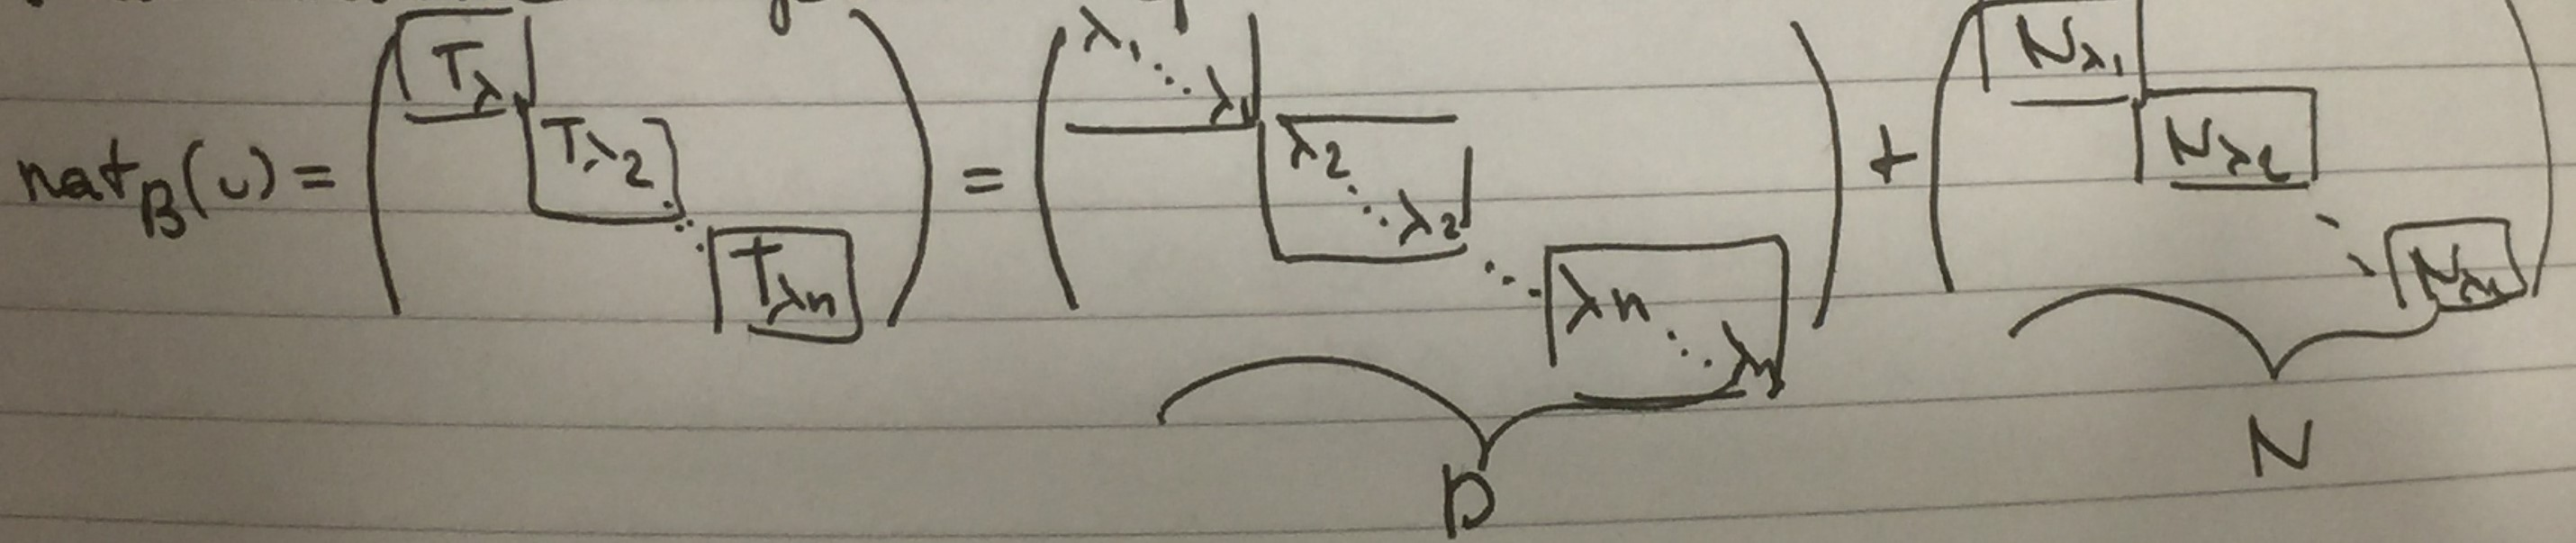
\includegraphics[scale=0.2]{images/001.jpg}\label{maxime}

\end{enumerate}

\subsubsection{Exemple}
Soit u l'endomorphisme de $\R^3$ dont la matrice dans la base canonique est $\begin{pmatrix}
4&0&-1\\1&3&-1\\0&1&2
\end{pmatrix}$.

$P_u(X)=\det(u-X I_n)=\begin{vmatrix}
4-X&0&-1\\1&3-X&-1\\0&1&2-X
\end{vmatrix}=(3-X)^3$.

On a $\begin{pmatrix}x\\y\\z\end{pmatrix}\in E_3\Leftrightarrow \begin{pmatrix}
1&0&-1\\1&0&-1\\0&1&-1
\end{pmatrix}\begin{pmatrix}
x\\y\\z
\end{pmatrix}=\begin{pmatrix}
0\\0\\0
\end{pmatrix}\Leftrightarrow x=y=z$.
Ainsi $E_3=Vect(\begin{pmatrix}
1\\1\\1
\end{pmatrix})$.\\

On a $(A-3I_3)^2=\begin{pmatrix}
1&-1&0\\
1&-1&0\\
1&-1&0
\end{pmatrix}$, $\ker((u-3Id_E)^2)=\{(x,y,z)\tq x=y\}$.

On prend $\epsilon_2=\begin{pmatrix}
1\\1\\0
\end{pmatrix}$,
$(A-3I_3)\epsilon_2=\begin{pmatrix}
1\\1\\1
\end{pmatrix}=\epsilon_1$.
Complétons par $\epsilon_3=\begin{pmatrix}
1\\0\\0
\end{pmatrix}$, $(A-3I_3)\epsilon_3=\epsilon_2$.

$B=(\epsilon_1,\epsilon_2,\epsilon_3)$ est une base de $E$ et $Mat_B(u)=\begin{pmatrix}
3&1&0\\0&3&1\\0&0&3
\end{pmatrix}$, il s'agit d'un bloc de Jordan.

\section{Endomorphismes nilpotents}
\subsection{Définition}
On dit qu'un endomorphisme $u$ de $E$ est nilpotent s'il existe $m\geq 1$ tel que $u^m=0$.\\

L'indice de nilpotence est le plus petit $m\geq 1$ tel que $u^m=0$.

\subsection{Théorème}
$u$ est nilpotent si et seulement si $P_u(x)$ est scindé et $\sigma_\K(u)=\{0\}$.

\subsubsection{Démonstration}
Si $u$ est nilpotent, $\exists n\geq 1$ tel que $u^n=0$.
Soit $\lambda\in \sigma_\K(u)$ et $x$ un vecteur propre associé, $0=u^m(x)=u^{m-1}(u(x))=u^{m-1}(\lambda x)...=\lambda^mx$.\\

Donc $\lambda^m=0$, c'est-à-dire $\lambda=0$. Ceci est possible dans $\C$ car $P_u(x)$ est scindé dans $\C$.
Ainsi $P_u(X))=-x)^n$.\\

La réciproque est évidente.

\subsubsection{Observation}
Nous avons démontré aussi que si $u$ est nilpotent alors son indice de nilpotence est toujours inférieur ou égal à $n=\dim E$.

\subsection{Proposition}
Si $u$ est nilpotent, alors il existe une base $B$ de $E$ dans laquelle la matrice $u$ est triangulaire supérieure stricte.

\subsubsection{Démonstration}
Comme $u$ est nilpotent, on a $\sigma_\K(u)=\{0\}$ et $P_u(x)=(-x)^n$.\\

Ainsi $P_u$ est scindé et $u$ est trigonalisable, il existe une base dans laquelle la matrice de $u$ est triangulaire supérieure (et où sa diagonale n'est composée que de valeurs propres).

\subsubsection{Observation}
La réciproque est vraie aussi.

\subsection{Langage matriciel}
On dit que $A\in M_n(\K)$ est nilpotente s'il existe $m\geq 1$ tel que $A^m=0$.\\

L'indice de nilpotence est le plus petit entier non nul vérifiant $A^m=0$. $A$ est nilpotente si et seulement si $A$ représente dans une base un endomorphisme nilpotent.

\newpage

\subsection{Théorème}
On suppose $\dim E=n\geq 2$.\\
Si $u\in L(E)$ est un endomorphisme nilpotent d'indice $n$, alors il existe une base $B$ de $E$ dans laquelle la matrice de $u$ est nulle sauf les coefficients au dessus de la diagonale qui sont des 1.

\subsubsection{Démonstration}
Comme l'indice de nilpotence est $n$, $\exists x\in E$ tel que $u^{n-1}(x)\neq 0$.\\
Montrons que $B_0=(x,u(x),...,u^{n-1}(x))$ est une base de $E$ en montrant qu'elle est libre.\\

Soit $a_0,...,a_{n-1}\in \K$ tel que $a_0x+a_1u(x)+...+a_{n-1}u^{n-1}(x)=0$.\\

On applique $u^{n-1}$ à cette identité et on trouve que $a_0=0$.\\

De même par composition on obtient que tous les $a_i$ sont nuls.\\

On a $B=(u^{n-1}(x),...,u(x),x)$ et $Mat_B(u)$ est une matrice nulle sauf pour les coefficients au dessus de la diagonale qui valent 1.

\subsubsection{Exemple}
Soit $u$ l'endomorphisme de $R^3$ dont la matrice dans la base canonique est $A=\begin{pmatrix}
1&0&-1\\1&0&-1\\0&1&-1
\end{pmatrix}$.\\

$A$ est nilpotent d'indice 3. Cherchons une base dans laquelle la matrice de $u$ est triangulaire supérieure stricte.\\

$\ker(u^2)=\{(x,y,z)\tq x=y\}$, on prend $x=\begin{pmatrix}
1\\0\\0
\end{pmatrix}$, $u(x)=\begin{pmatrix}
1\\1\\0
\end{pmatrix}$ et $u^2(x)=\begin{pmatrix}
1\\1\\1
\end{pmatrix}$

\section{Réduction de Dunford-Jordan}
\subsection{Théorème}
Soit $u\in L(E)$ dont le polynôme caractéristique est scindé, alors il existe un unique couple $(d,n)$ tel que $d$ est diagonalisable, $n$ est nilpotent, $u=d+n$ et $d\circ n=n\circ d$.\\

En particulier, il existe une base de $E$ dans laquelle la matrice de $u$ s'écrit $T=D+N$ ($D$ est diagonale, $N$ est nilpotente).

\subsubsection{Application}
On veut calculer les puissances successives d'une matrice $A$.\\\\
On commence par calculer $P_A(x)$, puis $E_\lambda$ pour chaque $\lambda\in \sigma_\K(u)$.\\

Si $A$ est diagonalisable, il existe $P$ inversible telle que $A=PDP^{-1}$ et $A^n=PD^nP^{-1}$.\\
Sinon on trigonalise par la méthode de Dunford et $A=P(D+N)P^{-1}$ et $A^m=P^{-1}(D+N)^mP$.\\\\

Les puissances de $(D+N)$ ne contiennent que les puissances de $N$ inférieures à l'indice de nilpotence.
$$(D+N)^m=\sum_{k=0}^m\frac{m!}{k!(m-k)!}D^{m-k}N^k$$

\end{document}
